%%%%%%%%%%%%%%%%%%%%%%%%%%%%%%%%%%%%%
%% Master file SED-ML specification 
%%%%%%%%%%%%%%%%%%%%%%%%%%%%%%%%%%%%%
\listfiles
\documentclass[pdftex,rgb,dvipsnames,svgnames,hyperref,table]{report}
\usepackage{tocvsec2} 

% layout (initialy done for the SBGN project)
\input{sources/styles/latex-style}

% packages and commands
%%%%%%%%%%%%%%%%%%%%%%%%%%%%%%%%%%%%%%%%%%%%%%%%%%%%%%%%%%%%%%%%%%
%%  Commands
%%%%%%%%%%%%%%%%%%%%%%%%%%%%%%%%%%%%%%%%%%%%%%%%%%%%%%%%%%%%%%%%%%

\newcommand{\code}[1]{\texttt{#1}}
\newcommand{\token}[1]{\texttt{#1}}
\newcommand{\concept}[1]{\textcolor{blue}{#1}}
\newcommand{\element}[1]{\texttt{#1}}
\newcommand{\alert}[1]{\textcolor{red}{#1}}
\newcommand{\note}[1]{\paragraph*{} \emph{\scshape{\alert{Please Note}}: #1} \newline}
\newcommand{\mailto}[1]   {\link{mailto:#1}{#1}}
\newcommand{\link}[2]     {\literalFont{\href{#1}{#2}}}
\newcommand{\literalFont}[1]{\textup{\texttt{#1}}}
\newcommand{\version}{2\xspace}
\newcommand{\level}{1\xspace}
\newcommand{\LoneVone}{Level~1 Version~1\xspace}
\newcommand{\LoneVtwo}{Level~1 Version~2\xspace}
\newcommand{\LoneVthree}{Level~1 Version~3\xspace}
\newcommand{\currentLV}{Level~1 Version~3\xspace}
\newcommand{\previousLV}{Level~1 Version~2\xspace}
\newcommand{\biom}{BioModels Database\xspace}
% attribute table layout
\newcommand{\attribute}{attribute\xspace}
\newcommand{\desc}{description\xspace}
\newcommand{\subelements}{sub-elements\xspace}

\newcommand{\SedModel}{\hyperref[class:model]{Model}\xspace}
\newcommand{\SedDataSource}{\hyperref[class:dataSource]{DataSource}\xspace}
\newcommand{\SedDataDescription}{\hyperref[class:dataDescription]{DataDescription}\xspace}
\newcommand{\SedSlice}{\hyperref[class:slice]{Slice}\xspace}

\newcommand{\refpage}[1]{\hyperref[#1]{page \pageref{#1}}} % to hyperref to a particular page in the spec
\newcommand{\tabcap}[1]{  % to create table captions for overview tables for each SED-ML class
Attributes and nested elements for \concept{#1}. \emph{xy$^{o}$} denotes optional elements and attributes.
}

\newcommand{\tabtext}[2]{ % to create the introducing table text for each table reference
\tab{#1}~shows all attributes and sub-elements for the \concept{#2} element as defined by the SED-ML \currentLV XML Schema.
}

\newcommand{\lsttext}[2]{ % to create the introducing listing text for each listing reference
  Listing~\vref{lst:#1} shows the use of the \element{#2} element in a SED-ML file as defined by the SED-ML \currentLV XML Schema.
}

\newcommand{\lsttexta}[2]{ % to create the introducing listing text for each listing reference
  Listing~\vref{lst:#1} shows the use of the \element{#2} attribute in a SED-ML file as defined by the SED-ML \currentLV XML Schema.
}

%
\newcommand{\chap}[1]     {Chapter~\protect\ref{chap:#1}\xspace}
\newcommand{\sect}[1]     {Section~\protect\ref{sec:#1}\xspace}
\newcommand{\fig}[1]      {Figure~\protect\vref{fig:#1}\xspace}
\newcommand{\tab}[1]      {Table~\protect\vref{tab:#1}\xspace}
\newcommand{\lst}[1]      {Listing~\protect\ref{lst:#1}\xspace}
\newcommand{\eg}          {e.\,g.,\xspace}
\newcommand{\ie}          {i.\,e.,\xspace}

\newcommand{\tickYes}{\hspace{1pt}\ding{52}}
\newcommand{\tickNo}{\hspace{1pt}\ding{56}}

%%%%%%%%%%%%%%%%%%%%%%%%%%%%%%%%%%%%%%%%%%%%%%%%%%%%%%%%%%%%%%%%%%
%%  environments
%%%%%%%%%%%%%%%%%%%%%%%%%%%%%%%%%%%%%%%%%%%%%%%%%%%%%%%%%%%%%%%%%%

% standard figure layout
\newcommand{\sedfig}[4][]
	{\begin{figure}[H]\begin{center}{\includegraphics[width=0.9\textwidth,#1]{#2}}\caption{#3}\label{#4}\end{center}\end{figure}}

\newcommand{\sedfigX}[4][]
	{\begin{figure}[H]\begin{center}{\includegraphics[#1]{#2}}\caption{#3}\label{#4}\end{center}\end{figure}}

% standard XML listing layout
\lstnewenvironment{myXmlLst}[2]
	{\lstset{basicstyle=\ttfamily\scriptsize, caption={#1},label={#2}, keywordstyle=\color{blue}\bfseries, stringstyle=\color{blue}, commentstyle=\color{red}, captionpos=b, breaklines=true, xleftmargin=1.5em, xrightmargin=1.5em, numbers=left, numberstyle=\ttfamily\tiny, numbersep=5pt, tabsize=4, showstringspaces=false, language=XML}} %, float=!h
	{}

% listings in appendixes:
\newcommand{\myXmlImport}[3]	{\lstinputlisting[basicstyle=\ttfamily\scriptsize,caption={#1},label={#2},%
	keywordstyle=\color{blue}\bfseries, stringstyle=\color{blue}, commentstyle=\color{red}, captionpos=b, breaklines=true, xleftmargin=1.5em, xrightmargin=1.5em, numbers=left, numberstyle=\ttfamily\tiny, numbersep=5pt, tabsize=4, showstringspaces=false, language=XML, stepnumber=1]{#3}} %float=h!

%%% Local Variables: 
%%% mode: latex
%%% TeX-master: "../sed-ml-L1V3"
%%% End: 




\begin{document}
% =============================================================================
% frontpage
% =============================================================================

\begin{titlepage}

%\vspace*{0.75in}

\begin{center}

  \textbf{\sffamily\bfseries\huge
    Simulation Experiment Description\\ Markup Language (SED-ML) :\\[0.3em]
    Level~1 Version~\changed{4}}

\vspace*{0.5in}

\large
\today\\[0.25in]

%\cornersize{0.3}\ovalbox{\begin{minipage}{4.9in}\color{DarkRed}
%Disclaimer: This is a working draft of the Simulation Experiment 
%Description Markup Language (SED-ML) Level~1 Version~3 specification.  
%It is not a normative document.
%\end{minipage}}

\vspace{0.5in}

\textbf{\sffamily Editors}\\[7pt]
\begin{tabular}{l>{\hspace*{15pt}}r}
Frank T Bergmann & \emph{Caltech, USA}\\
Jonathan Cooper & \emph{University of Oxford, UK}\\
Matthias K\"{o}nig & \emph{Humboldt University Berlin, Germany}\\
Ion Moraru & \emph{University of Connecticut, USA}\\
David Nickerson & \emph{Auckland Bioengineering Institute, New Zealand}\\
Nicolas Le Nov{\`e}re & \emph{Babraham Institute Cambridge, UK}\\
Brett G Olivier & \emph{University Amsterdam, Netherlands}\\
Sven Sahle & \emph{Heidelberg University, Germany}\\
Lucian Smith & \emph{University of Washington, USA}\\
Dagmar Waltemath & \emph{University of Rostock, Germany}
\end{tabular}
 
\vspace{1.2in}

\normalsize
\begin{minipage}{5in}
\begin{center}
  The latest release of the \currentLV specification is available at
  \url{http://identifiers.org/combine.specifications/sed-ml.level-1.version-4}
  \paragraph*{}
  To discuss SED-ML and the SED-ML specification write to the mailing list \mailto{sed-ml-discuss@googlegroups.com}.

  \paragraph*{}
  To contact the SED-ML editors write to \mailto{sed-ml-editors@googlegroups.com}.
\end{center}
\end{minipage}
\vfill


\centerline{\includegraphics[width=2in]{images/logoSedml.png}}

\end{center}

\end{titlepage}

% The title page is considered unnumbered and the next page after this
% starts with the page number 1 (actually, i), but the duplication of page
% number 1 confuses hyperref and leads to the following latex warning:
%
%   "pdfTeX warning (ext4): destination with the same identifier
%   (name{page.1}) has been already used, duplicate ignored"
%
% The following change makes the title page have page number 1 and the next
% page after that it becomes page ii.  This is unorthodox, but seems not
% completely unreasonable, and it avoids the confusing warning above.

\setcounter{page}{2}



%%% Local Variables: 
%%% mode: latex
%%% TeX-master: "../sed-ml-L1V3"
%%% End: 

\tableofcontents
\newpage
% ~~~~~~~~~~~~~~~~~~~~~~~~~~~~~~~~~~~~~~~~
%% INTRODUCTION
% ~~~~~~~~~~~~~~~~~~~~~~~~~~~~~~~~~~~~~~~~
% ~~~~~~~~~~~~~~~~~~~~~~~~~~~~~~~~~~~~~~~~
%% INTRODUCTION
% ~~~~~~~~~~~~~~~~~~~~~~~~~~~~~~~~~~~~~~~~
\chapter{Introduction}
The Simulation Experiment Description Markup Language (SED-ML) is an XML-based format for the description of simulation experiments.

The number of computational models of biological systems is growing at an ever increasing pace. 
At the same time, their size and complexity are also increasing. It is now generally accepted that one must be able to exchange the mathematical structure of such models, for instance to build on existing studies by reusing models or for the reproduction of model results. The efforts to standardise the representation of computational models in various areas of biology, such as the Systems Biology Markup Language (SBML) \citep{Hucka:2003}, CellML \citep{cuellar:2003} or NeuroML \citep{Goddard:2001}, resulted in an increase of the exchange and re-use of models. 

However, the description of the structure of models is not sufficient for the reproduction of simulation results. One also needs to describe the procedures the models are subjected to, i.e. the minimal set of information that should be provided to allow the reproduction of simulation experiments among users and software tools as described by the Minimum Information About a Simulation Experiment (MIASE \citep{Waltemath:2011}). The increasing use of computational simulation experiments to inform modern biological research creates new challenges to reproduce, annotate, archive, and share such experiments. 

SED-ML describes in a computer-readable exchange format the information to enable the reproduction of simulation experiments. SED-ML is a software-independent format encoded in the Extensible Markup Language (XML) \citep{Bray:2006} not specific to particular simulation tools and independent of the underlying model implementation.

SED-ML is developed as a community project and defined via a detailed technical specification and a corresponding XML Schema. 

This document describes \currentLV of SED-ML which is the successor of \previousLV and \LoneVone (described in \citep{WAB+11}).

% ~~~~~~~~~~~~~~~~~~~~~~~~~~~~~~~~~~~~~~~~
%% OVERVIEW
% ~~~~~~~~~~~~~~~~~~~~~~~~~~~~~~~~~~~~~~~~
\section{SED-ML overview}
SED-ML specifies for a given simulation experiment

\begin{itemize}
\item what datasets to use (\hyperref[class:dataDescription]{DataDescription})
\item which models to use in an simulation experiment (\hyperref[class:model]{Model})
\item which modifications to apply to models before simulation (\hyperref[class:change]{Change}) 
\item which simulation procedures to run on each model (\hyperref[class:simulation]{Simulation} and \hyperref[class:task]{Task})
\item what analysis results to plot or report and how to post-process (\hyperref[class:dataGenerator]{DataGenerator})
\item and how these results should be presented (\hyperref[class:output]{Output})
\end{itemize}

A \hyperref[class:sed-ml]{SED-ML document} containts the following main objects to describe this information: \hyperref[class:dataDescription]{DataDescription}, \hyperref[class:model]{Model}, \hyperref[class:change]{Change}, \hyperref[class:simulation]{Simulation}, \hyperref[class:task]{Task}, \hyperref[class:dataGenerator]{DataGenerator}, and \hyperref[class:output]{Output}.

\paragraph*{\hyperref[class:dataDescription]{DataDescription}}
The \hyperref[class:dataDescription]{DataDescription} allows to specify data sets used in a simulation experiment. Such data can be used for instance for parametrization of model simulations or to plot data with simulation results.

\paragraph*{\hyperref[class:model]{Model}}
The \hyperref[class:model]{Model} is used to reference the models used in the simulation experiment. SED-ML itself is independent of the model encoding underlying the models.

The SED-ML \hyperref[class:change]{Change} allows the application of changes to the referenced models (pre-processing), including changes on the XML attributes, e.g. changing the value of an observable, computing the change of a value using mathematics, or general changes on any XML element of the model representation that is addressable by \hyperref[sec:xpath]{XPath} expressions, e.g. substituting a piece of XML by an updated one.

\paragraph*{\hyperref[class:simulation]{Simulation}}
The \hyperref[class:simulation]{Simulation} defines the simulation settings and the steps taken during simulation. These include the particular type of simulation and the algorithm used for the execution of the simulation.

\paragraph*{\hyperref[class:task]{Task}}
SED-ML uses the concept of \hyperref[class:task]{Task} to combine a defined \hyperref[class:model]{Model} and \hyperref[class:simulation]{Simulation}.

\paragraph*{\hyperref[class:dataGenerator]{DataGenerator}}
The \hyperref[class:dataGenerator]{DataGenerator} allows to encode post-processing of simulation results before output, e.g. one might want to normalise a plot before output, or apply post-processing like mean-value calculation. In the definition of a \hyperref[class:dataGenerator]{DataGenerator}, any addressable variable or parameter of any defined model may be referenced, and new entities might be specified using \hyperref[sec:mathML]{MathML}.

\paragraph*{\hyperref[class:output]{Output}}
The \hyperref[class:output]{Output} defines the output of the simulation, which can be either a two dimensional plot \hyperref[class:plot2D]{Plot2D}, a three dimensional plot \hyperref[class:plot3D]{Plot3D}, or data table \hyperref[class:report]{Report}. The \hyperref[class:output]{Output} is based on the \hyperref[class:dataGenerator]{DataGenerators}.

This section provided a high level overview over the content of a SED-ML file. For the detailed technical specification see Chapter~\ref{chp:specification}. 

% ~~~~~~~~~~~~~~~~~~~~~~~~~~~~~~~~~~~~~~~~
%% EXAMPLE SIMULATION
% ~~~~~~~~~~~~~~~~~~~~~~~~~~~~~~~~~~~~~~~~
\section{Example simulation experiment}
\label{motivation:example}
In this section an introductory example is given how simulation experiments can be described with SED-ML. The example experiment uses the repressilator \citep{Elowitz:2000} a famous model capable of displaying rich and variable behaviors. The SED-ML for the presented simulation experiment is listed in Appendix~\ref{example:repressilator}.

The repressilator is a synthetic oscillating network of transcription regulators in Escherichia coli. The network is composed of the three repressor genes Lactose Operon Repressor (lacI), Tetracycline Repressor (tetR) and Repressor CI (cI), which code for proteins binding to the promoter of the other, blocking their transcription. The three inhibitions together in tandem, form a cyclic negative-feedback loop. To describe the interactions of the molecular species involved in the network, the authors built a simple mathematical model of coupled first-order differential equations. All six molecular species included in the network (three mRNAs, three repressor proteins) participated in creation (transcription/translation) and degradation processes. The model was used to determine the influence of the various parameters on the dynamic behavior of the system. In particular, parameter values were sought which induce stable oscillations in the concentrations of the system components. Oscillations in the levels of the three repressor proteins can be obtained by numerical integration. 

\hl{TODO MK: add sample experiment to examples in appendix}
\hl{TODO MK: create simulation results with tellurium and SED-ML webtools to show reproducibility}

%% ~~ TIMECOURSE ~~
\subsection{Time-course simulation}
\label{sec:timecourse}
The first simulation experiment we run with the model reproduces the oscillation behavior of the model shown in Figure~1c of the reference publication \citep{Elowitz:2000}. This simulation experiment can be described as:

\begin{enumerate}
 	\item{Import the model identified by the Unified Resource Identifier (URI) \citep{Berners-Lee:2005}\\ 	\url{urn:miriam:biomodels.db:BIOMD0000000012}.}
 	\item {Select a deterministic simulation method.}
 	\item{Run a uniform time course simulation for 1000~min with an output interval of 1~min.}
 	\item{Plot the amount of \code{lacI}, \code{tetR} and \code{cI} against time in a 2D Plot.}
 \end{enumerate}

Following those steps and performing the simulation in the simulation tools supporting SED-ML results in the output depicted in \fig{rep_tc}. \hl{TODO: legend and xaxis label missing, rerun with tellurium and SED-ML webtools.}

\begin{figure}[ht]
	\centering
	\includegraphics[width=0.6\textwidth]{examples/repressilator/rep_tc}
	\caption{Time-course simulation of the repressilator model, imported from BioModels Database and simulated in COPASI. The number of repressor proteins lacI, tetR and cI is depicted.}
	\label{fig:rep_tc}
\end{figure}


%% ~~ PRE-PROCESSING ~~
\subsection{Applying pre-processing}
\label{sec:preprocessing}
Before simulation model parameters can be adjusted. When changing the parameter values \emph{protein copies per promoter} \code{tps$\_$repr} and \emph{leakiness in protein copies per promoter} \code{tps$\_$active} like depicted below, the system's behavior switches from sustained oscillations to damped oscillations towards an asymptotic steady-state. The model changes leading to that behavior are described as: 

\begin{enumerate}
	\item{Import the model as above.}
	\item{Change the value of the parameter \code{tps$\_$repr} from “0.0005” to “1.3e-05”.}
	\item{Change the value of the parameter \code{tps$\_$active} from “0.5 “ to “0.013“.}
	\item{Select a deterministic method.}
	\item{Run a uniform time course for the duration of 1000~min with an output interval of 1~min.}
	\item Plot the amount of lacI, tetR and cI against time in a 2D Plot.
\end{enumerate}

\fig{rep_pre} shows the result of the simulation.

\begin{figure}[ht]
	\centering
	\includegraphics[width=0.7\textwidth]{examples/repressilator/rep_pre.png}
	\caption{Time-course simulation of the repressilator model, imported from BioModels Database and simulated after modification of the initial parameter values of the \emph{protein copies per promoter} and the \emph{leakiness in protein copies per promoter}. The number of repressor proteins lacI, tetR and cI are depicted.}
	\label{fig:rep_pre}
\end{figure}

%% ~~ POST-PROCESSING ~~
\subsection{Applying post-processing}
\label{sec:postprocessing}
The raw numerical output of the simulation steps may be subjected to data post-processing before plotting or reporting. In order to describe the production of a normalized plot of the time-course in the first example (section \ref{sec:timecourse}), depicting the influence of one variable on another (in phase-planes), one performes the additional steps:

(Please note that the description steps 1 - 4 remain as given in section \ref{sec:timecourse} above.)
\begin{enumerate}
	\item[5.]{Collect lacI(t) , tetR(t) and cI(t).}
	\item[6.]{Compute the highest value for each of the repressor proteins, max(lacI(t)), max(tetR(t)), max(cI(t)).}
	\item[7.]{Normalize the data for each of the repressor proteins by dividing each time point by the maximum value, i.\,e.\ lacI(t)/max(lacI(t) ), tetR(t)/max(tetR(t)) , and cI(t)/max(cI(t)).}
	\item[8.]{Plot the normalized \code{lacI} protein as a function of the normalized \code{cI}, the normalized \code{cI}  as a function of the normalized \code{tetR} protein, and the normalized \code{tetR} protein against the normalized \code{lacI} protein in a 2D plot.}
\end{enumerate}

\fig{rep_post} illustrates the result of the simulation after post-processing of the output data. 
	\begin{figure}[ht]
	\centering
	\includegraphics[width=0.7\textwidth]{examples/repressilator/rep_post.png}
	\caption{Time-course simulation of the repressilator model imported from BioModels Database and simulated with COPASI. Depicted is the normalized temporal evolution of lacI, tetR and cI in phase-plane.}
	\label{fig:rep_post}
\end{figure}


% ~~~~~~~~~~~~~~~~~~~~~~~~~~~~~~~~~~~~~~~~
%% TECHNICAL SPECIFICATION
% ~~~~~~~~~~~~~~~~~~~~~~~~~~~~~~~~~~~~~~~~
\chapter{SED-ML technical specification}
\label{chp:specification}
This document represents the technical specification of SED-ML \currentLV. The corresponding UML class diagram is shown in \fig{sedML}. Example simulation experiments in SED-ML are provided in Appendix~\ref{app:examples}. The XML Schema is provided in Appendix~\ref{app:schema}. However, not all concepts of SED-ML can be captured using XML Schema alone. In such cases this specification is the normative document. 

\sedfig[width=\textwidth]{images/uml/all}{The SED-ML \currentLV UML class diagram}{fig:sedML}

%% ~~~ NOTATION CONVENTIONS ~~~
%% THIS PROVIDES NO INFORMATION AT ALL, ON THE CONTRARY IT CONFUSES READER 
%% \section{Conventions used in this document}
\label{sec:conventions}


%% UML
\subsection{UML Classes}
\label{sec:umlconventions}
A SED-ML UML class (\fig{umlClass}) consists of a class name (\code{ClassName}) and a number of attributes (\code{attribute}) each of a specific data type (\code{type}). The SED-ML UML specification does not make use of UML \code{operations}.
\begin{figure}[h]
\centering
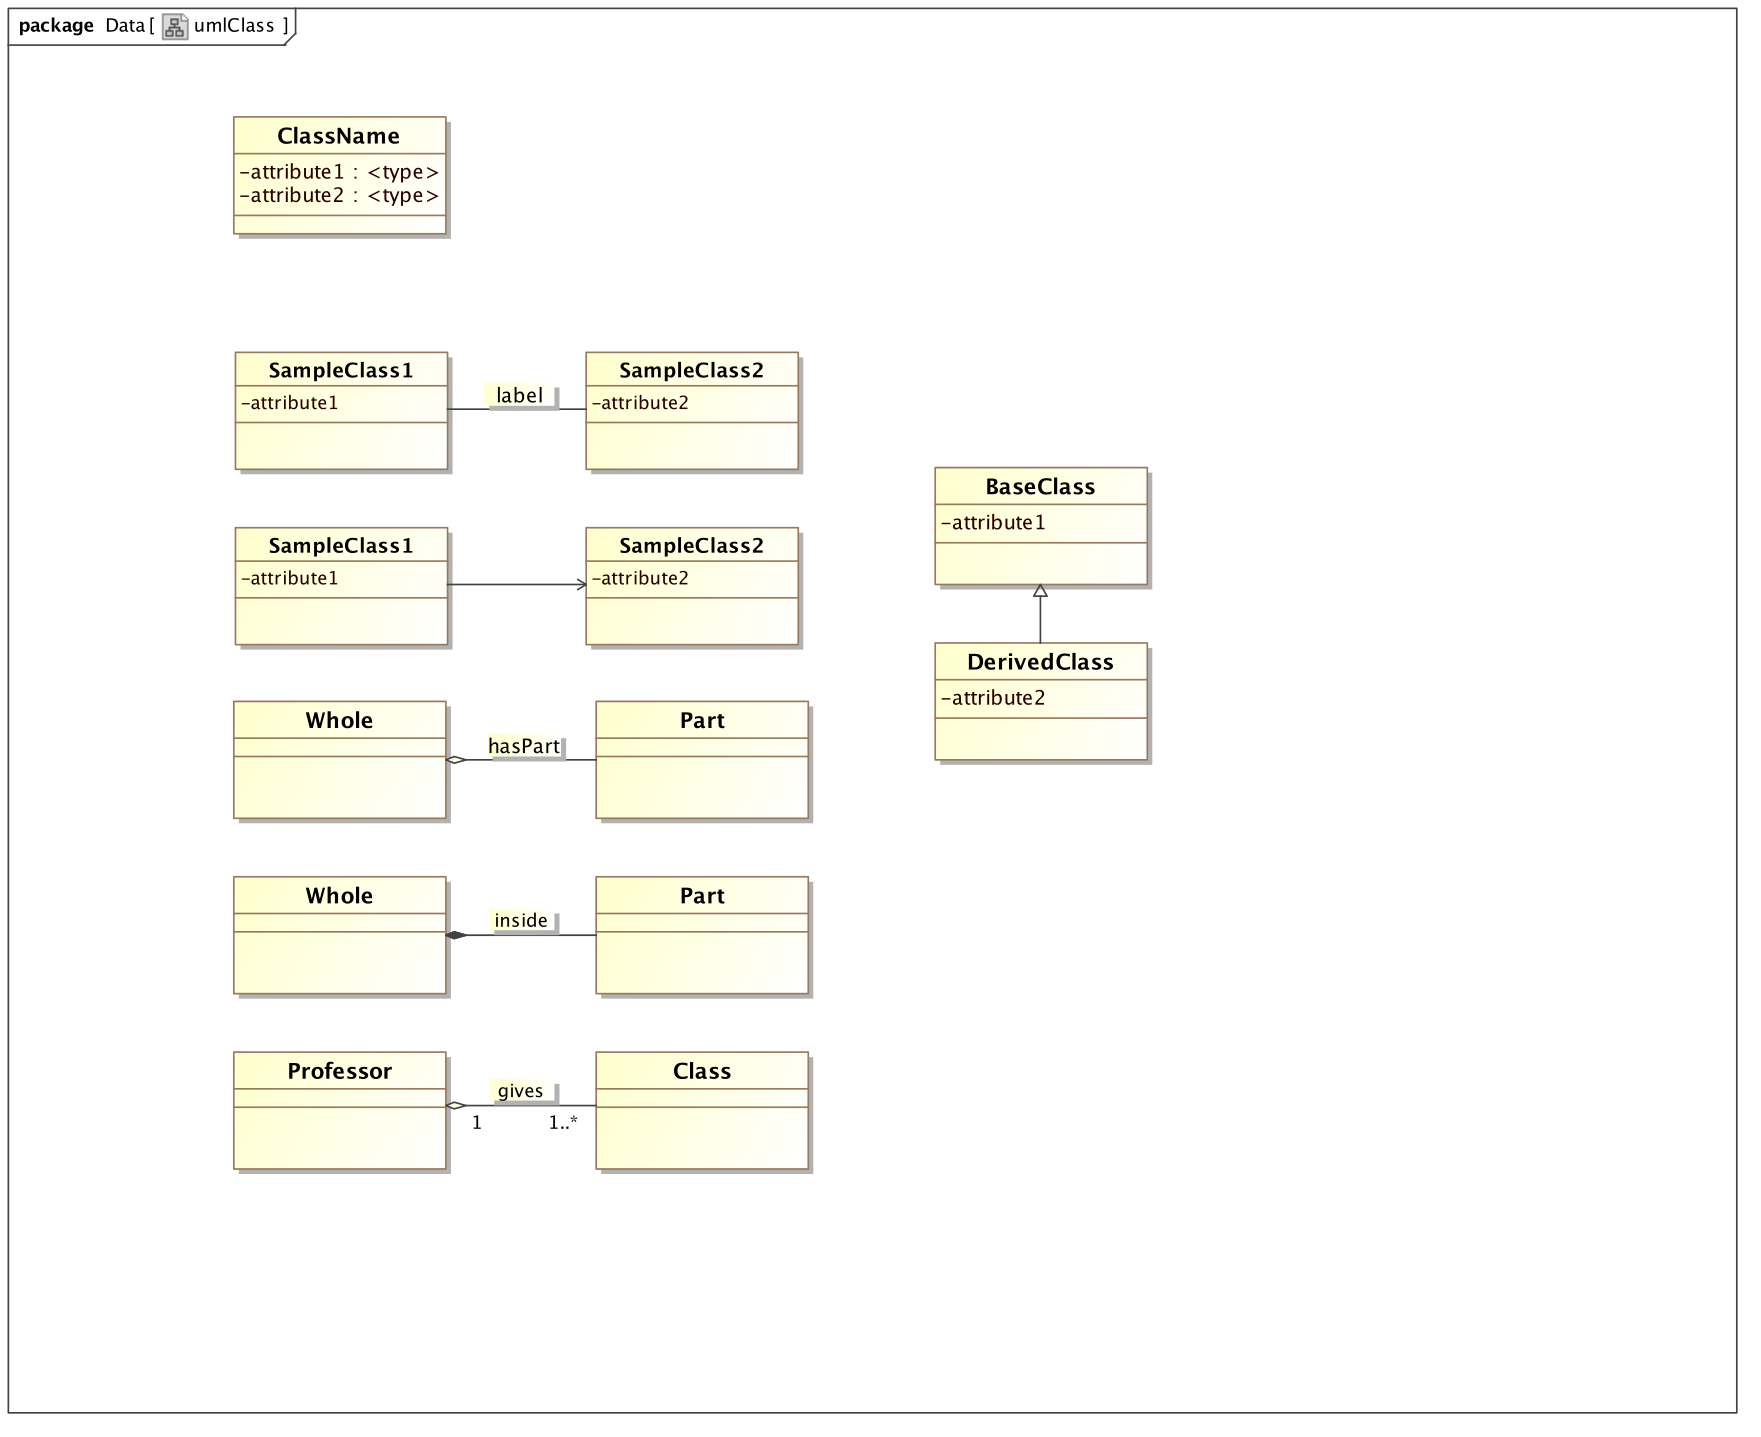
\includegraphics[width=0.2\textwidth]{images/uml/umlClass.png}
\caption{SED-ML UML Class with class names and attributes}
\label{fig:umlClass}
\end{figure}

SED-ML class names always begin with upper case letters. If they are composed of different words, the camel case style is used, as in e.\,g.\ \code{DataGenerator}.

\subsection{UML Relationships}
%% RELATIONS
\subsubsection{UML Relation Types}
\begin{figure}[h]
\centering
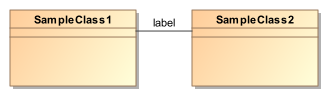
\includegraphics[width=0.5\textwidth]{images/uml/classRelation.png}
\caption{UML Class connectors}
\label{fig:umlConnectors}
\end{figure}

Links between classes specify the connection of objects with each other (\fig{umlConnectors}). The different relation types used in the SED-ML specification include aggregation, composite aggregation, and generalisation. The label on the line is called symbol (\code{label}) and describes the relation of the objects of both classes. 

%% Association
The \concept{association} (\fig{umlAssociation}) indicates the existence of a connection between the objects of the participating classes. Often associations are directed to show how the label should be read (in which direction). Associations can be uni-directional (one arrowhead), or bidirectional (zero or two arrowheads). 
\begin{figure}[h]
\centering
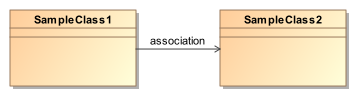
\includegraphics[width=0.5\textwidth]{images/uml/umlAssociation.png}
\caption{UML Association}
\label{fig:umlAssociation}
\end{figure}

 
%% Aggregation
The \concept{aggregation} (\fig{umlAggregation}, top) indicates that the objects of the participating classes are connected in a way that one class (\code{Whole}) consists of several parts (\code{Part}). In an aggregation, the parts may be independent of the whole. For example, a car (\code{Whole})  has several parts called wheel (\code{Part}); however, the wheels can exist independently of the car while the car requires the wheels in order to function.
\begin{figure}[h]
\centering
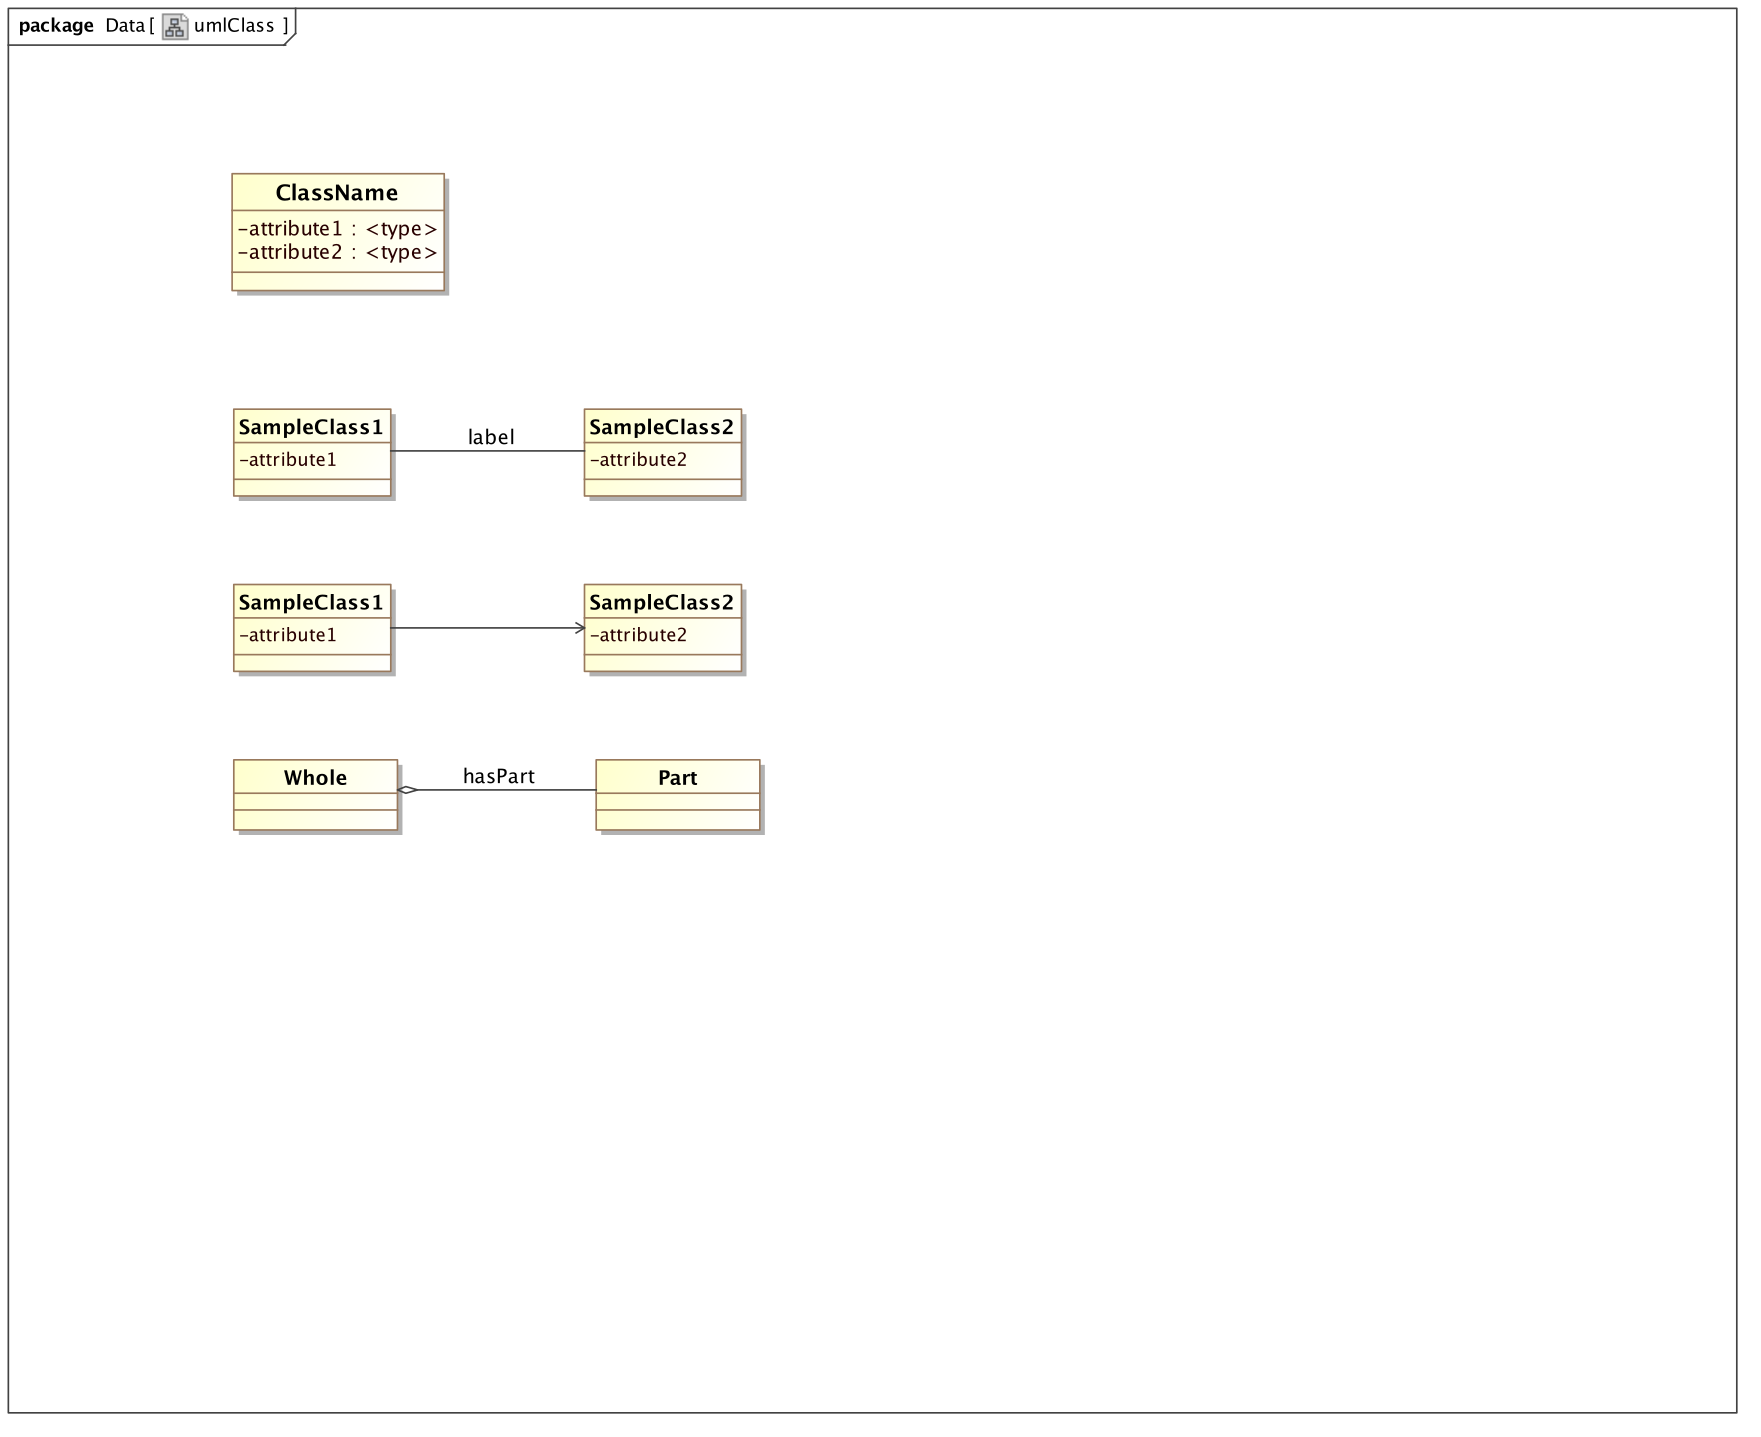
\includegraphics[width=0.5\textwidth]{images/uml/umlAggregation.png}
\caption{UML Aggregation}
\label{fig:umlAggregation}
\end{figure}

%% Composite Aggregation
The \concept{composite aggregation} (\fig{umlAggregation}, bottom) indicates that the objects of the participating classes are connected in a way that one class (\code{Whole}) consists of several parts (\code{Part}). In contrast to the aggregation, the subelements (\code{Part}) are dependent on the parent class (\code{Whole}). An example is that a university (\code{Whole}) consists of a number of departments (\code{Part}) which have a so-called ``lifetime responsibility'' with the university, e.\,g.\ if the university vanishes,  the departments will vanish with it \citep{Bel03}.

%% Inheritance
The \concept{generalisation} (\fig{umlGeneralisation}) allows to extend classes (\code{BaseClass}) by additional properties. The derived class (\code{DerivedClass}) inherites all properties of the base class and defines additional ones. In the given example, an instance of \code{DerivedClass} has two attributes \code{attribute1} and \code{attribute2}.
%
\begin{figure}[h]
\centering
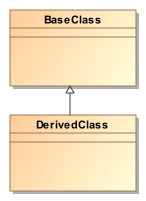
\includegraphics[width=0.2\textwidth]{images/uml/umlGeneralisation.png}
\caption{UML Generalisation}
\label{fig:umlGeneralisation}
\end{figure}
%
%% CARDINALITIES
\subsubsection{UML multiplicity}
UML multiplicity defines the number of objects in one class that can be related to one object in the other class (also known as \concept{cardinality}). Possible types of multiplicity include values (1), ranges (1$..$4), intervals (1,3,9), or combinations of ranges and intervals. The standard notation for ``many'' is the asterix (*). 

Multiplicity can be defined for both sides of a relationship between classes. The default relationship is ``many to many''. 
The example in \fig{umlMulti} expresses that a class is given by a professor, and a professor might give one to many classes.
\begin{figure}[h]
\centering
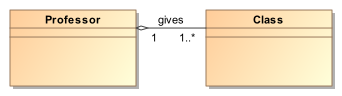
\includegraphics[width=0.4\textwidth]{images/uml/umlMultiplicity.png}
\caption{UML Multiplicity in an Aggregation}
\label{fig:umlMulti}
\end{figure}

%% XML SCHEMA
\subsection{XML Schema language elements}
The main building blocks of an XML Schema specification are:
\begin{itemize}
\item {simple and complex types}
\item {element specifications}
\item {attribute specifications}
\end{itemize}
XML Schema \concept{definitions} create new types, \concept{declarations} define new elements and attributes.
The definition of new (simple and complex) types can be based on a number of already existing, prefedined types (string, boolean, float). Simple types are restrictions or extensions of predefined types. Complex types describe how attribues can be assigned to elements and how elements can contain further elements. The current SED-ML XML Schema only makes use of \emph{complex type definitions}.
An example for a complex type definition is given in \lst{complexType}:
%
\begin{myXmlLst}{Complex Type definition of the SED-ML \code{computeChange} element}{lst:complexType}
<xs:element name="computeChange">
		<xs:complexType>
			<xs:complexContent>
				<xs:extension base="SEDBase">
					<xs:sequence>
						<xs:element ref="listOfVariables" minOccurs="0" />
						<xs:element ref="listOfParameters" minOccurs="0" />
						<xs:element ref="math" />
					</xs:sequence>
					<xs:attribute name="target" use="required" type="xs:token" />
				</xs:extension>
			</xs:complexContent>
		</xs:complexType>
	</xs:element>
\end{myXmlLst}
%
It shows the declaration of an element called \code{computeChange} that is used in SED-ML to change mathematical expressions. The element is defined using an \emph{unnamed} complex type which is build of further elements called \code{listOfVariables}, \code{listOfParameters}, and \code{math}. 
Additionally, the element \code{computeChange} has an attribute \code{target} declared. Please note that the definition of the elements inside the complex type are only referred to and will be found elsewhere in the schema.

The nesting of elements in the schema can be expressed using the \code{xs:sequence} (a sequence of elements), \code{xs:choice} (an alternative of elements to choose from), or \code{xs:all} (a set of elements that can occur in any order) concepts. The current SED-ML XML Schema only uses the \emph{sequence} of elements. 

\subsubsection{Multiplicities}
The standard multiplicity for each defined \code{element} is 1. Explicit multiplicity is to be defined using the \code{minOccurs} and \code{maxOccurs} attributes inside the complex type definition, as shown in \lst{multiplicity}.

\begin{myXmlLst}{Multiplicity for complex types in XML Schema}{lst:multiplicity}
<xs:element name="dataGenerator">
		<xs:complexType>
			<xs:complexContent>
				<xs:extension base="SEDBase">
					<xs:sequence>
						<xs:element ref="listOfVariables" minOccurs="0" />
						<xs:element ref="listOfParameters" minOccurs="0" />
						<xs:element ref="math" />
					</xs:sequence>
					<xs:attributeGroup ref="idGroup" />
				</xs:extension>
			</xs:complexContent>
		</xs:complexType>
	</xs:element>
\end{myXmlLst}
%
In this example, the \code{dataGenerator} type is build of a sequence of three elements: The \code{listOfVariables} element is not necessary for the definition of a valid \code{dataGenerator} XML structure (it may occur 0 times or once). The same is true for the \code{listOfParameters} element (it may as well occur 0 times or once). The \code{math} element, however, uses the implicit standard multiplicity -- it must occur exactly 1 time in the \code{dataGenerator} specification.

\subsection{Type extensions}
XML Schema offers mechanisms to restrict and extend previously defined complex types. Extensions add element or attribute declarations to existing types, while restrictions restrict the types by adding further characteristics and requirements (facets) to a type. An example for a type extension is given in \lst{xmlExtension}.
%
\begin{myXmlLst}{Definition of the sedML type through extension of SEDBase in SED-ML}{lst:xmlExtension}
	<xs:element name="sedML">
		<xs:complexType>
			<xs:complexContent>
				<xs:extension base="SEDBase">
					<xs:sequence>
						<xs:element ref="listOfSimulations" minOccurs="0" />
						<xs:element ref="listOfModels" minOccurs="0" />
						<xs:element ref="listOfTasks" minOccurs="0" />
						<xs:element ref="listOfDataGenerators" minOccurs="0" />
						<xs:element ref="listOfOutputs" minOccurs="0" />
					</xs:sequence>
					<xs:attribute name="level" type="xs:decimal" use="required"
						fixed="1" />
					<xs:attribute name="version" type="xs:decimal" use="required"
						fixed="1" />
				</xs:extension>
			</xs:complexContent>
		</xs:complexType>
	</xs:element>
\end{myXmlLst}
%
%% Q: How about renaming sedML to sed-ml for the next version?
The \code{sedML} element is an extension of the previously defined \code{SEDBase} type. It extends \code{SEDBase} by a sequence of five additional elements (\code{listOfSimulations}, \code{listOfModels}, \code{listOfTasks}, \code{listOfDataGenerators}, and \code{listOfOutputs}) and a new attribute \code{version}.

%% MAPPINGS
% \subsection{Mappings}

% \subsubsection{Mapping the Workflow Structure to a UML Class Diagram Structure}
% The main structure of the above shown workflow can be easily recognised in main class structure of the UML class diagram as shown in Figure \ref{fig:sedml}. Other processes of the workflow have been mapped to according class attributes and/or additional classes in the UML class diagram structure.

% \subsubsection{Conversion of UML into XML Schema}
% Also, the conversion of the UML class diagram representation into the XML Schema model is very intuitive and follows a small set of rules: UML Classes from the diagram are mapped to XML \alert{tbc}
% Page 6 of the SBML spec


%%% Local Variables: 
%%% mode: latex
%%% TeX-master: "../sed-ml-L1V2"
%%% End: 


%% ~~~ CONCEPTS ~~~
\section{Concepts used in SED-ML}

  %% MATHML SUBSET USED
  % on the MathML subset used in SED-ML
\label{sec:mathML}
\subsection{The MathML Subset used in SED-ML}
The SED-ML specification allows for the pre-processing of computational models, 
as well as post processing of the simulation results. The corresponding 
mathematical expressions are encoded using MathML 2.0. MathML is an 
international standard for encoding mathematical expressions using XML and is 
used as representation of mathematical expressions in SBML and CellML, two of 
the languages supported by SED-ML. A problem arises, because the individual 
supported model exchange languages allow different subsets of MathML. Thus, 
when for example a ChangeXML element replaces a mathematical expression of  an 
SBML reaction, only the MathML subset allowed by SBML should be used here. 

In order to make the SED-ML format easier to adopt, at the beginning we 
restrict the MathML subset to the following operations: 

\begin{itemize}\setlength{\parskip}{-0.1ex}

\item \emph{token}: \token{cn}, \token{ci}, \token{csymbol},
  \token{sep}
  
\item \emph{general}: \token{apply}, \token{piecewise},
  \token{piece}, \token{otherwise}, \token{lambda} 

\item \emph{relational operators}: \token{eq}, \token{neq},
  \token{gt}, \token{lt}, \token{geq}, \token{leq}

\item \emph{arithmetic operators}: \token{plus}, \token{minus},
  \token{times}, \token{divide}, \token{power}, \token{root},
  \token{abs}, \token{exp}, \token{ln}, \token{log},
  \token{floor}, \token{ceiling}, \token{factorial}

\item \emph{logical operators}: \token{and}, \token{or},
  \token{xor}, \token{not}

\item \emph{qualifiers}: \token{degree}, \token{bvar},
  \token{logbase}

\item \emph{trigonometric operators}: \token{sin}, \token{cos},
  \token{tan}, \token{sec}, \token{csc}, \token{cot},
  \token{sinh}, \token{cosh}, \token{tanh}, \token{sech},
  \token{csch}, \token{coth}, \token{arcsin}, \token{arccos},
  \token{arctan}, \token{arcsec}, \token{arccsc}, \token{arccot},
  \token{arcsinh}, \token{arccosh}, \token{arctanh},
  \token{arcsech}, \token{arccsch}, \token{arccoth}

\item \emph{constants}: \token{true}, \token{false},
  \token{notanumber}, \token{pi}, \token{infinity},
  \token{exponentiale}

\item \emph{MathML annotations}: \token{semantics},
  \token{annotation}, \token{annotation-xml}

\end{itemize}

It should be noted, that all the operations listed above, only operate on 
singular values. However, as one of SED-ML's aim is to provide post processing 
on the results of simulation experiments, we need to enhance this basic set of 
operations by some aggregate functions. 

\subsubsection{Enabling post processing of simulation experiments}

The first step for enabling for post processing, is to define the symbols that 
represent vector values. To simplify things for SED-ML L1V1 the only symbols to 
be used are the identifiers of variables defined in the listOfVariables of 
DataGenerators. These variables represent the data collected from the 
simulation experiment with the associated task. 

To enable post processing the following aggregate functions are available for 
use with DataGenerator variables: 

\begin{itemize}\setlength{\parskip}{-0.1ex}

\item \emph{min}: Where the minimum of a variable represents the smallest value 
the simulation experiment yielded. Example: 

\begin{verbatim} <min> <ci> variableId </ci></min> \end{verbatim}.

\item \emph{max}: Where the maximum of a variables represents the largest value 
the simulation experiment yielded. Example: 

\begin{verbatim} <max> <ci> variableId </ci></max> \end{verbatim}.

\item \emph{sum}: All values of the variable returned by the simulation 
experiment are added up. Example: 

\begin{verbatim} <sum> <ci> variableId </ci></sum> \end{verbatim}.

\item \emph{product}: All values of the variable returned by the simulation 
experiment are multiplied. Example: 

\begin{verbatim} <product> <ci> variableId </ci></product> \end{verbatim}.

\end{itemize}

These represent the only exceptions. At this point SED-ML does not define a 
complete algebra of vector values. For more information see the description of 
DataGenerators.

%%% Local Variables: 
%%% mode: latex
%%% TeX-master: "../sed-ml-L1V1"
%%% End: 


  %% THE SUGGESTED URI SCHEME
  % The proposed URI scheme to use
  \subsection{URI Scheme}  
\label{sec:uriScheme}

URIs are needed at different points in SED-ML \LoneVtwo: 
Firstly, they are the preferred mechanism to refer to model encodings. 
Secondly, they are used to specify the language of the referenced model.
Thirdly, they enable addressing implicit model variables.
Finally, annotations of SED-ML elements should be provided with a standardised annotation scheme.

The use of a standardised URI Scheme ensures long-time availability  of particular information that can unambiguously be identified. 

\subsubsection{Model references}
\label{sec:modelURI}
The preferred way for referencing a model from a SED-ML file is adopted from the \concept{MIRIAM URI Scheme}.
MIRIAM enables identification of a data resource (in this case a model resource) by a predefined URN. A data entry inside that resource is identified by an ID. 
That way each single  model  in a particular model repository can be unambiguously referenced. To become part of MIRIAM resources, a model repository must ensure permanent and consistent model references, that is stable IDs.

One model repository that is part of MIRIAM resources is the \concept{BioModels Database} \citep{LDR+10}. Its data resource name in MIRIAM is \code{urn:miriam:biomodels.db}. To refer to a particular model, a standardised identifier scheme is defined in \concept{MIRIAM Resources}\footnote{\url{http://www.ebi.ac.uk/miriam/}}. The ID entry maps to a particular model in the model repository. That model is never deleted. 
A sample BioModels Database ID is \code{BIOMD0000000048}. Together with the data resource name it becomes unambiguously identifiable by the URN \code{urn:miriam:biomodels.db:BIOMD0000000048} (in this case referring to the 1999 Kholodenko model on EGFR signaling). 
%

SED-ML recommends to follow the above scheme for model references, if possible. 
SED-ML does not specify how to resolve the URNs. However, MIRIAM Resources offers web services to do so\footnote{\url{http://www.ebi.ac.uk/miriam/}}. For the above example of the \code{urn:miriam:biomodels.db:BIOMD0000000048} model, the resolved URL may look like: 
\begin{itemize}
 \item{\code{http://biomodels.caltech.edu/BIOMD0000000048} or}
 \item{\code{http://www.ebi.ac.uk/biomodels-main/BIOMD0000000048}}
\end{itemize}
depending on the physical location of the resource chosen to resolve the URN.

An alternative means to obtain a model may be to provide a single resource containing necessary models and a SED-ML file. Although a specification of such a resource is beyond the scope of this document,  one proposal  --  SED-ML archive format -- is  described   in Appendix~\ref{app:archive}.
Further information on the \hyperref[sec:source]{source} attribute referencing the model location is provided in Section~\ref{sec:source}.

\subsubsection{Language references}
\label{sec:languageURI}
To specify the language a model is encoded in, a set of pre-defined SED-ML URNs can be used. 
The structure of SED-ML language URNs is \element{urn:sedml:language:}\emph{name.version}. 
SED-ML allows to specify a model representation format very generally as being \code{XML}, if no standardised representation format has been used to encode the model. On the other hand, one can be as specific as defining
a model being in a particular version of a language, as ``SBML Level 2, Version 2, Revision 1''.

The list of URNs is available from \url{http://sed-ml.org/}. 
Further information on the \hyperref[sec:language]{language} attribute is provided in Section~\ref{sec:language}.

\subsubsection{Implicit variables}
\label{sec:implicitVariable}

Some variables used in an experiment are not explicitly defined in the model, but may be implicitly contained in it. 
For example, to plot a variable's behaviour over time, that variable is defined in an SBML model, while \emph{time} is not explicitly defined. 

To overcome this issue and allow SED-ML to refer to such variables in a common way, the notion of \emph{implicit variables} is used.
Those variables are called \code{symbols} in SED-ML. They are defined following the idea of MIRIAM URNs and using the SED-ML URN scheme. The structure of the URNs is \element{urn:sedml:symbol:}\emph{implicit variable}.
To refer from a SED-ML file to the definition of \emph{time}, for example, the URN is \element{urn:sedml:symbol:time}.

The list of predefined symbols is available from the SED-ML site on \url{http://sed-ml.org/}.
From that source, a mapping of SED-ML symbols on possibly existing concepts in the single languages supported by SED-ML is provided.

\subsubsection{Annotations}
\label{sec:annotations}
When annotating SED-ML elements with semantic \hyperref[class:annotation]{annotation}s, the \concept{MIRIAM URI Scheme} should be used. In addition to providing the data type (e.\,g.\ PubMed) and the particular data entry inside that data type (e.\,g.\ \code{10415827}), the relation of the annotation to the annotated element should be described using the standardised \concept{biomodels.net qualifier}. The list of qualifiers, as well as further information about their usage, is available from \url{http://www.biomodels.net/qualifiers/}.


%%% Local Variables: 
%%% mode: latex
%%% TeX-master: "../sed-ml-L1V1"
%%% End: 

  
  %%XPATH
  % XPath
\subsection{XPath usage}  

\label{sec:xpath} 
XPath is a language for finding information in an XML document \citep{xpath:1999}. Within \LoneVone, XPath version 1 expressions are  used to identify nodes and attributes within an XML representation of a biological model in the following ways:
%
\begin{enumerate}
\item {Within a \hyperref[class:variable]{Variable} definition, where XPath identifies the model variable required for manipulation in SED-ML.}
\item {Within a  \hyperref[class:change]{Change} definition, where XPath is used to identify the target XML to which a change should be applied.} 

\end{enumerate}

For proper application, XPath expressions should contain prefixes that allow their resolution to the correct XML namespace within an XML document. For example, the XPath expression referring to a species \emph{X} in an SBML model:
\begin{alltt}
/sbml:sbml/sbml:model/sbml:listOfSpecies/sbml:species[@id=`X'] {\color{green} \tickYes -\emph{CORRECT}}
\end{alltt}
is preferable to 
\begin{alltt}
/sbml/model/listOfSpecies/species[@id=`X'] {\color{red} \tickNo -\emph{INCORRECT} }
\end{alltt}

which will only be interpretable by standard XML software tools  if the SBML file declares no namespaces. 




%%% Local Variables: 
%%% mode: latex
%%% TeX-master: "../sed-ml-L1V1"
%%% End: 

  
  %% KISAO
  % KiSAO
\label{sec:kisao}

An important aspect of a simulation experiment is the simulation algorithm used to solve the system.

The sole reference of a simulation algorithm through its name in form of a string is error prone and unambiguous. Firstly, typing mistakes or language differences may make the identification of the intended algorithm difficult. Secondly, many algorithms exist with more than one name, having synonyms or various abbriviations that are commonly used.

These problems can be solved by using controlled vocabulary to refer to a particular simulation algorithm. One attempt to provide such a vocabulary is the \emph{Kinetic Simulation Algorithm Ontology} (KiSAO, \url{http://www.ebi.ac.uk/compneur-srv/kisao/}). KiSAO is a community-driven approach of classifying and structuring simulation approaches by model characteristics and numerical characteristics.  Model characteristics include, for instance, the type of variables used for the simulation (such as discrete or continuous variables) and the spatial resolution (spatial or non-spatial descriptions). Numerical characteristics specify whether the system's behavior can be described as deterministic or stochastic, and whether the algorithms use fixed or adaptive time steps.  
Related algorithms are grouped together, producing classes of algorithms \citep{CWK+10}.

Although work is still at an early stage, the use of KiSAO is recommended when referring to a simulation algorithm from a SED-ML description. The use of KiSAO for the moment is limited to looking up the algorithm that was used in the simulation experiment (through resolving the KiSAO ID) and then to try and use one algorithm that is as similar to the original one as possible. KiSAO will become more supportive for SED-ML as soon as the ontology contains a wider range of relationships between different algorithms, as well as extended descriptions of the algorithm characteristics.


%%% Local Variables: 
%%% mode: latex
%%% TeX-master: "../sed-ml-L1V1"
%%% End: 




% ~~~~~~~~~~~~~~~~~~~~~~~~~~~~~~~~~~~~
%% RESOURCES
% ~~~~~~~~~~~~~~~~~~~~~~~~~~~~~~~~~~~~
 \subsection{SED-ML resources}
% further resources
%Further information on SED-ML as well as an extensive example for a SED-ML file can be be found in ``SED-ML -- An XML Format for the Implementation of the MIASE Guidelines'' \citep{KL08a}.
% -> I removed the reference to the CMSB paper, as the UML is slightly different to the one presented there. To avoid confusion.

SED-ML is part of the biomodels.net initiative \url{http://www.biomodels.net}. Information on SED-ML can be found on \url{http://www.biomodels.net/sed-ml}.

The SED-ML XML Schema, the UML schema and related implementations, libraries, validators and so on can be found on the SED-ML sourceforge project page \url{http://sed-ml.svn.sourceforge.net/}.



%%% Local Variables: 
%%% mode: latex
%%% TeX-master: "../sed-ml-L1V1"
%%% End: 




%% ~~~ GENERAL LANGUAGE ELEMENTS ~~~
\section{General attributes and classes}
In this section we introduce attributes and concepts used repeatedly throughout the SED-ML specification. 

\subsection{The \element{xmlns} attribute}
\label{sec:xmlns}
The \concept{xmlns} attribute contains namespace declarations for elements of external languages used in SED-ML.

First of all, \code{xmlns} declares the namespace for the SED-ML document. The pre-defined standard namespace is \url{http://www.biomodels.net/sed-ml}. 

In addition, SED-ML makes use of the \concept{MathML} namespace \url{http://www.w3.org/1998/Math/MathML} to enable the encoding of mathematical expressions in MathML 2.0. SED-ML uses a subset of MathML as described in section \ref{sec:mathML} on page \pageref{sec:mathML}.

SED-ML \concept{notes} use the \code{xmlns} of XHTML \url{http://www.w3.org/1999/xhtml}.  The \hyperref[class:notes]{Notes} class is described in section \ref{class:notes} on page \pageref{class:notes}.

%All namespace declarations will be omitted in the following SED-ML sample code snippets.

%%% Local Variables: 
%%% mode: latex
%%% TeX-master: "../sed-ml-L1V1"
%%% End: 


\subsection{The \element{id}  attribute}
\subsection{\element{id}}
\label{sec:id}
%

Most objects in SED-ML carry an \concept{id} attribute. 
The \hyperref[sec:id]{id} attribute, if it exists for an object, is always required and identifies SED-ML constituents unambiguously.   
The data type for \code{id} is \code{SId} which is a datatype derived from the basic XML type \code{string}, but with restrictions about the characters permitted and the sequences in which those characters may appear. The definition is shown in
Figure~\vref{fig:sid}.

\begin{figure}[hbt]
  \ttfamily
  \small
  \centering
  \begin{tabular}{lll}
    letter & ::= & 'a'..'z','A'..'Z'\\
    digit  & ::= & '0'..'9'\\
    idChar & ::= & letter | digit | '\_'\\
    SId    & ::= & ( letter | '\_' ) idChar*\\
  \end{tabular}
  \vspace*{-1ex}
  \caption{The definition of the type \code{SId}}
  \label{fig:sid}
\end{figure}

For a detailed description see also the SBML specification on the ``Type SId'' \citep[p. 11]{HBH+10}.

All \code{id}s have a global scope, i.\,e.\ the \code{id} must be unambiguous throughout a whole SED-ML document. As such it identifies the constituent it is related to.

An example for a defined \concept{id} is given in Listing~\ref{lst:id}.
%
\begin{myXmlLst}{SED-ML identifier definition, e.\,g.\ for a model}{lst:id}
<model id="m00001" language="urn:sedml:language:sbml" source="urn:miriam:biomodels.db:BIOMD0000000012">
 [MODEL DEFINITION]
</model>
\end{myXmlLst}
%
The defined model carries the  \code{id} \code{m00001}. If the model is referenced elsewhere in the SED-ML document, it is referred to by that  \code{id}.

%%% Local Variables: 
%%% mode: latex
%%% TeX-master: "../sed-ml-L1V2"
%%% End: 


\subsection{The \element{name} attribute}
\subsection{\element{name}}
\label{sec:name}
%

Besides an \hyperref[sec:id]{id}, a SED-ML constituent may carry an optional \concept{name}. However, names do not have identifying character;  several SED-ML constituents may carry the same name. The purpose of the \code{name} attribute is to keep a human-readable name of the constituent, e.\,g.\ for display to the user. In the XML Schema representation, names are of the data type \code{String}.

Listing \ref{lst:name} extends the model definition in \lst{id} by a model name.
%
\begin{myXmlLst}{SED-ML name definition, e.\,g.\ for a model}{lst:name}
<model id="m00001" name="Circadian oscillator" language="urn:sedml:language:sbml" source="urn:miriam:biomodels.db:BIOMD0000000012">
 [MODEL DEFINITION]
</model>
\end{myXmlLst}
%

%%% Local Variables: 
%%% mode: latex
%%% TeX-master: "../sed-ml-L1V3"
%%% End: 

\newpage
\subsection{The SEDBase Class}
% SED-Base class
\subsection{\element{SEDBase}}
\label{class:sedBase}
\concept{SEDBase} is the base class  of SED-ML \currentLV. All other classes are derived from it. As such it provides means to attach additional information on all other classes  (\fig{sedBase}). That information can be specified by human readable \hyperref[class:notes]{Notes} or custom \hyperref[class:annotation]{Annotations}. 
%
\sedfig[width=0.9\textwidth]{pdf/sedBaseClass}{The SEDBase class}{fig:sedBase}
%

%SEDBase has one optional attribute \hyperref[sec:metaID]{metaID}. 

\tabtext{sedbase}{SEDBase}
%
\begin{table}[ht]
\center
\begin{tabular}{|l|l|}
\hline
\textbf{\attribute} & \textbf{\desc}\\
\hline
metaid$^{o}$ & \refpage{sec:metaID} \\
\hline
\hline
\textbf{\subelements} & \textbf{\desc}\\
\hline
notes$^{o}$ & \refpage{class:notes}\\
annotation$^{o}$ & \refpage{class:annotation}\\
\hline
\end{tabular}
\caption{\tabcap{SEDBase}}
\label{tab:sedbase}
\end{table}
%

\subsubsection{\element{metaid}}
\label{sec:metaID}
The main purpose of the \element{metaid} attribute is to attach semantic annotations in form of the \hyperref[class:annotation]{Annotation} class to SED-ML elements.  The type of \code{metaid} is XML ID and as such the \code{metaid} attribute is globally unique throughout the whole SED-ML document. 

An example showing how to link a semantic annotation to a SED-ML object via the \element{metaid} is given in the \hyperref[class:annotation]{Annotation} class description.

%%% Local Variables: 
%%% mode: latex
%%% TeX-master: "../sed-ml-L1V3"
%%% End: 


\label{class:notes}

A \concept{note} is considered a  human-readable description of the element it is assigned to. It serves to display information to the user. 
Instances of the \concept{Notes} class may contain any valid XHTML \citep{P+02}, ranging from short comments to whole HTML pages for display in a Web browser. 
The namespace URL for \code{XHTML} content inside the \hyperref[class:notes]{Notes} class is \url{http://www.w3.org/1999/xhtml}. It may either be declared in the \hyperref[class:sed-ml]{\code{sedML} XML element}, or directly for use in each \code{notes} element of the XML file. For further options of how to set the namespace and detailed examples, please refer to (\citep{HBH+10}, p. 14).

\tabtext{notes}{notes}
%
\begin{table}[ht]
\center
\begin{tabular}{|l|l|}
\hline
\textbf{\attribute} & \textbf{\desc}\\
\hline
xmlns & \refpage{sec:xmlns} \\
\hline
\hline
\textbf{\subelements} & \textbf{\desc}\\
\hline
\emph{none} & \\
\hline
\end{tabular}
\label{tab:notes}
\caption{\tabcap{Notes}}
\end{table}
%
\code{Notes} has a mandatory attribute \hyperref[sec:xmlns]{xmlns} to declare the \code{XHTML} namespace. It does not have any further sub-elements nor attributes associated to it.
%

\lsttext{notes}{notes}
%
\begin{myXmlLst}{The \element{notes} element}{lst:notes}
<sedML [..]>
 <notes http://www.w3.org/1999/xhtml>
  The enclosed simulation description shows the oscillating behaviour of the Repressilator model using deterministic and stochastic simulators.
 </notes>
</sedML>
\end{myXmlLst}
%
In this example, the namespace declaration is inside the \element{notes} element and the note is related to the \element{sedML} root element of the SED-ML file. A note may, however, occur inside \emph{any} SED-ML XML element, except \code{note} itself and \hyperref[class:annotation]{\code{annotation}}.

%%% Local Variables: 
%%% mode: latex
%%% TeX-master: "../sed-ml-L1V1"
%%% End: 


\label{class:annotation}

An \concept{annotation} is considered a computer-processible piece of information.
Annotations may contain any valid XML content. 
%No additional namespace declaration is needed for use of the annotation element. However, for the type of XML inside annotation, the according namespaces should be declared, if necessary.
For further guidelines on how to use annotations, we would like to encourage the reading of the corresponding section in the SBML specification \citep[pp. 14-16]{HBH+10}. The style of annotations in SED-ML is briefly described in section \ref{sec:annotations} on page \pageref{sec:annotations}.

%\concept{Annotation} does not define any further attributes, nor does it have classes associated to it. 

\tabtext{annotation}{Annotation}
%
\begin{table}[ht]
\center
\begin{tabular}{|l|l|}
\hline
\textbf{\attribute} & \textbf{\desc}\\
\hline
\emph{none} & \\
\hline
\hline
\textbf{\subelements} & \textbf{\desc}\\
\hline
\emph{none in the SED-ML namespace} & \\
\hline
\end{tabular}
\label{tab:annotation}
\caption{\tabcap{Annotation}}
\end{table}
%

\lsttext{annotation}{annotation}
%
\begin{myXmlLst}{The annotation element}{lst:annotation}
<sedML>
  [..]
  <model id="model1" metaID="001" language="urn:sedml:language:cellml" 
   source="http://models.cellml.org/workspace/leloup_gonze_goldbeter_1999/@@rawfile/d6613d7e1051b3eff2bb1d3d419a445bb8c754ad/leloup_gonze_goldbeter_1999_a.cellml" >
   <annotation>
    <rdf:RDF xmlns:rdf="http://www.w3.org/1999/02/22-rdf-syntax-ns#" 
             xmlns:bqmodel="http://biomodels.net/model-qualifiers/">
     <rdf:Description rdf:about="#001">
      <bqmodel:isDescribedBy>
       <rdf:Bag>
        <rdf:li rdf:resource="urn:miriam:pubmed:10415827"/>
       </rdf:Bag>
      </bqmodel:isDescribedBy>
     </rdf:Description>
    </rdf:RDF>
   </annotation>
  </model>
  [..]
</sedML>
\end{myXmlLst}
%
In that example, a SED-ML \hyperref[class:model]{model} element is annotated with a reference to the original publication. The \element{model} contains an \element{annotation} that uses the \concept{biomodels.net model-qualifier} \element{isDescribedBy} to link to the external resource \element{urn:miriam:pubmed:10415827}. 
In natural language the annotation content could be interpreted as ``The model \emph{is described by} the published article available from \emph{pubmed} under ID \emph{10643740}''. 
The example annotation follows the proposed \hyperref[sec:uriScheme]{URI Scheme} suggested by the MIRIAM reference standard. The MIRIAM URN can be resolved to the PubMED (\url{http://pubmed.gov}) publication with ID 10415827, namely the article ``Alternating oscillations and chaos in a model of two coupled biochemical oscillators driving successive phases of the cell cycle.'' published by Romond et al. in  1999.   


%%% Local Variables: 
%%% mode: latex
%%% TeX-master: "../sed-ml-L1V1"
%%% End: 



%%% Local Variables: 
%%% mode: latex
%%% TeX-master: "../sed-ml-L1V3"
%%% End: 


\subsubsection{The Notes Class}
\label{class:notes}

A \concept{note} is considered a  human-readable description of the element it is assigned to. It serves to display information to the user. 
Instances of the \concept{Notes} class may contain any valid XHTML \citep{P+02}, ranging from short comments to whole HTML pages for display in a Web browser. 
The namespace URL for \code{XHTML} content inside the \hyperref[class:notes]{Notes} class is \url{http://www.w3.org/1999/xhtml}. It may either be declared in the \hyperref[class:sed-ml]{\code{sedML} XML element}, or directly for use in each \code{notes} element of the XML file. For further options of how to set the namespace and detailed examples, please refer to (\citep{HBH+10}, p. 14).

\tabtext{notes}{notes}
%
\begin{table}[ht]
\center
\begin{tabular}{|l|l|}
\hline
\textbf{\attribute} & \textbf{\desc}\\
\hline
xmlns & \refpage{sec:xmlns} \\
\hline
\hline
\textbf{\subelements} & \textbf{\desc}\\
\hline
\emph{none} & \\
\hline
\end{tabular}
\label{tab:notes}
\caption{\tabcap{Notes}}
\end{table}
%
\code{Notes} has a mandatory attribute \hyperref[sec:xmlns]{xmlns} to declare the \code{XHTML} namespace. It does not have any further sub-elements nor attributes associated to it.
%

\lsttext{notes}{notes}
%
\begin{myXmlLst}{The \element{notes} element}{lst:notes}
<sedML [..]>
 <notes http://www.w3.org/1999/xhtml>
  The enclosed simulation description shows the oscillating behaviour of the Repressilator model using deterministic and stochastic simulators.
 </notes>
</sedML>
\end{myXmlLst}
%
In this example, the namespace declaration is inside the \element{notes} element and the note is related to the \element{sedML} root element of the SED-ML file. A note may, however, occur inside \emph{any} SED-ML XML element, except \code{note} itself and \hyperref[class:annotation]{\code{annotation}}.

%%% Local Variables: 
%%% mode: latex
%%% TeX-master: "../sed-ml-L1V1"
%%% End: 


\subsubsection{The Annotation Class}
\label{class:annotation}

An \concept{annotation} is considered a computer-processible piece of information.
Annotations may contain any valid XML content. 
%No additional namespace declaration is needed for use of the annotation element. However, for the type of XML inside annotation, the according namespaces should be declared, if necessary.
For further guidelines on how to use annotations, we would like to encourage the reading of the corresponding section in the SBML specification \citep[pp. 14-16]{HBH+10}. The style of annotations in SED-ML is briefly described in section \ref{sec:annotations} on page \pageref{sec:annotations}.

%\concept{Annotation} does not define any further attributes, nor does it have classes associated to it. 

\tabtext{annotation}{Annotation}
%
\begin{table}[ht]
\center
\begin{tabular}{|l|l|}
\hline
\textbf{\attribute} & \textbf{\desc}\\
\hline
\emph{none} & \\
\hline
\hline
\textbf{\subelements} & \textbf{\desc}\\
\hline
\emph{none in the SED-ML namespace} & \\
\hline
\end{tabular}
\label{tab:annotation}
\caption{\tabcap{Annotation}}
\end{table}
%

\lsttext{annotation}{annotation}
%
\begin{myXmlLst}{The annotation element}{lst:annotation}
<sedML>
  [..]
  <model id="model1" metaID="001" language="urn:sedml:language:cellml" 
   source="http://models.cellml.org/workspace/leloup_gonze_goldbeter_1999/@@rawfile/d6613d7e1051b3eff2bb1d3d419a445bb8c754ad/leloup_gonze_goldbeter_1999_a.cellml" >
   <annotation>
    <rdf:RDF xmlns:rdf="http://www.w3.org/1999/02/22-rdf-syntax-ns#" 
             xmlns:bqmodel="http://biomodels.net/model-qualifiers/">
     <rdf:Description rdf:about="#001">
      <bqmodel:isDescribedBy>
       <rdf:Bag>
        <rdf:li rdf:resource="urn:miriam:pubmed:10415827"/>
       </rdf:Bag>
      </bqmodel:isDescribedBy>
     </rdf:Description>
    </rdf:RDF>
   </annotation>
  </model>
  [..]
</sedML>
\end{myXmlLst}
%
In that example, a SED-ML \hyperref[class:model]{model} element is annotated with a reference to the original publication. The \element{model} contains an \element{annotation} that uses the \concept{biomodels.net model-qualifier} \element{isDescribedBy} to link to the external resource \element{urn:miriam:pubmed:10415827}. 
In natural language the annotation content could be interpreted as ``The model \emph{is described by} the published article available from \emph{pubmed} under ID \emph{10643740}''. 
The example annotation follows the proposed \hyperref[sec:uriScheme]{URI Scheme} suggested by the MIRIAM reference standard. The MIRIAM URN can be resolved to the PubMED (\url{http://pubmed.gov}) publication with ID 10415827, namely the article ``Alternating oscillations and chaos in a model of two coupled biochemical oscillators driving successive phases of the cell cycle.'' published by Romond et al. in  1999.   


%%% Local Variables: 
%%% mode: latex
%%% TeX-master: "../sed-ml-L1V1"
%%% End: 


\newpage
\subsection{The SED-ML Class}
% sed-ml Class
\subsection{\element{SED-ML} top level element}
\label{class:sed-ml}
Each SED-ML \LoneVone document has a main class called SED-ML which defines the document's structure and content (\fig{sed-mlMain}).
%
%\sedfig[width=0.35\textwidth]{sed-mlClass}{The SED-ML class}{fig:sed-ml}
%
It consists of several parts; the parts are all connected to the SED-ML class through aggregation: 
the \hyperref[class:model]{Model} class (for model specification, see Section~\ref{class:model}), the \hyperref[class:simulation]{Simulation} class (for simulation setup specification, see Section~\ref{class:simulation}), the \hyperref[class:task]{Task} class (for the linkage of models and simulation setups, see Section~\ref{class:task}), the \hyperref[class:dataGenerator]{DataGenerator} class (for the definition of post-processing, see Section~\ref{class:dataGenerator}), and the \hyperref[class:output]{Output} class (for the output specification, see Section~\ref{class:output}). All of them are shown in \fig{sed-mlMain} and will be explained in more detail in the relevant sections of this document.
%
\sedfig[width=0.8\textwidth]{sed-mlMain}{The sub-classes of SED-ML}{fig:sed-mlMain}
%

\tabtext{sed-ml}{SED-ML}

%
\begin{table}[ht]
\center
\begin{tabular}{|l|l|}
\hline
\textbf{\attribute} & \textbf{\desc}\\
\hline
metaID$^{o}$ & \refpage{sec:metaID}\\
xmlns & \refpage{sec:xmlns}\\
level & \refpage{sec:level}\\
version & \refpage{sec:version}\\
\hline
\hline
\textbf{\subelements} & \textbf{\desc}\\
\hline
notes$^{o}$ & \refpage{class:notes}\\
annotation$^{o}$ & \refpage{class:annotation}\\
listOfModels$^{o}$ & \refpage{sec:listOfModels}\\
listOfSimulations$^{o}$ & \refpage{sec:listOfSimulations} \\
listOfTasks$^{o}$ & \refpage{sec:listOfTasks} \\
listOfDataGenerators$^{o}$ & \refpage{sec:listOfDataGenerators} \\
listOfOutputs$^{o}$ & \refpage{sec:listOfOutputs} \\
\hline
\end{tabular}
\caption{\tabcap{SED-ML}}
\label{tab:sed-ml}
\end{table}
%
A SED-ML document needs to have the SED-ML namespace defined through the mandatory \hyperref[sec:xmlns]{xmlns} attribute. In addition, the SED-ML \hyperref[sec:level]{level} and \hyperref[sec:version]{version} attributes are mandatory.

The basic XML structure of a SED-ML file is shown in listing  \vref{lst:sedmlRoot}.
%
\begin{myXmlLst}{The SED-ML root element}{lst:sedmlRoot}
<?xml version="1.0" encoding="utf-8"?>
<sedML xmlns:math="http://www.w3.org/1998/Math/MathML" 
       xmlns="http://sed-ml.org/" level="1" version="1">
 <listOfModels />
  [MODEL REFERENCES AND APPLIED CHANGES]
 <listOfSimulations />
  [SIMULATION SETUPS]
 <listOfTasks />
  [MODELS LINKED TO SIMULATIONS]
 <listOfDataGenerators />
  [DEFINITION OF POST-PROCESSING]
 <listOfOutputs />
  [DEFINITION OF OUTPUT]
</sedML>
\end{myXmlLst}
%
The root element of each SED-ML XML file is the \code{sedML} element, encoding \hyperref[sec:version]{version} and \hyperref[sec:level]{level} of the file, and setting the necessary namespaces. Nested inside the \code{sedML} element are the five lists serving as containers for the encoded data (\concept{listOfModels} for all models, \concept{listOfSimulations} for all simulations, \concept{listOfTasks} for all tasks, \concept{listOfDataGenerators} for all post-processing definitions, and \concept{listOfOutputs} for all output definitions).

\label{sec:xmlns}
The \concept{xmlns} attribute contains namespace declarations for elements of external languages used in SED-ML.

First of all, \code{xmlns} declares the namespace for the SED-ML document. The pre-defined standard namespace is \url{http://www.biomodels.net/sed-ml}. 

In addition, SED-ML makes use of the \concept{MathML} namespace \url{http://www.w3.org/1998/Math/MathML} to enable the encoding of mathematical expressions in MathML 2.0. SED-ML uses a subset of MathML as described in section \ref{sec:mathML} on page \pageref{sec:mathML}.

SED-ML \concept{notes} use the \code{xmlns} of XHTML \url{http://www.w3.org/1999/xhtml}.  The \hyperref[class:notes]{Notes} class is described in section \ref{class:notes} on page \pageref{class:notes}.

%All namespace declarations will be omitted in the following SED-ML sample code snippets.

%%% Local Variables: 
%%% mode: latex
%%% TeX-master: "../sed-ml-L1V1"
%%% End: 


\subsubsection{\element{level}}
\label{sec:level}

The current SED-ML \concept{level} is ``level \level''. Major revisions containing substantial changes will lead to the definition of forthcoming levels.

The level attribute is \code{required} and its value is a \code{fixed} decimal. For SED-ML \LoneVone the value is set to \code{1}, as shown in the example in listing \ref{lst:sedmlRoot}.


\subsubsection{\element{version}}
\label{sec:version}
The current SED-ML \concept{version} is ``version \version''. Minor revisions containing corrections and refinements of SED-ML elements, or new constructs which do not affect backwards compatibility, will lead to the definition of forthcoming versions.

The version attribute is \code{required} and its value is a \code{fixed} decimal. For SED-ML \currentLV the value is set to \code{2}, as shown in the example in Listing~\ref{lst:sedmlRoot}.

%%% Local Variables: 
%%% mode: latex
%%% TeX-master: "../sed-ml-L1V3"
%%% End: 



%%% Local Variables: 
%%% mode: latex
%%% TeX-master: "../sed-ml-L1V1"
%%% End: 


\newpage
\subsection{The reference Relations}
\label{sec:reference}

The \concept{reference} concept is used to refer to a particular element inside the SED-ML document. It may occur in four different ways in the SED-ML document:
\begin{enumerate}
\item{as an association between a \hyperref[class:variable]{Variable} and a \hyperref[class:model]{Model} (\hyperref[sec:modelReference]{modelReference})}
\item{as an association between a \hyperref[class:variable]{Variable} and a \hyperref[class:task]{Task} (\hyperref[sec:taskReference]{taskReference})}
\item{as an association between a \hyperref[class:task]{Task} and the associated \hyperref[class:model]{Model} (\hyperref[sec:modelReference]{modelRereference}) or}
\item{as an association between a \hyperref[class:task]{Task} and the \hyperref[class:simulation]{Simulation} (\hyperref[sec:simulationReference]{simulationReference})}
\end{enumerate}

Depending on the use of the \concept{reference} relation in connection with a \hyperref[class:variable]{Variable} object, it may take different roles: 
\begin{enumerate}
\item[a.]{The \concept{reference} association might occur between a Variable object and a Model object, if the variable is to define a \hyperref[class:change]{Change}. 
In that case the \code{variable} element contains a \hyperref[sec:modelReference]{modelReference} to refer to the particular model that contains the variable used to define the change (see section \ref{sec:modelReference} on page \pageref{sec:modelReference}). }
\item[b.]{If the \concept{reference} is used as an association between a Variable object and a Task object  inside the \hyperref[class:dataGenerator]{dataGenerator} class, then the \code{variable} element contains a \hyperref[sec:taskReference]{taskReference} to unambiguously refer to an observable in a given task (see section \ref{sec:taskReference} on page \pageref{sec:taskReference}).}
\end{enumerate}

The definition of a \hyperref[class:task]{Task} object demands a reference to a particular Model object (\hyperref[sec:modelReference]{modelReference}, see \ref{sec:modelReference} on page \pageref{sec:modelReference}); furthermore, the Task object must be associated with a particular Simulation object (\hyperref[sec:simulationReference]{simulationReference}, see \ref{sec:simulationReference} on page \pageref{sec:simulationReference}).


\subsubsection{model Reference}
\label{sec:modelReference}
%
The \concept{modelReference} represents a relation between a \hyperref[class:variable]{Variable} object and a \hyperref[class:Model]{Model} object, or  a relation between a \hyperref[class:Task]{Task} object and a \hyperref[class:Model]{Model} object.

If pre-processing needs to be applied to a model before simulation, then the model update can be specified by creating a \hyperref[class:Change]{Change} object. In the particular case that a change must be calculated with a mathematical function, variables need to be defined. To refer to an existing entity in a defined \hyperref[class:model]{Model}, the \concept{modelReference} is used. 

The \code{modelReference} attribute of the \code{variable} element contains a \concept{modelID}.
\lsttext{modelReference1}{modelReference} 
%
\begin{myXmlLst}{SED-ML \code{modelReference} attribute inside a variable definition of a  \code{computeChange} element}{lst:modelReference1}
<model id="m0001" [..]>
 <listOfChanges>
   <computeChange>
    <listOfVariables>
     <variable id="v1" modelReference="cellML" target="/cellml:model/cellml:component[@cmeta:id='MP']/cellml:variable[@name='vsP']/@initial_value" />
    </listOfVariables>
    <listOfParameters [..] />
    <math>
     [CALCULATION OF CHANGE]
    </math>
   </computeChange>
 </listOfChanges>
 [..]
</model>
\end{myXmlLst}
%
In the example, a change is  applied on model \code{m0001}. In the \code{computeChange} a list of variables is defined. One of those variable is \code{v1} which is defined in another model, namely \code{cellML}. To identify the variable in model \code{cellML} the XPath expression given in the \hyperref[sec:target]{target} attribute.

The \concept{modelReference} is as well used to define that a \hyperref[class:model]{Model} object is used in a particular  \hyperref[class:task]{Task}. Listing \ref{lst:modelReference2} shows how this can be done for a sample SED-ML document.
%
\begin{myXmlLst}{SED-ML \code{modelReference} definition inside a \element{task} element}{lst:modelReference2}
<listOfTasks>
 <task id="t1" name="Baseline" modelReference="model1" simulationReference="simulation1" />
 <task id="t2" name="Modified" modelReference="model2" simulationReference="simulation1" />
</listOfTasks>
\end{myXmlLst}
%
The example defines two different tasks, the first one applies the simulation settings of \code{simulation1} on \code{model1}, the second one applies the same simulation settings on \code{model2}.

\subsubsection{taskReference}
\label{sec:taskReference}
\hyperref[class:dataGenerator]{DataGenerator} objects are created to apply post-processing to the simulation results before simulation output. 

For certain types of post-processing \hyperref[class:variable]{Variable} objects need to be created. Those link to a defined \hyperref[class:task]{Task} from which the model that contains the variable of interest can be inferred. 
A \concept{taskReference} association is used to realise that link from a \hyperref[class:variable]{Variable} object inside a \hyperref[class:dataGenerator]{DataGenerator} to a \hyperref[class:task]{Task} object. 
Listing \ref{lst:reference3} gives an example.
%
\begin{myXmlLst}{SED-ML \code{taskReference} definition inside a \element{dataGenerator} element}{lst:reference3}
<listOfDataGenerators>
 <dataGenerator id="tim3" name="tim mRNA (difference v1-v2+20)">
  <listOfVariables>
   <variable id="v1" taskReference="t1" [..] />
  </listOfVariables>
  <math />
 </dataGenerator>
</listOfDataGenerators>
\end{myXmlLst}
%
The example shows the definition of a variable \code{v1} in a \code{dataGenerator} element. The variable appears in the model that is used in task \code{t1}. The task definition of \code{t1} might look as follows:
\begin{myXmlLst}{}{}
<listOfTasks>
  <task id="t1" name="task definition" modelReference="model1" 
        simulationReference="simulation1" />
</listOfTasks>
\end{myXmlLst}
Task \code{t1} references the model \code{model1}. Therefore we can conclude that the variable \code{v1} defined in listing \ref{lst:reference3} targets an element of the model with ID \code{model1}. The targeting process itself will be explained in section \ref{sec:target} on \refpage{sec:target}.

\subsubsection{simulationReference}
\label{sec:simulationReference}
The \concept{simulationReference} is used to refer to a particular \hyperref[class:simulation]{Simulation} in a \hyperref[class:task]{Task}. 
Listing \ref{lst:modelReference2}  on \refpage{lst:modelReference2} shows how the reference to a defined simulation for a sample SED-ML document. In the example, both tasks \code{t1} and \code{t2} use the simulation settings defined in \code{simulation1} to run the experiment.
%%% Local Variables: 
%%% mode: latex
%%% TeX-master: "../sed-ml-L1V1"
%%% End: 

\newpage
\subsection{The Variable Class}
% variable class
\label{class:variable}
Variables in SED-ML are references to already existing constituents in one of the defined \hyperref[class:model]{models}. A variable always is placed inside a \hyperref[class:listOfVariables]{listOfVariables}.
%
\sedfig[width=0.35\textwidth]{variableClass}{The Variable class}{fig:variable}
%
Each instance of the \concept{Variable} class  (see \fig{variable}) has a required \hyperref[sec:id]{id} and an optional \hyperref[sec:name]{name}. 
Variables are used to either refer to a model constituent, i.\,e. a model observable, such as an SBML species, or to refer to am implicit variable. 
The referenced constituent is specified through the mandatory \hyperref[sec:target]{target} attribute in the first case, and through a \hyperref[sec:symbol]{symbol} holding a MIRIAM URI in the second case. 

Listing \ref{lst:variable} shows a model with a listOfVariables declared that holds the variable definitions.
%
\begin{myXmlLst}{SED-ML \code{variable} definition}{lst:variable}
<model [..]>
 <listOfVariables>
   [VARIABLE DEFINITIONS FOLLOWING]
 </listOfVariables>
 [..]
</model>
\end{myXmlLst}
%

\tabtext{variable}{Variable}
%
\begin{table}[ht]
\center
\begin{tabular}{|l|l|}
\hline
\textbf{\attribute} & \textbf{\desc}\\
\hline
metaid$^{o}$ & \refpage{sec:metaID}\\
id & \refpage{sec:id} \\
name$^{o}$ & \refpage{sec:name}\\
\hline
target & \refpage{sec:target}\\
symbol & \refpage{sec:symbol}\\
\hline
taskReference & \refpage{sec:taskReference}\\
modelReference & \refpage{sec:modelReference}\\
\hline
\hline
\textbf{\subelements} & \textbf{\desc}\\
\hline
notes$^{o}$ & \refpage{class:notes}\\
annotation$^{o}$ & \refpage{class:annotation}\\
\hline
\end{tabular}
\label{tab:variable}
\caption{\tabcap{Variable}}
\end{table}

The \hyperref[sec:reference]{reference} to an object of the \concept{Variable} class may occur in two different places of the SED-ML document: 

First, it may occur in the \hyperref[class:change]{Change} class where it is used for describing the mathematical computation of a change of a model's observable, using other observables existing in a defined \hyperref[class:model]{model}.

The second use of the \concept{Variable} class is for defining a \hyperref[class:dataGenerator]{DataGenerator}. Here, a variable in an existing model or an implicit variable might be used to define the post-processing of the simulation.

\subsubsection{The \element{target} attribute}
\label{sec:target}
An instance of \concept{Variable} refers to a model constituent inside a particular \hyperref[class:model]{model} through an \concept{XPath} expression stored in the required \concept{target} attribute. 

XPath allows to unambiguously identify an element or attribute in an XML file.

An example for a variable definition is given in listing \ref{lst:variable}.
%
\begin{myXmlLst}{SED-ML \code{target} definition}{lst:target}
<model id="m0001" language="urn:sedml:language:sbml" source="urn:miriam:biomodels.db:BIOMD0000000012">
 <listOfChanges>
  <computeChange>
   <listOfVariables>
    <variable id="v1" name="Tet Repressor protein" taskreference="t1"  target="/sbml/listOfSpecies/species[@id="PY"]" />
   </listOfVariables>
   [CHANGE DEFINITION FOLLOWING]
  </computeChange>
 </listOfChanges>
</model>
\end{myXmlLst}
%
Please note that the identifier and names inside the SED-ML document do not have to comply with the identifiers and names that the model and its constituents carry in the model definition. In the above example \ref{lst:variable}, the variable with ID \code{v1} is defined. It is described as the \code{TetR protein}. The reference points to a species in the referenced SBML model. The particular species can be identified through its ID in the SBML model, namely \code{PY}. However, SED-ML does not forbid to use identical identifiers and names as in the referenced models neither. The following is the same valid SED-ML example for the specification of a variable as the above in listing \ref{lst:variable}, but with different naming:
%
\begin{myXmlLst}{SED-ML variable definition using the original model identifier and name in SED-ML}{}
<model id="m0001" language="urn:sedml:language:sbml" source="urn:miriam:biomodels.db:BIOMD0000000012">
 <listOfVariables>
  <variable id="PY" name="TetR protein" target="/sbml/listOfSpecies/species[@id="PY"]" />
 </listOfVariables>
 [..]
</model>
\end{myXmlLst}
%

The XPath expression used in the \concept{\code{target}} attribute unambiguously leads to the particular place in the XML SBML model -- the species is to be found in the \emph{sbml} element, and there inside the \emph{listOfSpecies}:
%
\begin{myXmlLst}{Species definition in the referenced model (extracted from \url{urn:miriam:biomodels.db:BIOMD0000000012})}{}
<sbml [..]>
 <listOfSpecies]
  <species metaid="PY" id="PY" name="TetR protein" [..]>
   [..]
  </species>
 </listOfSpecies>
 [..]
</sbml>
\end{myXmlLst}
%

\subsubsection{The \element{symbol} attribute}
\label{sec:symbol}

\concept{Symbols} are predefined, implicit variables that can be called in a SED-ML file by referring to the defined URNs representing that variable's concept. The notion of implicit variables is explained in section \ref{sec:implicitVariable} on page \refpage{sec:implicitVariable}.

An example for a \concept{symbol} definition is given in listing \ref{lst:symbol}.
%
\begin{myXmlLst}{SED-ML \code{symbol} definition}{lst:symbol}
<model id="m0001" language="urn:sedml:language:sbml" source="urn:miriam:biomodels.db:BIOMD0000000012">
 <listOfVariables>
  <variable id="t1" name="time" symbol="urn:sedml:symbol:time" />
 </listOfVariables>
 [..]
</model>
\end{myXmlLst}
%


%\alert{What about the following points?}
%\begin{itemize}
%\item {implicit/explicit notion of time in different formats.}
%\item {reserved words}
%\end{itemize}

%%% Local Variables: 
%%% mode: latex
%%% TeX-master: "../sed-ml-L1V1"
%%% End: 


\subsection{The Parameter Class}
% parameter class
\subsection{\element{Parameter}}
\label{class:parameter}
The SED-ML \concept{Parameter} class creates instances with a constant value (\fig{parameter}).
%
\sedfig[width=0.35\textwidth]{pdf/parameterClass}{The Parameter class}{fig:parameter}
%
SED-ML allows the use of named parameters wherever a mathematical expression is defined to compute some value (e.g.\ in \hyperref[class:computeChange]{ComputeChange}, \hyperref[class:functionalRange]{FunctionalRange} or \hyperref[class:dataGenerator]{DataGenerator}).
In all cases the parameter definitions are local to the particular class defining them.
A benefit of naming parameters rather than including numbers directly within the mathematical expression is that \hyperref[class:notes]{notes} and \hyperref[class:annotation]{annotations} may be associated with them.

\tabtext{parameter}{parameter}
%
\begin{table}[ht!]
\center
\begin{tabular}{|l|l|}
\hline
\textbf{\attribute} & \textbf{\desc}\\
\hline
metaID$^{o}$ & \refpage{sec:metaID} \\
id & \refpage{sec:id}\\
name$^{o}$ & \refpage{sec:name}\\
\hline
value & \refpage{sec:value}\\
\hline
\hline
\textbf{\subelements} & \textbf{\desc}\\
\hline
notes$^{o}$ & \refpage{class:notes}\\
annotation$^{o}$ & \refpage{class:annotation}\\
\hline
\end{tabular}
\caption{\tabcap{parameter}}
\label{tab:parameter}
\end{table}
%

A parameter can unambiguously be identified through its given \hyperref[sec:id]{id}.
It may additionally carry an optional \hyperref[sec:name]{name}.
Each parameter has one associated \hyperref[sec:value]{value}. 

\lsttext{parameter}{parameter}
The listing shows the definition of a parameter \code{p1} with the \code{value="40"} assigned. 
%
\begin{myXmlLst}{The definition of a parameter in SED-ML}{lst:parameter}
<listOfParameters>
 <parameter id="p1" name="KM" value="40" />
</listOfParameters>
\end{myXmlLst}
%

\subsubsection{\element{value}}
\label{sec:value}
Each \concept{parameter} has exactly one fixed \concept{value}. The \code{value} attribute of XML data type \code{Double} is required for each \code{parameter} element. 


%%% Local Variables: 
%%% mode: plain-tex
%%% TeX-master: "../sed-ml-L1V2"
%%% End: 

\newpage
\subsection{The ListOf containers}
\label{listOfElements}
\concept{listOf*} elements in SED-ML serve as containers  for a collection of objects of the same type. For example, the \concept{listOfModels} contains all \hyperref[class:model]{Model} objects of a SED-ML document. Lists do not carry any further semantics, nor do they add additional attributes to the language. They might, however, be annotated with \hyperref[class:notes]{Notes} and \hyperref[class:annotation]{Annotations} as they are derived from \hyperref[class:sbase]{SBase}.
All \concept{listOf*} elements are optional in a SED-ML document. 

SED-ML uses the following \concept{listOf*} elements:

%%% Local Variables: 
%%% mode: latex
%%% TeX-master: "../sed-ml-L1V1"
%%% End: 


  \subsubsection{listOfVariables: The variable definition container}
  \label{sec:listOfVariables}

SED-ML uses the \hyperref[class:variable]{variable} concept to refer to existing entities inside a model. The container for all variables is  \concept{listOfVariable} (\fig{listOfVariables}). It includes all variables that need to be defined to either describe a change in the model by means of mathematical equations (\hyperref[class:computeChange]{ComputeChange}) or to set up a \hyperref[class:dataGenerator]{dataGeneratorClass}.

% Fig: sed model
\sedfig[width=0.85\textwidth]{listOfVariables}{The SED-ML listOfVariables container}{fig:listOfVariables}
%

\lsttext{listOfVariables}{listOfVariables} 
%
\begin{myXmlLst}{SED-ML listOfVariables element}{lst:listOfVariables}
<listOfVariables>
 <variable id="v1" name="maximum velocity" target="/cellml:model/cellml:component[@cmeta:id='MP']/cellml:variable[@name='vsP']/@initial_value" />
 <variable id="v2" symbol="urn:sedml:symbol:time" />
</listOfVariables>
\end{myXmlLst}
%
 The \code{listOfVariables} is optional and may contain zero to many variables. 
%%% Local Variables: 
%%% mode: plain-tex
%%% TeX-master: "../sed-ml-L1V1"
%%% End: 


  \subsubsection{listOfParameters: The parameter definition container}
  \label{sec:listOfParameters}
All parameters needed throughout the simulation experiment, either to apply a \hyperref[class:change]{Change} on a model prior to simulation or to set up a \hyperref[class:dataGenerator]{DataGenerator},  are defined inside a \concept{listOfParameters}.

\fig{listOfParameters} shows the use of the listOfParameters container. It is optional and may contain zero to many models.
% Fig: sed model
\sedfig{listOfParameters}{The SED-ML \code{listOfParameters} container}{fig:listOfParameters}
%

An XML code snippet for the definition of a \code{listOfParameters} element is shown in listing \ref{lst:listOfParameters}.
%
\begin{myXmlLst}{SED-ML \code{listOfParameters} element}{lst:listOfParameters}
<listOfParameters>
 <parameter id="p1" value="1" />
 <parameter id="p2" name="Kadp_2" value="0.23" />
</listOfParameters>
\end{myXmlLst}
%


%%% Local Variables: 
%%% mode: plain-tex
%%% TeX-master: "../sed-ml-L1V1"
%%% End: 


  \subsubsection{listOfModels: The model description container}
  \label{sec:listOfModels}
In order to specify a simulation experiment, the participating models have to be defined. SED-ML uses the XML \concept{listOfModels} element as a container for all necessary models (see Figure \fig{listOfModels}. The listOfModels is optional and may contain zero to many models. 

% Fig: sed model
\sedfig{listOfModels}{The SED-ML listOfModels container}{fig:listOfModels}
%

An XML code snippet for the \code{listOfModels} element is shown in listing \ref{lst:listOfModels}.
%
\begin{myXmlLst}{SED-ML listOfModels element}{lst:listOfModels}
<listOfModels>
 <model id="m0001" language="urn:sedml:language:sbml" source="urn:miriam:biomodels.db:BIOMD0000000012">
 [MODEL PRE-PROCESSING]
 </model>
 <model id="m0002" language="urn:sedml:language:sbml" source="m0001">
 [MODEL PRE-PROCESSING]
 </model>
 <model id="m0003" language="urn:sedml:language:cellml" source="http://www.cellml.org/models/leloup_gonze_goldbeter_1999_version02">
 [MODEL PRE-PROCESSING]
 </model>
</listOfModels>
\end{myXmlLst}
%
The above \code{listOfModels} references three models: The first model (\code{m0001}) is the Repressilator model taken from \biom. The model itself is available from \url{urn:miriam:biomodels.db:BIOMD0000000012}. For the SED-ML simulation, the model might undergo pre-processings, described in the \hyperref[class:change]{Change} class.
Based on the description of the first model \code{m0001}, the second model is build. It refers to the model that was originally the \url{urn:miriam:biomodels.db:BIOMD0000000012} model, but had changes applied to it. \code{m0002} might then have even further changes applied to it on top of the changes defined in the pre-processing of \code{m0001}.
The third model in the code example above is a different model in CellML representation. \code{m0003} is the model available from \url{urn:miriam:biomodels.db:BIOMD0000000012}, and might have additional pre-processing applied to it before used in the simulation.
Such pre-processings might include a (new) parametrisation of model constituents, or a model update in terms of revised reaction equations, as well as the substitution of whole model constituents. Further details will be given in the description of the \hyperref[class:change]{Change} class.

A SED-ML description can be a sole storage container for a \emph{general} simulation setting, comparible to an experiment procudure description. In that case, no particular model needs to be related to that description to store the settings for later use in SED-ML format:
%
\begin{myXmlLst}{}{}
<sedML>
 <listOfModels />
 [SIMULATION SETTINGS FOLLOWING]
</sedML>
\end{myXmlLst}
%




%%% Local Variables: 
%%% mode: plain-tex
%%% TeX-master: "../sed-ml-L1V1"
%%% End: 


  \subsubsection{listOfChanges: The change definition container}
  \label{sec:listOfChanges}
The \concept{listOfChanges} contains the defined changes to be applied to a particular \hyperref[class:model]{model} (\fig{listOfChanges}). 
%
\sedfig[width=0.85\textwidth]{listOfChanges}{The SED-ML listOfChanges container}{fig:listOfChanges}
%
It always occurs as an optional subelement of the \element{model} element. 

\lsttext{listOfChanges}{listOfChanges}
The \code{listOfChanges} is nested inside the \code{model} element.
%
\begin{myXmlLst}{The SED-ML \element{listOfChanges} element, defining a change on a model}{lst:listOfChanges}
<model id="m0001" [..]>
 <listOfChanges>
  [CHANGE DEFINITION]
 </listOfChanges>
</model>
\end{myXmlLst}
%

%In the example, a change is defined on the model \element{m0001}. To encode the change, a \element{listOfChanges} is created that contains all changes, each stored in a single \element{change} element, as explained in the definition of the \hyperref[class:change]{Change} class.

%%% Local Variables: 
%%% mode: latex
%%% TeX-master: "../sed-ml-L1V1"
%%% End: 


  \subsubsection{listOfSimulations: The simulation description container}
  \label{sec:listOfSimulations}

The \concept{listOfSimulation} is the container for \concept{simulation} descriptions (\fig{sedListOfSimulations}).
%
\sedfig[width=0.85\textwidth]{listOfSimulations}{The listOfSimulations container}{fig:sedListOfSimulations}
%

\lsttext{listOfSimulations}{listOfSimulation}
%
\begin{myXmlLst}{The SED-ML \element{listOfSimulations} element, containing two simulation setups}{lst:listOfSimulations}
 <listOfSimulations>
  <simulation id="s1" [..]>
   [UNIFORM TIMECOURSE DEFINITION]
  </simulation>
  <simulation id="s2" [..]>
   [UNIFORM TIMECOURSE DEFINITION]
  </simulation>
 </listOfSimulations>
\end{myXmlLst}
%
%Listing \ref{lst:listOfSimulations} shows the definition of two simulation setups, each of them encoded in a single \hyperref[class:simulation]{simulation} element. 
For all SED-ML \LoneVone documents, the encoded simulation definitions are instances of the \hyperref[class:timeCourse]{Uniform Timecourse} class.

% A SED-ML description can be a sole storage container for a \emph{general} simulation setting, comparible to an experiment procudure description. In that case, no particular model needs to be related to the simulation description:
% %
% \begin{myXmlLst}{}{}
% <sedML>
%  <listOfModels />
%   <listOfSimulations>
%    [SIMULATION SETTINGS FOLLOWING]
%   </listOfSimulations>
% </sedML>
% \end{myXmlLst}
% %

%%% Local Variables: 
%%% mode: plain-tex
%%% TeX-master: "../sed-ml-L1V1"
%%% End: 


  \subsubsection{listOfTasks: The task specification container}
  \label{sec:listOfTasks}
%
\sedfig[width=\textwidth]{listOfTasks}{The SED-ML listOfTasks container}{fig:listOfTasks}
%
The \concept{listOfTasks} container contains the defined tasks for the simulation experiment (see \fig{listOfTasks}).

An example for the definition of a task inside the listOfTasks is given in the XML snippet in listing \ref{lst:listOfTask}.
\begin{myXmlLst}{The SED-ML listOfTasks element, defining one task}{lst:listOfTask}
<listOfTasks>
 <task id="t1" name="simulating v1" modelReference="m1" simulationReference="s1">
</listOfTasks>
\end{myXmlLst}
%
In the given example, a \concept{task} is created that makes use of one of the previously defined \hyperref[class:model]{models} and runs it with  the simulation settings of one of the previously defined \hyperref[class:simulation]{simulations}.

%%% Local Variables: 
%%% mode: latex
%%% TeX-master: "../sed-ml-L1V1"
%%% End: 


 \subsubsection{listOfDataGenerators: The post-processing container}
 \label{sec:listOfDataGenerators}


In SED-ML, all variables/parameters/values that shall be used in the \concept{Output} class need  to be defined as a \concept{dataGenerator} beforehand, in the \concept{listofDataGenerators} (see Figure \fig{listOfDataGenerators}). 

% Fig: DG
\sedfig[width=\textwidth]{listOfDataGenerators}{The SED-ML listOfDataGenerators container}{fig:listOfDataGenerators}
%


Each \concept{dataGenerator} is identifiable within the experiment by its unambiguous \concept{id}. It can be further characterised by an optional \concept{name}. The \concept{math} element contains a mathML expression for the calculation of the data generator. Within the mathematical expression, variables defined in the \concept{listOfVariables} and parameters defined in the \concept{listOfParameters} can be used.


%%% Local Variables: 
%%% mode: latex
%%% TeX-master: "../sed-ml-L1V1"
%%% End: 


 \subsubsection{listOfOutputs: The output specification container}
 \label{sec:listOfOutputs}

The \concept{listOfOutputs} container holds the output specifications for a simulation experiment. 
%
\sedfig[width=0.85\textwidth]{listOfOutputs}{The SED-ML listOfOutputs container}{fig:listOfOutputs}
%

The output can be defined as either a \hyperref[class:report]{report}, a \hyperref[class:2dPlot]{plot2D} or  as a \hyperref[class:plot3D]{plot3D}. 

\newpage
\lsttext{listOfOutputs}{listOfOutputs}
The \code{listOfOutputs} is optional and may contain zero to many outputs. 
%
\begin{myXmlLst}{The \code{listOfOutput} element}{lst:listOfOutputs}
<listOfOutputs>
 <report id="report1">
  [REPORT DEFINITION FOLLOWING]
 </report>
 <plot2D id="plot1">
  [2D PLOT DEFINITION FOLLOWING] 
 </plot2D>
</listOfOutputs>
\end{myXmlLst}
%
%The example shows the definition of two different outputs, one being a data table (report), the other one a 2D plot.

%%% Local Variables: 
%%% mode: latex
%%% TeX-master: "../sed-ml-L1V1"
%%% End: 



%%% Local Variables: 
%%% mode: latex
%%% TeX-master: "../sed-ml-L1V1"
%%% End: 


%% ~~~ COMPONENTS ~~~
\settocdepth{subsubsection}
\pagebreak
\section{SED-ML Components}
\label{sec:components}
In this section the major components of SED-ML are described. The complete UML class diagram is given in \fig{sedML}, example simulation experiments in Appendix~\ref{app:examples}, the XML Schema in Appendix~\ref{app:schema}.

%% DATA
% ~~~~~~~~~~~~~~~~~~~~~~~~~~~~~~~~~~~~~~~~
% DATA DESCRIPTION
% ~~~~~~~~~~~~~~~~~~~~~~~~~~~~~~~~~~~~~~~~
\subsection{\element{DataDescription}}
\label{class:dataDescription}

The \concept{DataDescription} class (\fig{dataDescription}) allows to reference external data, and contains a description on how to access the data, in what format it is, and what subset of data to extract. 

\sedfig[width=1.0\textwidth]{images/uml/dataDescription}{The SED-ML DataDescription class}{fig:dataDescription}

The \concept{DataDescription} class introduces four attributes: the required attributes \hyperref[sec:id]{\element{id}} and \hyperref[sec:data_source]{\code{source}} and the optional attributes \hyperref[sec:format]{\element{format}} and \hyperref[sec:name]{\element{name}}. In addition two optional elements are defined: \hyperref[sec:dimensionDescription]{\code{dimensionDescription}} and \hyperref[class:listOfDataSources]{\code{listOfDataSources}}. 

\lsttext{dataDescription}{dataDescription}
\begin{myXmlLst}{SED-ML \code{dataDescription} element}{lst:dataDescription}
<dataDescription id="Data1" name="Oscli Time Course Data" format="urn:sedml:format:numl"
	source="http://svn.code.sf.net/p/libsedml/code/trunk/Samples/data/oscli.numl" >
    [...]
</dataDescription>
\end{myXmlLst} 

% ~~~ SOURCE ~~~
\paragraph*{\element{source}}
\label{sec:data_source}
The required \concept{\element{source}} attribute of data type \hyperref[type:anyURI]{\code{anyURI}} is used to specify the data file. The \concept{\element{source}} attribute provides a location of a data file, 
analog to how the \hyperref[sec:model_source]{\element{source}} attribute on the \SedModel is handled. In order to resolve the \token{source} attribute, the same mechanisms are allowed as for the \SedModel \hyperref[sec:model_source]{\code{source}} element, i.e., via the local file system, a relative link, or an online resource.

% ~~~ FORMAT ~~~
\paragraph*{\element{format}}
\label{sec:format}
The optional \concept{\element{format}} attribute of data type \hyperref[type:anyURI]{\code{anyURI}} is used to specify the format of the \hyperref[class:dataDescription]{DataDescription}. The allowed formats are defined in the \hyperref[sec:dataFormatURI]{format references}, e.g., \hyperref[sec:dataFormatNUML]{NuML} (\code{urn:sedml:format:numl}) or \hyperref[sec:dataFormatCSV]{CSV} (\code{urn:sedml:format:csv}). If it is not explicitly defined the default value for \concept{\element{format}} is \code{urn:sedml:format:numl}, referring to \hyperref[sec:dataFormatNUML]{NuML} representation of the data.

% ~~~ DIMENSION DESCRIPTION ~~~
\paragraph*{\element{dimensionDescription}}
\label{sec:dimensionDescription}
The optional \concept{\element{dimensionDescription}} contains a \hyperref[class:dimensionDescription]{DimensionDescription} providing the dimension description of the data file. If the format is \hyperref[sec:dataFormatNUML]{NuML} (\code{urn:sedml:format:numl}) and a \concept{\element{dimensionDescription}} is set, then the \concept{\element{dimensionDescription}} must be identical to the \concept{\element{dimensionDescription}} of the \hyperref[sec:dataFormatNUML]{NuML} file. If the format is not \hyperref[sec:dataFormatNUML]{NuML}, the \concept{\element{dimensionDescription}} is required.

% ~~~ LIST OF DATA SOURCES ~~~
\paragraph*{\element{listOfDataSources}}
\label{class:listOfDataSources}
The optional \concept{\element{listOfDataSources}} contains zero or more \SedDataSource elements. A \SedDataSource extracts chunks out of the external data provided by the outer \SedDataDescription element. 

% ~~~~~~~~~~~~~~~~~~~~~~~~~~~~~~~~~~~~~~~~
% DATA DESCRIPTION COMPONENTS
% ~~~~~~~~~~~~~~~~~~~~~~~~~~~~~~~~~~~~~~~~
\subsection{\element{DataDescription} components}
\label{class:dataDescriptionComponents}


% ~~~ DIMENSION DESCRIPTION ~~~
\subsubsection{\element{DimensionDescription}}
\label{class:dimensionDescription}
The \concept{DimensionDescription} class (\fig{dataDescription}) defines the dimensions and data types of the external data provided by the outer \SedDataDescription element. The \concept{DimensionDescription} is a \hyperref[sec:numl]{NuML} container containing the dimension description of the dataset.

In the following example a nested NuML \element{compositeDescription} with \token{time} spanning one dimension and \token{SpeciesIds} spanning a second dimension is given. This two dimensional space is then filled with \token{double} values representing concentrations.

\begin{myXmlLst}{SED-ML \code{dimensionDescription} element}{lst:dimensionDescription}
<dimensionDescription>
	<compositeDescription indexType="double" id="time" name="time" 
		xmlns="http://www.numl.org/numl/level1/version1">
		<compositeDescription indexType="string" id="SpeciesIds" name="SpeciesIds">
			<atomicDescription valueType="double" id="Concentration" name="Concentration" />
		</compositeDescription>
	</compositeDescription>
</dimensionDescription>
\end{myXmlLst} 

% ~~~ DATA SOURCE ~~~
\subsubsection{\element{DataSource}}
\label{class:dataSource}
The \concept{DataSource} class (\fig{dataDescription}) extracts chunks out of the dataset provided by the outer \SedDataDescription element. The \concept{DataSource} class introduces three attributes: the required attribute \hyperref[sec:id]{\element{id}} and the optional attributes \hyperref[sec:name]{\element{name}}, \hyperref[sec:indexSet]{\element{indexSet}}, and \hyperref[class:listOfSlices]{\code{listOfSlices}} (\fig{dataDescription}).

\SedDataSource elements can be used anywhere in the SED-ML Description. Specifically their \hyperref[type:id]{\element{id}} attribute can be referenced within the \hyperref[class:listOfVariables]{\element{listOfVariables}} of \DataGenerator, \ComputeChange or \hyperref[class:setValue]{SetValue} objects. Here an example that references the \SedDataSource \token{dataS1}:

\begin{myXmlLst}{}{lst:indexSource}
<listOfDataDescriptions>
  <dataDescription id="data1" name="data file" source="./example.numl" format="urn:sedml:format:numl">
    <dimensionDescription>
      <compositeDescription indexType="double" name="Time">
        <compositeDescription indexType="string" name="SpeciesIds">
          <atomicDescription valueType="double" name="Values" />
        </compositeDescription>
      </compositeDescription>
    </dimensionDescription>
    <listOfDataSources>
      <dataSource id="dataS1">
        <listOfSlices>
          <slice reference="SpeciesIds" value="S1" />
        </listOfSlices>
      </dataSource>
      <dataSource id="dataTime" indexSet="Time" />
    </listOfDataSources>
  </dataDescription>
</listOfDataDescriptions>
<listOfDataGenerators>
  <dataGenerator id="dgDataS1" name="S1 (data)">
    <listOfVariables>
	  <variable id="varS1" modelReference="model1" target="#dataS1" />
    </listOfVariables>
    <math xmlns="http://www.w3.org/1998/Math/MathML">
      <ci> varS1 </ci>
    </math>
  </dataGenerator>
  ...
</listOfDataGenerators>
\end{myXmlLst} 

This represents a change from \LoneVone and \LoneVtwo, in which a \token{taskReference} was always present for a \token{variable} in a \DataGenerator.

To indicate that the \hyperref[sec:target]{\element{target}} of the \Variable is an entity defined within the current SED-ML description (and not an entity in an external document, such as referenced by a \hyperref[sec:xpath]{Xpath} expression) the hashtag (\#) with the reference to an \hyperref[type:id]{\element{id}} is used. 

In addition, this example uses the \hyperref[sec:modelReference]{\element{modelReference}}, in order to facilitate a mapping of the data with a given model. 

Data may contain NA values. All calculations containing a NA value have NA as a result.

Since data elements defined via the \hyperref[class:dimensionDescription]{DimensionDescription} of the \hyperref[class:dataDescription]{DataDescription} or within the NuML file are either values or indices, the \SedDataSource element provides two ways of addressing those elements, the \hyperref[sec:indexSet]{\element{indexSet}} and \hyperref[class:listOfSlices]{\element{listOfSlices}}. 

%% ~~~ INDEX SET ~~~
\paragraph*{\element{indexSet}}
\label{sec:indexSet}
The \concept{\element{indexSet}} attribute allows to address all indices provided by NuML elements with \token{indexType}. 

For example for the \concept{\element{indexSet}} \token{time} below, a \hyperref[class:dataSource]{dataSource} extracts the set of all timepoints stored in the index.

\begin{myXmlLst}{}{lst:indexSet}
<dataSource id="dataTime" indexSet="time" />
\end{myXmlLst} 

Similarly

\begin{myXmlLst}{}{lst:indexSet2}
<dataSource id="allIds" indexSet="SpeciesIds" />
\end{myXmlLst} 

extracts all the species id strings stored in that index set. Valid values for \token{indexSet} are all NuML Id elements declared in the \token{dimensionDescription}. 

If the \concept{\element{indexSet}} attribute is specified the corresponding \token{dataSource} may not define any \token{slice} elements.


% ~~~ LIST OF SLICES ~~~
\paragraph*{\element{listOfSlices}}
\label{class:listOfSlices}
The \concept{\element{listOfSlices}} contains one or more \hyperref[class:slice]{Slice} elements. The \concept{\element{listOfSlices}} container holds the \hyperref[class:slice]{Slice} definitions of a \hyperref[class:dataSource]{DataSource} (\fig{dataDescription}). The \concept{\element{listOfSlices}} is optional and may contain zero to many \hyperref[class:slice]{Slices}.


% ~~~ SLICE ~~~
\subsubsection{\element{Slice}}
\label{class:slice}
If a \SedDataSource does not define the \hyperref[sec:indexSet]{\element{indexSet}} attribute, it will contain \concept{Slice} elements. Each slice removes one dimension from the data hypercube.

\changed{The \concept{Slice} class introduces a required \element{reference} attribute of type \element{NuMLSIdRef}, and four optional attributes: \element{value} of type \element{DataIdRef}, \element{index} of type \SIdRef, and \element{startIndex} and \element{endIndex}, both of type \element{int} (\fig{dataDescription}).}


% ~~~ SLICE:REFERENCE ~~~
\paragraph*{\element{reference}}
\label{sec:sliceReference}
The \concept{\element{reference}} attribute references one of the indices described in the \hyperref[sec:dimensionDescription]{\element{dimensionDescription}}. In the example above, valid values would be: \token{time} and \token{SpeciesIds}.

% ~~~ SLICE:VALUE ~~~
\paragraph*{\token{value}}
\label{sec:sliceValue}
The \concept{\element{value}} attribute takes the value of a specific index in the referenced set of indices. For example:

\begin{myXmlLst}{}{lst:sliceValue1}
<dataSource id="dataS1">
	<listOfSlices>
		<slice reference="SpeciesIds" value="S1" />
	</listOfSlices>
</dataSource>
\end{myXmlLst} 

isolates the index set of all species ids specified to only the single entry for \token{S1}, however over the full range of the \token{time} index set. As stated before, there can be multiple slice elements present, so it is possible to slice the data again to obtain a single time point, for example the initial one:

\begin{myXmlLst}{}{lst:sliceValue2}
<dataSource id="dataS1">
	<listOfSlices>
		<slice reference="time" value="0" />
		<slice reference="SpeciesIds" value="S1" />
	</listOfSlices>
</dataSource>
\end{myXmlLst} 

\begin{blockChanged}
\paragraph*{\element{index}}
The \element{index} attribute is an \SIdRef to a \RepeatedTask.  This is for cases where the \Slice refers to data generated by potentially-nested \RepeatedTask elements.  [NEEDS MORE:  I DON'T ACTUALLY KNOW HOW THIS IS SUPPOSED TO WORK. --LS]

\paragraph*{\element{startIndex} and \element{endIndex}}
The \element{startIndex} and \element{endIndex} attributes can be used to further subdivide a subset of dimensional data to only part of the full array of data.  If \element{startIndex} is defined, no data point with an index less than its value should be included, and if \element{endIndex} is included, no data point with an index greater than its value should be included.  [I THINK?  IS THIS WHAT PEOPLE WANT?  --LS]

\end{blockChanged}

%% MODEL
% ~~~~~~~~~~~~~~~~~~~~~~~~~~~~~~~~~~~~~~~~
%% MODEL
% ~~~~~~~~~~~~~~~~~~~~~~~~~~~~~~~~~~~~~~~~
\subsection{\element{Model}}
\label{class:model}
The \concept{Model} class defines the models used in a simulation experiment (\fig{sedModel}).

\sedfig[width=0.85\textwidth]{pdf/listOfChanges}{The SED-ML Model class}{fig:sedModel}

Each instance of the Model class has an unambiguous and mandatory \hyperref[sec:id]{\code{id}}. An additional, optional \hyperref[sec:name]{\code{name}} may be given to the model.

The \hyperref[sec:language]{\code{language}} may be specified, defining the format the model is encoded in, if such a format exists. Example formats are SBML or CellML.

The \concept{Model} class refers to the particular model of interest through the \hyperref[sec:model_source]{source} attribute. The restrictions on the model reference are
\begin{itemize}
 \item{the model must be encoded in an XML format}
 \item{To refer to the model encoding language, a reference to a valid definition of that XML format must be given (\hyperref[sec:language]{language} attribute).}
 \item{To refer to a particular model in an external resource, an unambiguous reference must be given (\hyperref[sec:model_source]{source} attribute).}
\end{itemize}

A model might need to undergo preprocessing before simulation. Those pre-processing steps are specified in the SED-ML \hyperref[class:change]{Change} class.

\tabtext{model}{model}

\begin{table}[ht]
\center
\begin{tabular}{ll}
\toprule
\textbf{\attribute} & \textbf{\desc}\\
\midrule
metaid$^{o}$ & \refpage{sec:metaID}\\
id & \refpage{sec:id} \\
name$^{o}$ & \refpage{sec:name}\\
\midrule
language$^{o}$ & \refpage{sec:language}\\
source & \refpage{sec:model_source}\\
\midrule
\textbf{\subelements} & \textbf{\desc}\\
\midrule
notes$^{o}$ & \refpage{class:notes}\\
annotation$^{o}$ & \refpage{class:annotation}\\
\midrule
change$^{o}$ & \refpage{class:change}\\
\bottomrule
\end{tabular}
\caption{\tabcap{model}}
\label{tab:model}
\end{table}

\lsttext{model}{model}

\begin{myXmlLst}{SED-ML \code{model} element}{lst:model}
<listOfModels>
	<model id="m0001" language="urn:sedml:language:sbml" 
		source="urn:miriam:biomodels.db:BIOMD0000000012">
		<listOfChanges>
			<change>
				[MODEL PRE-PROCESSING]
			</change>
		</listOfChanges> 
	</model>
	<model id="m0002" language="urn:sedml:language:sbml" source="m0001">
		<listOfChanges>
			[MODEL PRE-PROCESSING]
		</listOfChange>
	</model>
	<model id="m0003" language="urn:sedml:language:cellml" source="http://models.cellml.org/workspace/leloup_gonze_goldbeter_1999/@@rawfile/d6613d7e1051b3eff2bb1d3d419a445bb8c754ad/leloup_gonze_goldbeter_1999_a.cellml">
		[MODEL PRE-PROCESSING]
	</model>
</listOfModels>
\end{myXmlLst} 

The above \code{listOfModels} contains three models: The first model \code{m0001} is the Repressilator model taken from \biom. The original model is available from \url{urn:miriam:biomodels.db:BIOMD0000000012}. For the SED-ML simulation, the model might undergo preprocessing, described in the \hyperref[class:change]{change} element (lines 5-7). Based on the description of the first model \code{m0001}, the second model is built. It refers to the model \code{m001} in the \code{source} attribute, that is the modified version of the Repressilator model. \code{m0002} might then have even further changes applied to it on top of the changes defined in the pre-processing of \code{m0001}. The third model in the code example above (lines 13-15) is a different model in CellML representation. \code{m0003} is the model available from the given URL in the \code{source} attribute. Again, it might have additional pre-processing applied to it before used in the simulation.


% ~~~ MODEL:LANGUAGE ~~~
\subsubsection{\element{language}}
\label{sec:language}
The evaluation of a SED-ML document is required in order for software to decide whether or not it can be used in a particular simulation environment. One crucial criterion is the particular model representation language used to encode the model. A simulation software usually only supports a small subset of the representation formats available to model biological systems computationally. 

To help  software decide whether or not it supports a SED-ML description file, the information on the model encoding for each referenced model can be provided through the \concept{language} attribute, as the description of a language name and version through an unrestricted \code{String} is error-prone. 
A prerequisite for a language to be fully supported by SED-ML is that a formalised language definition, e.\,g. an XML Schema, is provided online. SED-ML also defines a set of standard URIs to refer to particular language definitions. 
The list of URNs for languages so far associated with SED-ML is available from the SED-ML web site on \url{http://sed-ml.org/}  (Section~\ref{sec:languageURI} on \refpage{sec:languageURI}). 
To specify language and version, following the idea of MIRIAM URNs, the SED-ML URN scheme \code{urn:sedml:language:}\emph{language name} is used. A model's language being ``SBML Level 2 Version 2'' can be referred to, for example, through the URN \code{urn:sedml:language:sbml.level-2.version-2}.

The \concept{language} attribute is optional in the XML representation of a SED-ML file. 
If it is not explicitly defined in the SED-ML file, the default value for the \concept{language} attribute is \code{urn:sedml:language:xml}, referring to any XML based model representation. 

However, the use of the \concept{language} attribute is strongly encouraged for two reasons. 
Firstly, it helps a user decide whether or not he is able to run the simulation, that is to parse the model referenced in the SED-ML file. 
Secondly, the language attribute is also needed to decide how to handle the implicit variables in the \hyperref[class:variable]{Variable} class, as the interpretation of implicit variables depends on the language of the representation format. The concept of implicit variables has been introduced in Section~\ref{sec:implicitVariable} on \refpage{sec:implicitVariable}.


% ~~~ MODEL:SOURCE ~~~
\subsubsection{\element{source}}
\label{sec:model_source}
To make a model available for the execution of a SED-ML file, the model \element{source} must be specified through either a URI or a reference to an \code{SId} of an existing Model. 

The URI should preferably point to a public, consistent location that provides the model description file and follows the proposed \hyperref[sec:uriScheme]{URI Scheme}. References to curated, open model bases are recommended, such as the BioModels Database. However, any resource registered with MIRIAM resources\footnote{\url{http://www.ebi.ac.uk/miriam/main/}} can easily be referenced. Even without a MIRIAM URN, SED-ML can be used (Section~\ref{sec:modelURI} on \refpage{sec:modelURI}).

An example for the definition of a model, and using the  \hyperref[sec:uriScheme]{URI scheme} is given in Listing~\ref{lst:sourceA}.

\begin{myXmlLst}{The SED-ML \code{source} element, using the URI scheme}{lst:sourceA}
<model id="m1" name="repressilator" language="urn:sedml:language:sbml" 
	source="urn:miriam:biomodels.db:BIOMD0000000012">
	<listOfChanges>
		[MODEL PRE-PROCESSING]
	</listOfChanges>
</model>
\end{myXmlLst}

The example defines one model \code{m1}. \code{urn:miriam:biomodels.db:BIOMD0000000012} defines the source of the model code. The MIRIAM URN can be resolved into the SBML model stored in BioModels Database under ID \element{BIOMD0000000012} using the MIRIAM web service. The resulting URL is \url{http://www.ebi.ac.uk/biomodels-main/BIOMD0000000012}.

An example for the definition of a model and using a URL is given in Listing~\ref{lst:sourceB}.

\begin{myXmlLst}{The SED-ML \code{source} element, using a URL}{lst:sourceB}
<model id="m1" name="repressilator" language="urn:sedml:language:cellml" 
	source="http://models.cellml.org/exposure/bba4e39f2c7ba8af51fd045463e7bdd3/aguda_b_1999.cellml">
	<listOfChanges />
</model>
\end{myXmlLst}

In the example one model is defined. The \element{language} of the model is \element{CellML}. As the CellML model repository currently does not provide a MIRIAM URI for model reference, the \emph{URL} pointing to the model code is used to refer to the model. The URL is given in the \element{source} attribute.


% ~~~~~~~~~~~~~~~~~~~~~~~~~~~~~~~~~~~~~~~~
% CHANGE
% ~~~~~~~~~~~~~~~~~~~~~~~~~~~~~~~~~~~~~~~~
\subsection[Change]{\element{Change}}
\label{class:change}
SED-ML not only allows to use the sole model for simulation, but also enables the description of \concept{changes} to be made on the model before simulation  (\fig{sedChange}). Changes can be of the following types:
\begin{itemize}
	\item{Changes on attributes of the model's XML representation (\hyperref[class:changeAttribute]{ChangeAttribute})}
	\item{Changes on any XML snippet of the model's XML representation (\hyperref[class:addXml]{AddXML}, \hyperref[class:changeXml]{ChangeXML}, \hyperref[class:removeXml]{RemoveXML})}
	\item{Changes based on mathematical calculations (\hyperref[class:computeChange]{ComputeChange})} 
\end{itemize}

The \concept{Change} class is abstract and serves as the base class for different types of changes.
Therefore, a SED-ML document will only contain the derived classes, i.e.\ \hyperref[class:changeAttribute]{ChangeAttribute}, \hyperref[class:addXml]{AddXML}, \hyperref[class:changeXml]{ChangeXML}, \hyperref[class:removeXml]{RemoveXML}, or \hyperref[class:computeChange]{ComputeChange}.

\sedfig[width=\textwidth]{pdf/changeClass}{The SED-ML Change class}{fig:sedChange}

\tabtext{change}{change}

\begin{table}[h!]
\center
\begin{tabular}{ll}
\toprule
\textbf{\attribute} & \textbf{\desc}\\
\midrule
metaid$^{o}$ & \refpage{sec:metaID}\\
id & \refpage{sec:id} \\
name$^{o}$ & \refpage{sec:name}\\
\midrule
target & \refpage{sec:target}\\
\midrule
\textbf{\subelements} & \textbf{\desc}\\
\midrule
notes$^{o}$ & \refpage{class:notes}\\
annotation$^{o}$ & \refpage{class:annotation}\\
\bottomrule
\end{tabular}
\caption{\tabcap{change}}
\label{tab:change}
\end{table}

Each Change has a \hyperref[sec:target]{target} attribute that holds a valid XPath expression pointing to the XML element or XML attribute that is to undergo the defined changes.
Except for the cases of \hyperref[class:changeXml]{ChangeXML} and \hyperref[class:removeXml]{RemoveXML}, this XPath expression must always select a \emph{single} element or attribute within the relevant model.


% ~~~ NewXML ~~~
\subsubsection{\element{NewXML}}
\label{sec:newXml}
The \code{newXML} element provides a piece of XML code (\fig{sedChange}). \code{NewXML} must hold a valid piece of XML which after insertion into the original model must lead to a valid model file, according to the model language specification (as given by the \hyperref[sec:language]{language} attribute).

\tabtext{newXML}{newXML}

\begin{table}[h!]
\center
\begin{tabular}{ll}
\toprule
\textbf{\attribute} & \textbf{\desc}\\
\midrule
\emph{none} & \\
\midrule
\textbf{\subelements} & \textbf{\desc}\\
\midrule
\emph{anyXML} & \\
\bottomrule
\end{tabular}
\caption{\tabcap{newXML}}
\label{tab:newXML}
\end{table}

The \code{newXML} element is used at two different places inside SED-ML \currentLV:

\begin{enumerate}
	\item{If it is used as a sub-element of the \hyperref[class:addXml]{addXML} element, then the XML it contains  it is to be \emph{inserted as a child} of the XML element addressed by the XPath.}
	\item{If it is used as a sub-element of the \hyperref[class:changeXml]{changeXML} element, then the XML it contains is to \emph{replace} the XML element addressed by the XPath.}
\end{enumerate}

Examples are given in the relevant change class definitions.


% ~~~ AddXML ~~~
\subsubsection{\element{AddXML}}
\label{class:addXml}
The \concept{AddXML} class specifies a snippet of XML that is to be added as a child of the element selected by the XPath expression in the \hyperref[sec:target]{target} attribute (\fig{addXMLClass}).
The new piece of XML code is provided by the \hyperref[sec:newXml]{NewXML} class.

\sedfig[width=0.85\textwidth]{pdf/addXMLClass}{The SED-ML \code{AddXML} class}{fig:addXMLClass}

\tabtext{addXml}{addXml}

\begin{table}[ht]
\center
\begin{tabular}{ll}
\toprule
\textbf{\attribute} & \textbf{\desc}\\
\midrule
metaid$^{o}$ & \refpage{sec:metaID}\\
id & \refpage{sec:id} \\
name$^{o}$ & \refpage{sec:name}\\
target & \refpage{sec:target}\\
\midrule
\textbf{\subelements} & \textbf{\desc}\\
\midrule
notes$^{o}$ & \refpage{class:notes}\\
annotation$^{o}$ & \refpage{class:annotation}\\
\midrule
newXML & \refpage{sec:newXml}\\
\bottomrule
\end{tabular}
\caption{\tabcap{addXML}}
\label{tab:addXml}
\end{table}

An example for a change that adds an additional parameter to a model is given in \lst{addXML}.

\begin{myXmlLst}{The \code{addXML} element with its \code{newXML} sub-element}{lst:addXML}
<model language="urn:sedml:language:sbml" [..]>
	<listOfChanges>
		<addXML target="/sbml:sbml/sbml:model/sbml:listOfParameters" >
			<newXML>
				<parameter metaid="metaid_0000010" id="V_mT" value="0.7" />
			</newXML>
		</addXML>
	</listOfChanges>
</model>
\end{myXmlLst}

The code of the model is changed so that a parameter with ID \code{V\_mT} is added to its list of parameters. The \code{newXML} element adds an additional XML element to the original model. The element's name is \code{parameter} and it is added to the existing parent element \code{listOfParameters} that is addressed by the XPath expression in the \code{target} attribute.


% ~~~ ChangeXML ~~~
\subsubsection{\element{ChangeXML}}
\label{class:changeXml}
The \concept{ChangeXML} class allows you to replace any XML element(s) in the model that can be addressed by a valid XPath expression (\fig{changeXml}).

\sedfig[width=0.75\textwidth]{pdf/changeXmlClass}{The \code{ChangeXML} class}{fig:changeXml}

The XPath expression is specified in the required \hyperref[sec:target]{target} attribute (Section~\ref{sec:target} on \refpage{sec:target}).
The replacement XML content is specified in the \hyperref[sec:newXml]{NewXML} class.

\tabtext{changeXml}{changeXml}

\begin{table}[ht]
\center
\begin{tabular}{ll}
\toprule
\textbf{\attribute} & \textbf{\desc}\\
\midrule
metaid$^{o}$ & \refpage{sec:metaID}\\
id & \refpage{sec:id} \\
name$^{o}$ & \refpage{sec:name}\\
target & \refpage{sec:target}\\
\midrule
\textbf{\subelements} & \textbf{\desc}\\
\midrule
notes$^{o}$ & \refpage{class:notes}\\
annotation$^{o}$ & \refpage{class:annotation}\\
\midrule
newXML & \refpage{sec:newXml}\\
\bottomrule
\end{tabular}
\caption{\tabcap{changeXML}}
\label{tab:changeXml}
\end{table}

An example for a change that adds an additional parameter to a model is given in \lst{changeXML}.

\begin{myXmlLst}{The \code{changeXML} element}{lst:changeXML}
<model [..]>
	<listOfChanges>
		<changeXML target="/sbml:sbml/sbml:model/sbml:listOfParameters/sbml:parameter[@id='V_mT']" >
			<newXML>
				<parameter metaid="metaid_0000010" id="V_mT_1" value="0.7" />
				<parameter metaid="metaid_0000050" id="V_mT_2" value="4.6"> />
			</newXML>
		</changeXML>
	</listOfChanges>
</model>
\end{myXmlLst}

The code of the model is changed in the way that its parameter with ID \code{V\_mT} is substituted by two other parameters \code{V\_mT\_1} and \code{V\_mT\_2}. The \code{target} attribute defines that the parameter with ID \code{V\_mT} is to be changed. The \code{newXML} element then specifies the XML that is to be exchanged for that parameter.


%% ~~~ RemoveXML ~~~
\subsubsection{\element{RemoveXML}}
\label{class:removeXml}
The \concept{RemoveXML} class can be used to delete XML elements or attributes in the model that are addressed by the XPath expression (\fig{removeXml}).

\sedfig[width=0.3\textwidth]{pdf/removeXmlClass}{The \code{RemoveXML} class}{fig:removeXml}

The XPath is specified in the required \hyperref[sec:target]{target} attribute.

\tabtext{removeXml}{removeXml}

\begin{table}[ht]
\center
\begin{tabular}{ll}
\toprule
\textbf{\attribute} & \textbf{\desc}\\
\midrule
metaid$^{o}$ & \refpage{sec:metaID}\\
id & \refpage{sec:id} \\
name$^{o}$ & \refpage{sec:name}\\
target & \refpage{sec:target}\\
\midrule
\textbf{\subelements} & \textbf{\desc}\\
\midrule
notes$^{o}$ & \refpage{class:notes}\\
annotation$^{o}$ & \refpage{class:annotation}\\
\hline
\end{tabular}
\caption{\tabcap{removeXML}}
\label{tab:removeXml}
\end{table}

An example for the removal of an XML element from a model is given in Listing~\ref{lst:removeXML}.

\begin{myXmlLst}{The \code{removeXML} element}{lst:removeXML}
<model [..]>
	<listOfChanges>
		<removeXML target="/sbml:sbml/sbml:model/sbml:listOfReactions/sbml:reaction[@id='J1']" />
	</listOfChanges>
</model>
\end{myXmlLst}

The code of the model is changed by deleting the reaction with ID \code{V\_mT} from the model's list of reactions.


% ~~~ ChangeAttribute ~~~
\subsubsection{\element{ChangeAttribute}}
\label{class:changeAttribute}
The \concept{ChangeAttribute} class allows to define updates on the XML attribute values of the corresponding model (\fig{changeAttribute}).

\sedfig[width=0.75\textwidth]{pdf/changeAttributeClass}{The \code{ChangeAttribute} class}{fig:changeAttribute}

The \concept{ChangeXML} class covers the possibilities provided by the \hyperref[class:changeAttribute]{ChangeAttribute} class. That is, everything that can be expressed by a \hyperref[class:changeAttribute]{ChangeAttribute} construct can also be expressed by a \concept{ChangeXML}. However, for the common case of changing an attribute value \concept{ChangeAttribute} is easier to use, and so it is recommended to use the \concept{ChangeAttribute} for any changes of an XML attribute's value, and to use the more general \hyperref[class:changeXml]{ChangeXML} for other cases.

\concept{ChangeAttribute} requires to specify the \hyperref[sec:target]{target} of the change, i.\,e.\ the location of the addressed XML attribute, and also the \hyperref[sec:newValue]{new value} of that attribute.
Note that the XPath expression in the \concept{target} attribute must select a single attribute within the corresponding model.

\tabtext{changeAttribute}{changeAttribute}

\begin{table}[h!]
\center
\begin{tabular}{ll}
\toprule
\textbf{\attribute} & \textbf{\desc}\\
\midrule
metaid$^{o}$ & \refpage{sec:metaID}\\
id & \refpage{sec:id} \\
name$^{o}$ & \refpage{sec:name}\\
\midrule
target & \refpage{sec:target}\\
newValue & \refpage{sec:newValue}\\
\midrule
\textbf{\subelements} & \textbf{\desc}\\
\midrule
notes$^{o}$ & \refpage{class:notes}\\
annotation$^{o}$ & \refpage{class:annotation}\\
\bottomrule
\end{tabular}
\caption{\tabcap{ChangeAttribute}}
\label{tab:changeAttribute}
\end{table}

\paragraph{\element{newValue}}
\label{sec:newValue}
The mandatory \code{newValue} attribute assignes a new value to the targeted XML attribute. 

The example in Listing~\ref{lst:changeAttribute} shows the update of the initial concentration of two parameters inside an SBML model.

\begin{myXmlLst}{The \code{changeAttribute} element and its \code{newValue} attribute}{lst:changeAttribute}
<model id="model1" name="Circadian Chaos" language="urn:sedml:language:sbml" 
	source="urn:miriam:biomodels.db:BIOMD0000000021">
	<listOfChanges>
		<changeAttribute target="/sbml:sbml/sbml:model/sbml:listOfParameters/sbml:parameter[@id='V_mT']/@value" newValue="0.28"/>
  		<changeAttribute target="/sbml:sbml/sbml:model/sbml:listOfParameters/sbml:parameter[@id='V_dT']/@value" newValue="4.8"/>
	</listOfChanges>
</model>
\end{myXmlLst}


% ~~~ ComputeChange ~~~
\subsubsection{\element{ComputeChange}}
\label{class:computeChange}
The \concept{ComputeChange} class permits to change, prior to the experiment, the numerical value of any element or attribute of a model addressable by an XPath expression, based on a calculation (\fig{computeChange}).

\sedfig[width=0.85\textwidth]{pdf/computeChangeClass}{The \code{ComputeChange} class}{fig:computeChange}

The computed new value is described by a mathematical expression using a \hyperref[sec:mathML]{subset of MathML} (see section \ref{sec:mathML} on \refpage{sec:mathML}). The computation can use the value of variables from any model defined in the simulation experiment.
Those \hyperref[class:variable]{variables} need to be defined, and can then be addressed by their ID.
A variable used in a \concept{ComputeChange} must carry a \hyperref[sec:modelReference]{modelReference} attribute (\refpage{sec:modelReference}) but no \hyperref[sec:taskReference]{taskReference} attribute (\refpage{sec:taskReference}).
To carry out the calculation it may be necessary to introduce additional parameters, that are not defined in any of the models used by the experiment. This is done through the \hyperref[class:parameter]{parameter} class, and such parameters are thereafter refered to by their ID. Finally, the change itself is specified using an instance of the \hyperref[sec:math]{Math} class.

Note that where a \concept{ComputeChange} refers to another model, that model is not allowed to be modified by \concept{ComputeChange}s which directly or indirectly refer to this model.
In other words, cycles in the definitions of computed changes are prohibited, since then the new values would not be well defined.

\tabtext{computeChange}{computeChange}

\begin{table}[ht]
\center
\begin{tabular}{ll}
\toprule
\textbf{\attribute} & \textbf{\desc}\\
\midrule
metaid$^{o}$ & \refpage{sec:metaID}\\
id & \refpage{sec:id} \\
name$^{o}$ & \refpage{sec:name}\\
\midrule
target & \refpage{sec:target}\\
\midrule
\textbf{\subelements} & \textbf{\desc}\\
\midrule
notes$^{o}$ & \refpage{class:notes}\\
annotation$^{o}$ & \refpage{class:annotation}\\
\midrule
listOfVariables$^{o}$ & \refpage{sec:listOfVariables}\\
listOfParameters$^{o}$ & \refpage{sec:listOfParameters}\\
math &\refpage{sec:math}\\
\bottomrule
\end{tabular}
\caption{\tabcap{computeChange}}
\label{tab:computeChange}
\end{table}

\paragraph{\element{Math}}
\label{sec:math}

The \element{Math} element encodes mathematical functions. 
If used as an element of the \concept{ComputeChange} class, it computes the change of the element or attribute addressed by the \hyperref[sec:target]{target} attribute.
\currentLV supports the subset of MathML 2.0 shown in section \ref{sec:mathML}.

\lsttext{computeChange}{computeChange}

\begin{myXmlLst}{The computeChange element}{lst:computeChange}
<model [..]>
	<listOfChanges>
	<computeChange target="/sbml:sbml/sbml:model/sbml:listOfParameters/sbml:parameter[@id='sensor']">
		<listOfVariables>
			<variable modelReference="model1" id="R" name="regulator" 
				target="/sbml:sbml/sbml:model/sbml:listOfSpecies/sbml:species[@id='regulator']" />
			<variable modelReference="model2" id="S" name="sensor"
				target="/sbml:sbml/sbml:model/sbml:listOfParameters/sbml:parameter[@id='sensor']" />
		<listOfVariables/>
		<listOfParameters>
			<parameter id="n" name="cooperativity" value="2">
			<parameter id="K" name="sensitivity" value="1e-6">
		<listOfParameters/>
		<math  xmlns="http://www.w3.org/1998/Math/MathML">
        <apply>
          <times />
          <ci>S</ci>
          <apply>
            <divide />
            <apply>
              <power />
              <ci>R</ci>
              <ci>n</ci>
            </apply>
            <apply>
              <plus />
              <apply>
                <power />
                <ci>K</ci>
                <ci>n</ci>
              </apply>
              <apply>
                <power />
                <ci>R</ci>
                <ci>n</ci>
              </apply>
            </apply> 
		</apply>
		</math>
	</computeChange>
	</listOfChanges>
</model>
\end{myXmlLst}

The example in \lst{computeChange} computes a change of the variable \code{sensor} of the model \code{model2}. To do so, it uses the value of the variable \code{regulator} coming from model \code{model1}. In addition, the calculation used two additional parameters, the cooperativity \code{n}, and the sensitivity \code{K}.
The mathematical expression in the mathML then computes the new initial value of \code{sensor} using the equation:

\begin{math}
S =  S \times \frac{R^{n}}{K^{n}+R^{n}}
\end{math}

%% SIMULATION
% ~~~~~~~~~~~~~~~~~~~~~~~~~~~~~~~~~~~~~~~~
% SIMULATION
% ~~~~~~~~~~~~~~~~~~~~~~~~~~~~~~~~~~~~~~~~
\subsection{\element{Simulation}}
\label{class:simulation}
A simulation is the execution of some defined algorithm(s). Simulations are described differently depending on the type of simulation experiment to be performed (\fig{simulation}). 

\sedfig[width=0.9\textwidth]{images/uml/simulation}{The SED-ML Simulation class}{fig:simulation}

\concept{Simulation} is an abstract class and serves as the container for the different types of simulation experiments. SED-ML \currentLV provides the predefined simulation classes \hyperref[class:uniformTimeCourse]{UniformTimeCourse}, \hyperref[class:oneStep]{OneStep}, \hyperref[class:steadyState]{SteadyState}, and \Analysis. 

Each instance of the \concept{Simulation} class has an unambiguous and mandatory \hyperref[sec:id]{\code{id}}. An additional, optional \hyperref[sec:name]{\code{name}} may be given to the simulation. Every simulation has a required element \hyperref[class:algorithm]{\code{algorithm}} describing the simulation \hyperref[class:algorithm]{Algorithm}.

\begin{myXmlLst}{The SED-ML \code{listOfSimulations} element, defining two different UniformTimecourse simulations}{lst:simulation}
<listOfSimulations>
	<uniformTimeCourse [..]>
		[SIMULATION SPECIFICATION]
	</uniformTimeCourse>
	<uniformTimeCourse [..]>
		[SIMULATION SPECIFICATION]
	</uniformTimeCourse>
</listOfSimulations>
\end{myXmlLst}

\paragraph*{\element{algorithm}}
\label{sec:algorithm}
The mandatory attribute \concept{\element{algorithm}} defines the simulation algorithms used for the execution of the \hyperref[class:simulation]{simulation}. The algorithms are defined via the \hyperref[class:algorithm]{Algorithm} class.


%% ~~~ UNIFORM TIMECOURSE SIMULATION ~~~
\subsubsection{\element{UniformTimeCourse}}
\label{class:uniformTimeCourse}
The \concept{UniformTimeCourse} class calculates a time course output with equidistant time points. Each instance of the \concept{UniformTimeCourse} class has, in addition to the elements from \Simulation, the mandatory elements \hyperref[sec:initialTime]{\code{initialTime}}, \hyperref[sec:outputStartTime]{\code{outputStartTime}}, \hyperref[sec:outputEndTime]{\code{outputEndTime}}, and \hyperref[sec:numberOfSteps]{\code{numberOfSteps}} (\fig{simulation}).

\lsttext{timecourse}{uniformTimeCourse}

\begin{myXmlLst}{The SED-ML \code{uniformTimeCourse} element, defining a uniform time course simulation over 2500 time units with 1000 simulation points.}{lst:timecourse}
<listOfSimulations>
	<uniformTimeCourse id="s1"  name="time course simulation of variable v1 over 100 minutes"  
		initialTime="0" outputStartTime="0" outputEndTime="2500" numberOfSteps="1000">
		<algorithm [..] />
 	</uniformTimeCourse>
</listOfSimulations>
\end{myXmlLst}

\paragraph*{\element{initialTime}}
\label{sec:initialTime}
The attribute \concept{\element{initialTime}} of type \code{double} represents what the time is at the start of the simulation, for purposes of output variables, and for calculating the \element{outputStartTime} and \element{outputEndTime}.  In most cases, this will be \code{0.0}.  The model must be set up such that \element{intialTime} is correct internally with respect to any output variables that may be produced.
Listing~\ref{lst:timecourse} shows an example. 

\paragraph*{\element{outputStartTime}}
\label{sec:outputStartTime}
Sometimes a researcher is not interested in simulation results at the start of the simulation, i.e., the initial time. The \hyperref[class:uniformTimeCourse]{\element{UniformTimeCourse}} class uses the attribute \concept{\element{outputStartTime}} of type \code{double}, and describes the time (relative to the \element{intialTime}) that output is to be collected. To be valid the \concept{\element{outputStartTime}} cannot be before \hyperref[sec:initialTime]{\element{initialTime}}. For an example, see Listing~\ref{lst:timecourse}. 

\paragraph*{\element{outputEndTime}}
\label{sec:outputEndTime}
The attribute \concept{\element{outputEndTime}} of type \code{double} marks the end time of the simulation, relative to the \element{initialTime}. See Listing~\ref{lst:timecourse} for an example. 

\paragraph*{\element{numberOfSteps}}
\label{sec:numberOfSteps}
When executed, the \hyperref[class:uniformTimeCourse]{\element{UniformTimeCourse}} simulation produces an output on a regular grid starting with \hyperref[sec:outputStartTime]{\element{outputStartTime}} and ending with \hyperref[sec:outputEndTime]{\element{outputEndTime}}. The attribute \concept{\element{numberOfSteps}} of type \code{integer} describes the number of steps expected to produce the result. Software interpreting the \hyperref[class:uniformTimeCourse]{\element{UniformTimeCourse}} is expected to produce a first outputPoint at time \hyperref[sec:outputStartTime]{\element{outputStartTime}} and then \concept{\element{numberOfSteps}} output points with the results of the simulation. Thus a total of \code{numberOfSteps + 1} output points will be produced.

Just because the output points lie on the regular grid described above, does not mean that the simulation algorithm has to work with the same step size. Usually the step size the simulator chooses will be adaptive and much smaller than the required output step size. On the other hand a stochastic simulator might not have any new events occurring between two grid points. Nevertheless the simulator has to produce data on this regular grid. For an example, see Listing~\ref{lst:timecourse}.

\changed{This attribute used to be named \element{numberOfPoints}, but was defined to be `the number of output points minus one', which was confusing.  The old name is thus deprecated, and the new name is more in line with its definition.}


% ~~~ ONESTEP SIMULATION ~~~
\subsubsection{\element{OneStep}}
\label{class:oneStep}

The \concept{OneStep} class calculates one further output step for the model from its current state. Each instance of the \concept{OneStep} class has, in addition to the elements from \Simulation, the mandatory element \hyperref[sec:step]{\code{step}} (\fig{simulation}).

\lsttext{oneStep}{oneStep}

\begin{myXmlLst}{The SED-ML \code{oneStep} element, specifying to apply the simulation algorithm for another output step of size 0.1.}{lst:oneStep}
<listOfSimulations> 
	<oneStep id="s1" step="0.1"> 
		<algorithm kisaoID="KISAO:0000019" />
	</oneStep> 
</listOfSimulations>
\end{myXmlLst}

\paragraph*{\element{step}}
\label{sec:step}
The \hyperref[class:oneStep]{OneStep} class has one required attribute \concept{\element{step}} of type \code{double}. It defines the next output point that should be reached by the algorithm, by specifying the increment from the current output point. Listing~\ref{lst:oneStep} shows an example. 

Note that the \concept{\element{step}} does not necessarily equate to one integration step. The simulator is allowed to take as many steps as needed. However, after running oneStep, the desired output time is reached.


% ~~~ STEADYSTATE SIMULATION ~~~
\subsubsection{\element{SteadyState}}
\label{class:steadyState}
The \concept{SteadyState} represents a steady state computation (as for example implemented by NLEQ or Kinsolve). The \concept{SteadyState} class has no additional elements than the elements from \Simulation (\fig{simulation}).

\lsttext{steadyState}{steadyState}

\begin{myXmlLst}{The SED-ML \code{steadyState} element, defining a steady state simulation with id \code{steady}.}{lst:steadyState}
<listOfSimulations>
	<steadyState id="steady"> 
		<algorithm kisaoID="KISAO:0000282" />
	</steadyState > 
</listOfSimulations>
\end{myXmlLst}


\begin{blockChanged}
% ~~~ ANALYSIS SIMULATION ~~~
\subsubsection{\element{Analysis}}
\label{class:analysis}
The \concept{Analysis} represents any sort of analysis or simulation of a \Model, entirely defined by its child \Algorithm.  If a simulation can be defined by a different \Simulation, that should be used instead, so that tools are more likely to recognize the request.  But for any simultion or any analysis not covered by \SteadyState, \OneStep, or \UniformTimeCourse, the only thing necessary is a KiSAO term for the \Algorithm defining what to do.  The following examples illustrate analyses that could not be created with other SED-ML \Simulation classes:

\lsttext{analysis}{analysis}

\begin{myXmlLst}{The SED-ML \code{analysis} element, defining a time course with a stop condition ($ObsA<9$).}{lst:analysis}
<listOfSimulations>
    <analysis id="time_course_to_stop_condition">
        <algorithm kisaoID="KISAO:0000263"name="NFSim">
            <algorithmParameter kisaoID="KISAO:0000525" value="ObsA&gt;9"/>
            <algorithmParameter kisaoID="KISAO:0000840" value="0" name="start time"/>
            <algorithmParameter kisaoID="KISAO:0000841" value="10000" name="max end time"/>
            <algorithmParameter kisaoID="KISAO:0000842" value="0.5" name="observed step size"/>
        </algorithm>
    </analysis >
</listOfSimulations>
\end{myXmlLst}

\lsttext{analysis2}{analysis}

\begin{myXmlLst}{The SED-ML \code{analysis} element, defining a non-uniform time course.}{lst:analysis2}
<listOfSimulations>
    <analysis id="non_uniform_time_course">
        <algorithm kisaoID="KISAO:0000057" name="Brownian diffusion Smoluchowski method">
            <algorithmParameter kisaoID="KISAO:0000525" value="ObsA&gt;9" name="stop condition"/>
            <algorithmParameter kisaoID="KISAO:0000840" value="0" name="start time"/>
            <algorithmParameter kisaoID="KISAO:0000841" value="100" name="max end time"/>
        </algorithm>
    </analysis >
</listOfSimulations>
\end{myXmlLst}

\lsttext{analysis3}{analysis}

\begin{myXmlLst}{The SED-ML \code{analysis} element, defining the Klarner ASP logical model trap space identification method, using the reduced model.}{lst:analysis3}
<listOfSimulations>
    <analysis id="non_uniform_time_course">
        <algorithm kisaoID="KISAO:0000662" name="Klarner ASP logical model trap space identification method">
            <algorithmParameter kisaoID="KISAO:0000216" value="true" name="use reduced model"/>
        </algorithm>
    </analysis >
</listOfSimulations>
\end{myXmlLst}
\end{blockChanged}


% ~~~~~~~~~~~~~~~~~~~~~~~~~~~~~~~~~~~~~~~~
% SIMULATION COMPONENTS
% ~~~~~~~~~~~~~~~~~~~~~~~~~~~~~~~~~~~~~~~~
\subsection{\element{Simulation} components}
\label{class:simulationComponents}

% ~~~ ALGORITHM ~~~
\subsubsection{\element{Algorithm}}
\label{class:algorithm}
The \concept{Algorithm} class has a mandatory element \hyperref[sec:kisaoid]{\element{kisaoID}} which contains a \hyperref[sec:kisao]{KiSAO} reference to the particular simulation algorithm used in the \hyperref[class:simulation]{simulation}. In addition, the \concept{Algorithm} has an optional \hyperref[class:listOfAlgorithmParameters]{\element{listOfAlgorithmParameters}}, a collection of \hyperref[class:algorithmParameter]{algorithmParameter}, which are used to parameterize the \concept{algorithm}.

The example given in Listing~\ref{lst:simulation}, completed by algorithm definitions results in the code given in Listing \ref{lst:algorithm}. In the example, for both simulations a algorithm is defined. In the first simulation \code{s1} a deterministic approach is used (Euler forward method), in the second simulation \code{s2} a stochastic approach is used (Stochsim nearest neighbor).

\begin{myXmlLst}{The SED-ML \code{algorithm} element for two different time course simulations, defining two different algorithms. KISAO:0000030 refers to the \emph{Euler forward method} ; KISAO:0000021 refers to the \emph{StochSim nearest neighbor algorithm}.}{lst:algorithm}
<listOfSimulations>
	<uniformTimeCourse id="s1" name="time course simulation over 100 minutes" [..]>
		<algorithm kisaoID="KISAO:0000030" />
	</uniformTimeCourse>
	<uniformTimeCourse id="s2" name="time course definition for concentration of p" [..]>
		<algorithm kisaoID="KISAO:0000021" />
	</uniformTimeCourse>
</listOfSimulations>
\end{myXmlLst}


% ~~~ LIST OF ALGORITHM PARAMETERS ~~~
\paragraph*{\element{listOfAlgorithmParameters}}
\label{class:listOfAlgorithmParameters}
The \concept{\element{listOfAlgorithmParameters}} contains the settings for the simulation algorithm used in a \hyperref[class:simulation]{simulation} (\fig{simulation}). It may list several instances of the \hyperref[class:algorithmParameter]{AlgorithmParameter} class. The \concept{\element{listOfAlgorithmParameters}} is optional and may contain zero to many parameters.

\lsttext{listOfAlgorithmParameters}{listOfAlgorithmParameters}
\begin{myXmlLst}{SED-ML listOfAlgorithmParameters element}{lst:listOfAlgorithmParameters}
<listOfAlgorithmParameters>
	<algorithmParameter name="absolute tolerance" kisaoID="KISAO:0000211" value="23"/> 
</listOfAlgorithmParameters>
\end{myXmlLst}


% ~~~ ALGORITHM PARAMETER ~~~
\subsubsection{\element{AlgorithmParameter}}
\label{class:algorithmParameter}
The \concept{AlgorithmParameter} class allows to parameterize a particular simulation \hyperref[class:algorithm]{algorithm}. The set of possible parameters for a particular instance is determined by the algorithm that is referenced by the \element{kisaoID} of the enclosing \hyperref[class:algorithm]{algorithm} element (\fig{simulation}). Parameters of simulation algorithms are unambiguously referenced by the mandatory \hyperref[sec:kisaoid]{\element{kisaoID}} attribute. Their value is set in the mandatory \hyperref[sec:algorithmParameterValue]{\element{value}} attribute.  \changed{An \AlgorithmParameter may also have child \AlgorithmParameter elements through a \ListOfAlgorithmParameters.}

\changed{Any \AlgorithmParameter defined in a \Simulation overrides any global \AlgorithmParameter defined in the \SedDocument.  And in the reverse, any \AlgorithmParameter left undefined in a \Simulation may be defined by a global \AlgorithmParameter element.  Any \AlgorithmParameter child of a \Simulation applies only to that individual \Simulation, and assumes its previous value (if set globally) or becomes unset (if not) outside of the context of that \Simulation (for example, within a \RepeatedTask).}

\changed{NOTE:  the global \ListOfAlgorithmParameters was added to SED-ML in \currentLV.  As such, the only place to define a random seed (\code{KISAO:0000488)} for the simulation experiment as a whole in previous versions was in a \Simulation, which might be part of a \RepeatedTask.  Rather than indicating that each repeat was to receive the same seed, resulting in identical traces, users would generally use the 'seed' parameter to indicate that the experiment as a whole was to be replicable from one run to the next.  Current users of SED-ML should use a global \AlgorithmParameter for this purpose, but older versions or older files may use the previous scheme.}

\paragraph*{\element{value}}
\label{sec:algorithmParameterValue}
The \concept{\element{value}} sets the value of the \hyperref[class:algorithmParameter]{AlgorithmParameter}.  For XML purposes, it is of type \element{string}, but should contain a value that makes sense for the \element{kisaoID} in question:  if the KiSAO term is a value, the string should contain a number; if the KiSAO term is a Boolean, the string should contain the string \val{true} or \val{false}, etc.  \changed{The string must be non-empty; to explicitly state that a value is not set, this should be encoded in the string as a \element{KISAO:0000629}, which indicates that the value is \code{Null}.}

\begin{myXmlLst}{The SED-ML \concept{\code{algorithmParameter}} element setting the parameter value for the simulation algorithm. \code{KISAO:0000032} refers to the \emph{explicit fourth-order Runge-Kutta method}; \code{KISAO:00000211} refers to the \emph{absolute tolerance}.}{lst:algorithmParameter}
<algorithm kisaoID="KISAO:0000032"> 
	<listOfAlgorithmParameters> 
		<algorithmParameter name="absolute tolerance" kisaoID="KISAO:0000211" value="23"/> 
	</listOfAlgorithmParameters>
</algorithm>
\end{myXmlLst}

\begin{blockChanged}
\paragraph*{\element{listOfAlgorithmParameters}}
The child \element{listOfAlgorithmParameters} of an \AlgorithmParameter may contain parameters that modify or refine the parent parameter, depending on the KiSAO term used.  

\begin{myXmlLst}{A SED-ML \code{algorithmParameter} element defining a mixed simulator, each with their own set of algorithm parameters.}{lst:algorithmParameter2}
<algorithm name="hybrid method" kisaoID="KISAO:0000352">
    <listOfAlgorithmParameters>
        <algorithmParameter name="modeling and simulation algorithm" kisaoID="KISAO:0000000" value="KISAO:0000019">
            <listOfAlgorithmParameters>
                <algorithmParameter name="absolute tolerance"   kisaoID="KISAO:0000211" value="1e-07"/>
                <algorithmParameter name="integration method"   kisaoID="KISAO:0000475" value="BDF"/>
                <algorithmParameter name="interpolate solution" kisaoID="KISAO:0000481" value="true"/>
                <algorithmParameter name="iteration type"       kisaoID="KISAO:0000476" value="Newton"/>
                <algorithmParameter name="linear solver"        kisaoID="KISAO:0000477" value="Dense"/>
                <algorithmParameter name="lower half-bandwidth" kisaoID="KISAO:0000480" value="0"/>
                <algorithmParameter name="maximum number of steps" kisaoID="KISAO:0000415" value="500"/>
                <algorithmParameter name="maximum step size"    kisaoID="KISAO:0000467" value="0"/>
                <algorithmParameter name="preconditioner"       kisaoID="KISAO:0000478" value="Banded"/>
                <algorithmParameter name="relative tolerance"   kisaoID="KISAO:0000209" value="1e-07"/>
                <algorithmParameter name="upper half-bandwidth" kisaoID="KISAO:0000479" value="0"/>
            </listOfAlgorithmParameters>
        </algorithmParameter>
        <algorithmParameter name="modeling and simulation algorithm" kisaoID="KISAO:0000000" value="KISAO:0000282">
            <listOfAlgorithmParameters>
                <algorithmParameter name="linear solver"        kisaoID="KISAO:0000477" value="Dense"/>
                <algorithmParameter name="lower half-bandwidth" kisaoID="KISAO:0000480" value="0"/>
                <algorithmParameter name="maximum iterations"   kisaoID="KISAO:0000486" value="200"/>
                <algorithmParameter name="upper half-bandwidth" kisaoID="KISAO:0000479" value="0"/>
            </listOfAlgorithmParameters>
        </algorithmParameter>
    </listOfAlgorithmParameters>
</algorithm>
\end{myXmlLst}


\end{blockChanged}




%% TASK
% ~~~~~~~~~~~~~~~~~~~~~~~~~~~~~~~~~~~~~~~~
% ABSTRACT TASK
% ~~~~~~~~~~~~~~~~~~~~~~~~~~~~~~~~~~~~~~~~
\subsection{\element{AbstractTask}}
\label{class:abstractTask}
In SED-ML the subclasses of \concept{AbstractTask} define which \Simulations should be executed with which \Models in the simulation experiment. \concept{AbstractTask} is the base class of all SED-ML tasks, i.e.\ \Task and \RepeatedTask.  \changed{It inherits the attributes and children of \SedBase, but changes the \element{id} attribute to be required instead of optional.}

\sedfig[width=0.9\textwidth]{images/uml/abstractTask}{The SED-ML \AbstractTask and \Task classes.  The \RepeatedTask and \ParameterEstimationTask classes are defined below.}{fig:abstractTask}


% ~~~~~~~~~~~~~~~~~~~~~~~~~~~~~~~~~~~~~~~~
% TASK
% ~~~~~~~~~~~~~~~~~~~~~~~~~~~~~~~~~~~~~~~~
\subsubsection{\element{Task}}
\label{class:task}

A \concept{Task} links a \Model to a certain \Simulation description via their respective identifiers (\fig{abstractTask}), using the \hyperref[sec:modelReference]{\element{modelReference}} and the \hyperref[sec:simulationReference]{\element{simulationReference}}. The task class inherits the attributes and children of the \AbstractTask.

\paragraph*{\element{modelReference}}
The \element{modelReference} attribute of type \SIdRef must refer to a \Model.  Inside a \RepeatedTask, the state of the model may have been changed, \changed{otherwise, the} \Model is to assume to its initial state.

\paragraph*{\element{simulationReference}}
the \element{simulationReference} attribute of type \SIdRef must refer to a \Simulation.

In SED-ML it is only possible to link one \Simulation description to one \Model at a time. However, one can define as many tasks as needed within one experiment description. Please note that the tasks may be executed in any order, as determined by the implementation.


In the example, a simulation setting \code{simulation1} is applied first to \code{model1} and then to \code{model2}.
\begin{myXmlLst}{The \code{task} element}{lst:task}
<listOfTasks>
	<task id="t1" name="task definition" modelReference="model1" 
		simulationReference="simulation1" />
	<task id="t2" name="another task definition" modelReference="model2" 
		simulationReference="simulation1" />
</listOfTasks>
\end{myXmlLst}


\begin{blockChanged}
% ~~~~~~~~~~~~~~~~~~~~~~~~~~~~~~~~~~~~~~~~
% SIMPLEREPEATED TASK
% ~~~~~~~~~~~~~~~~~~~~~~~~~~~~~~~~~~~~~~~~

%\subsubsection{\element{SimpleRepeated Task}}
%\label{class:simpleRepeatedTask}
%The \concept{SimpleRepeatedTask} inherits from \Task, and provides a simplified looping construct that performs the \Task multiple times, resetting the model or not, according to its \element{resetModel} attribute.  The task itself is defined by the \element{modelReference} and \element{simulationReference} attributes it inherits from \Task.

%\paragraph*{\element{resetModel}}
%The \element{resetModel} attribute, 
%\element{boolean} defines whether, for each execution of the simulation, the model is to be reset (\val{true}) or not (\val{false}).

%\paragraph*{\element{numRepeats}}
%The \element{numRepeats}, of type \element{positive integer}, defines the number of times the simulation is to be performed.
\end{blockChanged}

% ~~~~~~~~~~~~~~~~~~~~~~~~~~~~~~~~~~~~~~~~
% REPEATED TASK
% ~~~~~~~~~~~~~~~~~~~~~~~~~~~~~~~~~~~~~~~~
\subsubsection{\element{Repeated Task}}
\label{class:repeatedTask}
The \concept{RepeatedTask} (\fig{repeatedTask}) provides \changed{a looping} construct, allowing complex tasks to be composed from individual \changed{tasks}. The \concept{RepeatedTask} performs a specified task (or sequence of tasks as defined in the \hyperref[class:listOfSubTasks]{\element{listOfSubTasks}}) multiple times (where the exact number is specified through a \Range construct as defined in \hyperref[sec:rangeAttribute]{\element{range}}), while allowing specific quantities in the model \changed{or models} to be altered at each iteration (as defined in the \hyperref[sec:changesRepeatedTask]{\element{listOfChanges}}).

\sedfig[width=.8\textwidth]{images/uml/repeatedTask}{The SED-ML RepeatedTask class}{fig:repeatedTask}

The \concept{RepeatedTask} inherits the required attribute \hyperref[sec:id]{\element{id}} and optional attribute \hyperref[sec:name]{\element{name}} from \AbstractTask. Additionally it has the two required attributes \hyperref[sec:rangeAttribute]{\element{range}} and \hyperref[sec:resetModel]{\element{resetModel}}, \changed{an optional attribute \hyperref[sec:concatenateAttribute]{\element{concatenate}},} and the child elements \hyperref[class:listOfRanges]{\element{listOfRanges}} (required), \hyperref[sec:changesRepeatedTask]{\element{listOfChanges}} (optional) and \hyperref[class:subTask]{\element{listOfSubTasks}} (required).

The order of activities within each iteration of a \concept{RepeatedTask} is as follows:
\begin{itemize} 
	\item The \changed{entire} model state \changed{for any involved \Model} is reset if specified by the \hyperref[sec:resetModel]{\element{resetModel}} attribute.
	\item Any changes to the model \changed{or models} specified by \hyperref[class:setValue]{SetValue} objects in the \hyperref[sec:changesRepeatedTask]{\element{listOfChanges}} are applied to \changed{each} \Model.
\end{itemize}

\changed{Then, for each \SubTask child of the \RepeatedTask, in the order specified by its \hyperref[sec:subTaskOrder]{\element{order}} attribute:}
\begin{itemize}
        \item \changed{Any \AlgorithmParameter children of the associated \Simulation are applied (with the possible exception of the \code{seed}; see Section \ref{class:algorithmParameter}).}
        \item \changed{Any \SetValue children of the \SubTask are applied to the relevant \Model.}
        \item \changed{The referenced \Task or \RepeatedTask of the \SubTask is executed.}

\end{itemize}


\lsttext{repeatedTask}{repeatedTask}
In the example, \code{task1} is repeated three times, each time with a different value for a model parameter \code{w}.
\begin{myXmlLst}{The \code{repeatedTask} element}{lst:repeatedTask}
<task id="task1" modelReference="model1" simulationReference="simulation1" />
<repeatedTask id="task3" resetModel="false" range="current"
    xmlns:s='http://www.sbml.org/sbml/level3/version1/core'>
  <listOfRanges>
    <vectorRange id="current"> 
        <value> 1 </value> 
        <value> 4 </value> 
        <value> 10 </value> 
    </vectorRange> 
  </listOfRanges>
  <listOfChanges>
     <setValue target="/s:sbml/s:model/s:listOfParameters/s:parameter[@id='w']" modelReference="model1">
       <listOfVariables> 
         <variable id="val" name="current range value" target="#current" /> 
       </listOfVariables> 
       <math xmlns="http://www.w3.org/1998/Math/MathML"> 
         <ci> val </ci> 
       </math> 
     </setValue> 
  </listOfChanges>
  <listOfSubTasks>
    <subTask task="task1" />
  </listOfSubTasks>
</repeatedTask>
\end{myXmlLst}
 
% ~~~ RANGE ~~~
\paragraph*{\element{range}}
\label{sec:rangeAttribute}
The \RepeatedTask has a required attribute \concept{\element{range}} of type \SIdRef. It specifies which \concept{\element{range}} defined in the \hyperref[class:listOfRanges]{\element{listOfRanges}} this repeated task iterates over. Listing~\ref{lst:repeatedTask} shows an example of a \hyperref[class:repeatedTask]{repeatedTask} iterating over a single range comprising the values: \code{1}, \code{4} and \code{10}.
If there are multiple ranges in the \hyperref[class:listOfRanges]{\element{listOfRanges}}, then only the master \concept{\element{range}} identified by this attribute determines how many iterations there will be in the \hyperref[class:repeatedTask]{repeatedTask}. All other ranges must allow for at least as many iterations as the master range, and will be moved through in lock-step; their values can be used in \hyperref[class:setValue]{setValue} constructs.

% ~~~ RESET MODEL ~~~
\paragraph*{\element{resetModel}}
\label{sec:resetModel}
The \hyperref[class:repeatedTask]{repeatedTask} has a required attribute \concept{\element{resetModel}} of type \code{boolean}. It specifies whether the model \changed{or models} should be reset to the initial state before processing an iteration of the defined \hyperref[class:subTask]{subTasks}. Here initial state refers to the state of the model \changed{or models} as given in the \hyperref[class:listOfModels]{\element{listOfModels}}.

In the example in  Listing~\ref{lst:repeatedTask} the repeated task is not to be reset, so a change is made, \code{task1} is carried out, another change is made, then \code{task1} continues from there, another change is applied, and \code{task1} is carried out a last time.

\changed{When the \element{resetModel} attribute is set to \val{true}, the individual repeats may be executed in parallel.}

\begin{blockChanged}
% ~~~ CONCATENATE ~~~
\paragraph*{\element{concatenate}}
\label{sec:concatenateAttribute}
The \RepeatedTask has an optional attribute \concept{\element{concatenate}} of type \code{boolean}. It specifies whether the output of the subtasks should be appended to the results of the previous outputs (\val{true}), or whether it should be added in parallel, as a new dimension of the output (\val{false}).

If this attribute is not defined, the interpreter may either concatenate or parallelize the results.  As this makes the results less comparable between interpreters, it is strongly suggested that this attribute be defined.
\end{blockChanged}

%% ~~~ LIST OF CHANGES ~~~
\paragraph*{\element{listOfChanges}}
\label{sec:changesRepeatedTask}
The optional \concept{\element{listOfChanges}} element contains one or many \hyperref[class:setValue]{SetValue} elements. These elements allow the modification of values in the model \changed{or models} prior to the next iteration of the \RepeatedTask.

%% ~~~ REPEATED TASK : LIST OF SUBTASKS ~~~
\paragraph*{\element{listOfSubTasks}}
\label{class:listOfSubTasks}
The required \concept{\element{listOfSubTasks}} contains one or more \hyperref[class:subTask]{subTasks} that specify which \hyperref[class:abstractTask]{Tasks} are performed in every iteration of the \RepeatedTask. All \hyperref[class:subTask]{subTasks} have to be carried out sequentially, each continuing from the current model state \changed{or states} (i.e.\ as at the end of the previous \hyperref[class:subTask]{subTask}).  \changed{If the \element{concatentate} attribute is set \val{true}, the results are} concatenated (thus appearing identical to a single complex simulation), \changed{and if set \val{false}, the results are added to a matrix with the additional dimension of the repeated task.} The order in which to run multiple \hyperref[class:subTask]{subTasks} must be specified using the \hyperref[sec:subTaskOrder]{\element{order}} attribute on the \hyperref[class:subTask]{subTask}.  \changed{Subtasks can also be executed in parallel when they do not share any state. Interpreters can determine this from the descriptions of the subtasks.}

\begin{myXmlLst}{The \code{subTask} element. In this example the task \code{task2} must be executed before \code{task1}.}{lst:subTask}
<listOfSubTasks>
	<subTask task="task1" order="2"/> 
	<subTask task="task2" order="1"/> 
</listOfSubTasks>
\end{myXmlLst}

% ~~~ LIST OF RANGES ~~~
\paragraph*{\element{listOfRanges}}
\label{class:listOfRanges}
The \concept{\element{listOfRanges}} defines one or more \hyperref[class:range]{ranges} used in the \hyperref[class:repeatedTask]{repeatedTask}.


% ~~~~~~~~~~~~~~~~~~~~~~~~~~~~~~~~~~~~~~~~
% TASK COMPONENTS
% ~~~~~~~~~~~~~~~~~~~~~~~~~~~~~~~~~~~~~~~~
\subsection{\element{Task} components}
\label{class:taskComponents}

% ~~~ SUBTASK ~~~
\subsubsection{\element{SubTask}}
\label{class:subTask}
A \concept{SubTask} (\fig{repeatedTask}) defines the subtask which is executed in every iteration of the enclosing \RepeatedTask. The \concept{SubTask} has a required attribute \hyperref[sec:subTaskTask]{\element{task}} that references the \hyperref[sec:id]{\element{id}} of another \AbstractTask. The order in which to run multiple \concept{subTasks} must be specified via the required attribute \hyperref[sec:subTaskOrder]{\element{order}}.  \changed{It may contain a child \ListOfChanges to specify any changes that apply at the beginning of the particular subtask, in contrast to the \ListOfChanges child of the \RepeatedTask itself, which specifies changes that apply before any of the subtasks.}

\paragraph*{\element{task}}
\label{sec:subTaskTask}
The required element \concept{\element{task}} of data type \SIdRef specifies the \AbstractTask executed by this \SubTask.

\paragraph*{\element{order}}
\label{sec:subTaskOrder}
The required attribute \concept{\element{order}} of data type \element{integer} specifies the order in which to run multiple \concept{subTasks} in the \hyperref[class:listOfSubTasks]{\element{listOfSubTasks}}. To specify that one \concept{subTask} should be executed before another its \concept{\element{order}} attribute must have a lower number (e.g.\ in Listing~\ref{lst:subTask}).

\changed{Leaving the \element{order} undefined for a \SubTask implies that the \SubTask may be executed before or after any other \SubTask.  Giving the same \element{order} to multiple \SubTask elements is an explicit statement that each \SubTask in the group may be executed before or after any other \SubTask in the group. It is recommended that users always explicitly set the \element{order} attribute for this reason.}

\changed{Any \element{order} value does not imply whether the \SubTask may be executed in parallel with other \SubTask elements.  Interpreters who wish to parallelize subtasks should operate from the assumption that in the default case, each \SubTask would be executed in some order, and adjust accordingly.}

\begin{blockChanged}
\paragraph*{\element{listOfChanges}}
\label{sec:subTaskListOfChanges}
The \SetValue children of the \ListOfChanges of this \SubTask define changes to apply to the model state \changed{or states} before this \SubTask is carried out.  This allows model changes between individual \SubTask elements, perhaps based on the changed state of the model itself.  The set of all \SetValue children of the first \SubTask are applied after the set of \SetValue children of the \RepeatedTask itself.
\end{blockChanged}



% ~~~ SET VALUE ~~~
\subsubsection{\element{SetValue}}
\label{class:setValue}
The \concept{SetValue} class (\fig{repeatedTask}) allows the modification of a \Model.  \changed{Each \SetValue in the \ListOfChanges child of the \RepeatedTask fires before each repeat, and each \SetValue in the \ListOfChanges child of a \SubTask fires before the execution of that \SubTask.}

\concept{SetValue} inherits from the \ComputeChange class, which allows it to compute arbitrary expressions involving a number of \hyperref[class:variable]{variables} and \hyperref[class:parameter]{parameters}. \concept{SetValue} \changed{inherits the standard attributes and children from \SedBase, a required \element{target} and optional \element{symbol} from \ComputeChange, and adds} a mandatory \element{modelReference} attribute and the optional attribute \element{range}.

The value to be changed is identified via the combination of \changed{the attributes \code{modelReference}, \code{symbol}, and \code{target}}, in order to select an implicit or explicit variable within the referenced model.

The \Math contains the expression computing the value by referring to optional \hyperref[class:parameter]{parameters}, \hyperref[class:variable]{variables} or a \hyperref[class:range]{range}.
In contrast to \hyperref[class:functionalRange]{functionalRange}, variable references in \hyperref[class:setValue]{setValue} retrieve always the current value of the model variable or range at the current iteration of the enclosing \hyperref[class:repeatedTask]{repeatedTask}.

\begin{myXmlLst}{A \code{setValue} element setting \code{w} to the values of the range with id \code{current}.}{lst:setValue}
<listOfChanges>
	<setValue target="/s:sbml/s:model/s:listOfParameters/s:parameter[@id='w']"
		range="current" modelReference="model1">
		<math xmlns="http://www.w3.org/1998/Math/MathML">
			<ci> current </ci>
		</math>
	</setValue>
</listOfChanges>
\end{myXmlLst}

\paragraph*{\element{modelReference}}
\label{sec:subTaskModelReference}
\changed{The required element \concept{\element{modelReference}} of data type \SIdRef specifies the \Model this \SetValue is to modify.  Each \SetValue elements in the same \RepeatedTask may potentially reference a different \Model.}

\paragraph*{\element{range}}
\label{sec:subTaskRange}
\changed{The optional attribute \concept{\element{range}} of data type \SIdRef, if defined, must reference a \Range child of the parent \RepeatedTask.}

As in \hyperref[class:functionalRange]{functionalRange}, the attribute \code{range} may be used as a shorthand to specify the \code{id} of another \concept{Range}. The current value of the referenced range may then be used within the \Math defining this \concept{FunctionalRange}, just as if that range had been referenced using a \hyperref[class:variable]{variable} element, except that the \code{id} of the range is used directly. In other words, whenever the expression contains a \code{ci} element that contains the value specified in the \code{range} attribute, the value of the referenced range is to be inserted.



% ~~~ RANGE ~~~
\subsubsection{\element{Range}}
\label{class:range}
The \concept{Range} class is the abstract base class for the different types of ranges, i.e. \UniformRange, \VectorRange, \FunctionalRange, and \DataRange (\fig{range}). 

\changed{The \Range is the iterative element of the repeated simulation experiment. Each \Range defines a collection of values to iterate over. Its \element{id} may be used as the \element{target} of a \Variable within the \RepeatedTask by pre-pending a `\#' (i.e. \val{\#rangeId}).  It is used in that context to mean the value of the range for the current iteration of the \RepeatedTask.}

\sedfig[width=1.0\textwidth]{images/uml/range}{The SED-ML Range class}{fig:range}

\paragraph{\element{UniformRange}}
\label{class:uniformRange}
The \concept{UniformRange} (\fig{range}) allows the definition of a \Range with uniformly spaced values. In this it is quite similar to what is used in the \hyperref[class:uniformTimeCourse]{UniformTimeCourse}. The \concept{UniformRange} is defined via three mandatory attributes: \element{start}, the start value; \element{end}, the end value and \changed{\code{numberOfSteps} which defines defines the number of points in addition to the start value (the actual number of points in the range will be} \code{numberOfSteps+1}). A fourth attribute \code{type} that can take the values \code{linear} or \code{log} determines whether to draw the values logarithmically (with a base of $10$) or linearly.

\changed{The \element{numberOfSteps} attribute used to be called \element{numberOfPoints}, but was changed to better reflect the meaning of the attribute.  The old attribute name is allowed, but is deprecated.  The SED-ML meaning of both attributes is the same, and has not changed.}

For example, the following \concept{UniformRange} will produce \code{101} values uniformly spaced on the interval \code{$[0, 10]$} in ascending order.
\begin{myXmlLst}{The \code{UniformRange} element}{lst:uniformRange}
<uniformRange id="current" start="0.0" end="10.0" numberOfSteps="100" type="linear" /> 
\end{myXmlLst}

The following logarithmic example generates the three values \code{1}, \code{10} and \code{100}.
\begin{myXmlLst}{The \code{UniformRange} element with a logarithmic range.}{lst:uniformRangeLog}
<uniformRange id="current" start="1.0" end="100.0" numberOfSteps="2" type="log" />
\end{myXmlLst}

\paragraph{\element{VectorRange}}
\label{class:vectorRange}

The \concept{VectorRange} (\fig{range}) describes an ordered collection of real values, listing them explicitly within child \hyperref[class:value]{\element{value}} elements.

For example, the range below iterates over the values $1$, $4$ and $10$ in that order.
\begin{myXmlLst}{The \code{VectorRange} element}{lst:vectorRange}
<vectorRange id="current"> 
	<value> 1 </value> 
	<value> 4 </value> 
	<value> 10 </value> 
</vectorRange> 
\end{myXmlLst}

\paragraph{\element{Value}}
\label{class:value}
The \concept{Value} (\fig{range}) describes a single value, e.g., the \concept{Value}s in a \VectorRange.

\paragraph{\element{FunctionalRange}}
\label{class:functionalRange}
The \concept{FunctionalRange} (\fig{range}) constructs a range through calculations that determine the next value based on the value(s) of other range(s) or model variables. In this it is similar to the \ComputeChange element, and shares some of the same child elements (but is not a subclass of \ComputeChange). It consists of an optional attribute \code{range}, two optional elements \ListOfVariables and \ListOfParameters, and a required element \Math.

The optional attribute \code{range} of type \hyperref[type:sidref]{SIdRef} may be used as a shorthand to specify the \hyperref[sec:id]{\element{id}} of another \Range. The current value of the referenced range may then be used within the function defining this \concept{FunctionalRange}, just as if that range had been referenced using a \hyperref[class:variable]{variable} element, except that the \hyperref[sec:id]{\element{id}} of the range is used directly. In other words, whenever the expression contains a \code{ci} element that contains the value specified in the \code{range} attribute, the value of the referenced range is to be inserted.

\changed{The value of any \Variable child of a \FunctionalRange should be calculated before the \hyperref[sec:changesRepeatedTask]{\element{listOfChanges}} have been applied to the models in the \RepeatedTask and before the first simulation begins, and will not be affected by any \SubTask in the \RepeatedTask.}

For example:

\begin{myXmlLst}{An example of a \code{functionalRange} where a parameter \code{w} of model \code{model2} is multiplied by \code{index} each time it is called.}{lst:functionalRange}
<functionalRange id="current" range="index"
	xmlns:s='http://www.sbml.org/sbml/level3/version1/core'>
	<listOfVariables>
		<variable id="w" name="current parameter value" modelReference="model2"
			target="/s:sbml/s:model/s:listOfParameters/s:parameter[@id='w']" />
	</listOfVariables>
	<math xmlns="http://www.w3.org/1998/Math/MathML">
	  <apply>
	    <times/>
		  <ci> w </ci>
          <ci> index </ci>
      </apply>
	</math>
</functionalRange>
\end{myXmlLst}

Here is another example, this time using the values in a piecewise expression: 

\begin{myXmlLst}{A \code{functionalRange} element that returns \code{8} if \code{index} is smaller than \code{1}, \code{0.1} if \code{index} is between \code{4} and \code{6}, and \code{8} otherwise.}{lst:functionalRange2}
<uniformRange id="index" start="0" end="10" numberOfSteps="100" />
<functionalRange id="current" range="index">
	<math xmlns="http://www.w3.org/1998/Math/MathML">
		<piecewise>
			<piece>
				<cn> 8 </cn>
				<apply>
					<lt />
					<ci> index </ci>
					<cn> 1 </cn>
				</apply>
			</piece>
			<piece>
				<cn> 0.1 </cn>
				<apply>
					<and />
					<apply>
						<geq />
                    	<ci> index </ci>
                    	<cn> 4 </cn>
					</apply>
					<apply>
						<lt />
						<ci> index </ci>
						<cn> 6 </cn>
					</apply>
				</apply>
			</piece>
			<otherwise>
				<cn> 8 </cn>
			</otherwise>
		</piecewise>
	</math>
</functionalRange>
\end{myXmlLst}

\begin{blockChanged}
\paragraph{\element{DataRange}}
\label{class:dataRange}
The \concept{DataRange} (\fig{range}) constructs a range by reference to external data. It inherits from \Range, and adds the required atribute \element{sourceReference} of type \hyperref[type:sidref]{SIdRef}.  The \element{sourceReference} must point to a \DataDescription with a single dimension, whose values are used as the values of the range.

For example:

\begin{myXmlLst}{An example of a \code{dataRange} which tracks a variable from an external file.}{lst:dataRange}
    <dataRange id="current" sourceReference="dosage_times" />
\end{myXmlLst}
\end{blockChanged}



\begin{blockChanged}
% ~~~~~~~~~~~~~~~~~~~~~~~~~~~~~~~~~~~~~~~~
% PARAMETER ESTIMATION TASK
% ~~~~~~~~~~~~~~~~~~~~~~~~~~~~~~~~~~~~~~~~
\subsection{\element{ParameterEstimationTask}}
\label{class:parameterEstimationTask}
\label{class:listOfAdjustableParameters}
\label{class:listOfFitExperiments}

The \ParameterEstimationTask inherits from \AbstractTask, and defines a parameter estimation experiment:  given a set of constraints, what are the optimal parameter values for a particular model? A \ParameterEstimationTask calculates optimal \AdjustableParameter values for every \FitExperiment child of the task.   It  provides access to the optimal values for the estimated parameters, and will also change the model state such that the estimated parameters will have those values.  If used in a \ParameterEstimationResultPlot, \WaterfallPlot, or \ParameterEstimationReport, various other pieces of information will be output, as defined in those classes.

\sedfig[width=0.9\textwidth]{images/uml/parameterEstimationTask}{The SED-ML \ParameterEstimationTask class}{fig:parameterEstimationTask}


A \ParameterEstimationTask has four required children: an \Algorithm, an \Objective, at least one \AdjustableParameter in a \ListOfAdjustableParameters, and at least one \FitExperiment in a \ListOfFitExperiments.  It also has a required \element{modelReference} attribute of type \SIdRef.

\paragraph*{\element{modelReference}}
The \element{modelReference} attribute of data type \SIdRef is used to reference a \Model in the same \SedDocument.  This model is the one to be used for parameter fitting.


\paragraph*{\element{algorithm}}
The \element{algorithm} child of a \ParameterEstimationTask defines the \Algorithm to be used for parameter fitting.  Any algorithm parameters must be included as child \AlgorithmParameter elements.  The \Algorithm class is defined in section \ref{class:algorithm}.  One particular algorithm parameter is KiSAO:0000498 (\val{number of runs}), which can be used to set up a repeated \ParameterEstimationTask.


\paragraph*{\element{objective}}
The \element{objective} child of the \ParameterEstimationTask defines the objective function to be minimized during the parameter estimation.  In \currentLV, there is only a single \Objective option: the \LeastSquareObjectiveFunction (called \val{leastSquareObjectiveFunction} instead of \val{objective}).  In future versions of SED-ML, other objectives may be introduced that cover additional use cases.


\paragraph*{\element{adjustableParameters}}
The required \ListOfAdjustableParameters child of a \ParameterEstimationTask must contain at least one \AdjustableParameter.  Each \AdjustableParameter defines a single parameter to be estimated.


\paragraph*{\element{fitExperiments}}
The required \ListOfFitExperiments child of a \ParameterEstimationTask must contain at least one \FitExperiment.  Each \FitExperiment defines a mapping between experimental data and observables from the model as well as any initial conditions that need to be applied to the model.


\subsubsection{\element{Objective}}
\label{class:objective}

The \Objective inherits from \SedBase, and does not introduce any new attributes or children.  It is an abstract base class intended to (eventually) organize the different objective function possibilities for parameter estimation tasks.

\sedfig[width=0.4\textwidth]{images/uml/objective}{The SED-ML \Objective and \LeastSquareObjectiveFunction classes}{fig:objective}


\subsubsection{\element{LeastSquareObjectiveFunction}}
\label{class:leastSquareObjectiveFunction}

The \LeastSquareObjectiveFunction inherits from \Objective, and does not introduce any new attributes or children.  Its use indicates that the \ParameterEstimationTask is to minimize the least squares of the residuals of the fit experiments to estimate the parameters.

The particular method used to determine the least squares can be defined through the use of \AlgorithmParameters on the \Algorithm of the \ParameterEstimationTask.


\subsubsection{\element{AdjustableParameter}}
\label{class:adjustableParameter}
\label{class:listOfExperimentReferences}

The \AdjustableParameter inherits from \SedBase, and adds a required attribute \element{target} \changed{of type \Target}, a required child \Bounds, and an optional child \ListOfExperimentReferences with zero or more \ExperimentReference elements, and an optional attribute \element{initalValue} of type \code{double}.

The \element{target} of an \AdjustableParameter must point to an adjustable element of the \Model referenced by the parent \ParameterEstimationTask.  This element is one of the elements whose value can be changed by the task in order to optimize the fit experiments.

\sedfig[width=0.8\textwidth]{images/uml/adjustableParameter}{The SED-ML \AdjustableParameter, \Bounds, \ListOfExperimentReferences, and \ExperimentReference classes}{fig:adjustableParameter}

The \element{initialValue}, if defined, is the value that the \AdjustableParameter is to be set at the beginning of the \ParameterEstimationTask.  Otherwise, the value of the \AdjustableParameter at the model's current state is used, unless that value is outside the \element{upperBound} and \element{lowerBound}, in which case any value between or including those values is allowed.

The required \Bounds child of the \AdjustableParameter defines the allowed range of values for the targeted element.

If an \AdjustableParameter has no \ExperimentReference children, it is adjusted for every \FitExperiment.  If an \AdjustableParameter has one or more \ExperimentReference children, it is only adjusted in those experiments; in all other experiments it retains its initial value (the value of the optional \element{initialValue} of the \AdjustableParameter, if defined, or the value it obtained from the model, if not).

\subsubsection{\element{Bounds}}
\label{class:bounds}

A \Bounds object defines the allowable range of values for an \AdjustableParameter.  A \Bounds inherits from \SedBase, and adds three required attributes (\element{upperBound} and \element{lowerBound}, both of type \code{double}, and \element{scale}, of type \ScaleType), and one optional attribute (\element{initialValue}, of type \element{double}).

The \element{lowerBound} defines the lowest value the parent \AdjustableParameter may take during the \ParameterEstimationTask, and \element{upperBound} the highest, with both values being legal outputs of the system.  The \element{lowerBound} must be less than or equal to the \element{upperBound}, though if it is equal, there is nothing to optimize, since only that single value is allowed.

The \element{scale}, of type \ScaleType, defines the structure of the search space between the upper and lower bounds.  The allowed values are:

\begin{itemize}
\item lin:  The bounds enclose a linear search space
\item log:  The bounds enclose a search space scaled by its natural log.
\item log10:  The bounds enclose a search space scaled by its log base-10 values.
\end{itemize}


\subsubsection{\element{ExperimentReference}}
\label{class:experimentReference}

An \ExperimentReference inherits from \SedBase and adds the single required attribute \element{experiment}, of type \SIdRef, which must point to a \FitExperiment in the same \ParameterEstimationTask.  


\subsubsection{\element{FitExperiment}}
\label{class:fitExperiment}
\label{class:listOfFitMappings}

The \FitExperiment inherits from \SedBase, and adds the required attribute \element{type} of type \ExperimentType, a required \Algorithm child, and a required \ListOfFitMappings child which must in turn contain one or more \FitMapping children.

\sedfig[width=0.9\textwidth]{images/uml/fitExperiment}{The SED-ML \FitExperiment, \ListOfFitMappings, and \FitMappings classes}{fig:fitExperiment}

A \FitExperiment describes an experiment for which there are known experimental conditions, and expected experimental output.  The differences between the expected experimental output and the simulated output is used by the \Objective to determine the optimal values to use for the \AdjustableParameters.


The \element{type} attribute indicates whether the experiment is a time-course experiment (\val{timeCourse}), or a steady-state experiment (\val{steadyState}).

The \Algorithm of a \FitExperiment describes the algorithm (time course or steady state), and can also be used to define any algorithm parameters of the experiment.

The \FitMapping children are used to map externallly-set experimental conditions, observables, and time (in time course experiments) to the model.


\subsubsection{\element{FitMapping}}
\label{class:fitMapping}

A \FitMapping inherits from \SedBase, and adds three required attributes \element{dataSouce} and \element{target}, both of type \SIdRef, \element{type} of type \MappingType, and two optional attributes \element{weight} of type \code{positive double}, and \element{pointWeight} of type \SIdRef.  A \FitMapping is used to correlate elements of a model simulation with data for that simulation, whether time, inputs (experimental conditions) or outputs (observables).

The \element{type} is of type \MappingType, and may take one of the following three values:

\begin{itemize}
\item time:  Used only in time course simulations, a \val{time} \FitMapping maps the time points of the observables to the time points of the simulated output.  This also serves to declare what time points must be output by the simulation:  unlike a \UniformTimeCourse, a \FitExperiment time course must at least output the time points mapped here, so that the observables may be directly compared to each other.  (Note that here as in elsewhere in SED-ML, `time' is used as a common label of what is more formally an `independent variable' for some simulators.)
\item experimentalCondition:  Any \FitMapping of type \val{experimentalCondition} maps a single value to a model element.  The model element must be set to the value as part of the model's initial condition.
\item observable:  An \val{observable} \FitMapping maps the output of the simulation to a set of data.  These data  are used by the \Objective to calculate the goodness of fit.
\end{itemize}

The \element{dataSource} is an \SIdRef to a \DataSource in the \SedDocument.  This is a pointer to the expected values of the \val{observable} \FitMappings, to the time values of \val{time} \FitMappings, or the target initial conditions of \val{experimentalConditions} \FitMappings.

The \element{target} is an \SIdRef to a \DataGenerator in the \SedDocument.  Any \Variable in the referenced \DataGenerator must contain a \element{modelRef} to a \Model referenced in an \AdjustableParameter that applies to this \FitExperiment.

The \element{weight} or \element{pointWeight} attributes are used for \val{observable} \FitMappings to weight the contribution of that particular observable to the \Objective function.  For every \FitMapping of type \val{observable}, either \element{weight} or \element{pointWeight} must be defined.  For \FitMappings with \element{type} of \val{experimentalCondition} or \val{time}, neither attribute may be defined.

If \element{weight} is defined, that value is used as the weight for all values in the series.  If \element{pointWeight} is defined instead, it must be an \SIdRef to a \DataGenerator or \DataSource with the same dimensionality as the \token{dataSource}.  Each value in the referenced \element{pointWeight} is then used as the weight of the comparison of the corresponding \element{dataSource} and \element{target}.

No weight may be negative or infinite.  A \code{NaN} may be used in a \element{pointWeight} vector for missing data.  Commonly, all weights will have a value between zero and one.






\end{blockChanged}

%% DATA GENERATOR
\subsection{\element{DataGenerator}}
\label{class:dataGenerator}

The \concept{DataGenerator} class prepares the raw simulation results for later output (\fig{dataGenerator}). It encodes the post-processing  to be applied to the simulation data. The post-processing steps could be anything, from simple normalisations of data to mathematical calculations.  It inherits from \Calculation, changing the \element{id} attribute to be required instead of optional.

\sedfig[width=0.3\textwidth]{images/uml/dataGenerator}{The SED-ML DataGenerator class.} {fig:dataGenerator}

\begin{blockChanged}
\Variable objects in \DataGenerator elements may be scalar or multidimensional.  If the \Math of a \DataGenerator attempts to apply functions to multi-dimensional elements, those functions always apply to the individual scalar values of that data.  If multiple multidimensional \Variable ids are used in the same \Math, those ids must each have the same dimensions as each other.  No vector or matrix algebra functions such as dot products or cross products are allowed.

A \Variable in a \DataGenerator may use the id of a \DataSource as its \element{target}, pre-pended by a \code{`\#'}, i.e. \val{\#dataSourceId}.  This \Variable may be multidimensional, and if so, must follow the above strictures.

When multidimensional data is output to a \Report, information about the dimensions should be stored in the output format chosen for the report, such as \CSV or \HDF.

It is left up to interpreters how to store or output `ragged' matrices, where the data in some dimensions might not have the same lengths as each other.  One practice is to leave the data in this uneven state; another option is to fill out the `missing' data with NaNs.  The only requirement is that mathematical operations should not be affected by this choice.  For example, the `mean' of a vector should be the same whether or not it was extended with NaNs.

\paragraph*{Output from multiple models}
\label{sec:multiModelOutput}
It is possible to create a \RepeatedTask that affects multiple models through different \SubTask children.  In this situation, individual \Variable children of a \DataGenerator must define both a \element{taskReference} to the \RepeatedTask and \element{modelReference} so it's clear which specific element is being tracked.  However, the question then becomes: what value does that \Variable take while the \RepeatedTask is performing a \Simulation in a \SubTask that does not involve that \Model?  In this situation, the \Variable is assumed to retain its last known value for the duration of the \Simulation (which will be its initialized value if no \Simulation has been performed yet that affects that \Variable).

If those unchanging dimensions are not relevant to the desired output, it is possible to reduce the dimensionality by adding \RemainingDimension children, and only adding the ids of the \Task elements that involve the \Model the \Variable points to.

\end{blockChanged}


\lsttext{dataGenerator}{dataGenerator}
In the example the \code{listOfDataGenerator} contains two \code{dataGenerator} elements. 
The first one, \code{d1}, refers to the task definition \code{task1} (which itself refers to a particular model), and from the corresponding model it reuses the symbol \code{time}. The second one, \code{d2}, references a particular species defined in the same model (and referred to via the \code{taskReference="task1"}). The model species with \code{id} \code{PX} is reused for the data generator \code{d2} without further post-processing.
\begin{myXmlLst}{Definition of two \code{dataGenerator} elements, \emph{time} and \emph{LaCI repressor}}{lst:dataGenerator}
<listOfDataGenerators>
	<dataGenerator id="d1" name="time">
		<listOfVariables>
			<variable id="time" taskReference="task1" symbol="KISAO:0000832" />
		</listOfVariables >
		<listOfParameters />
		<math xmlns="http://www.w3.org/1998/Math/MathML">
			<ci> time </ci>
		</math>
	</dataGenerator>
	<dataGenerator id="d2" name="LaCI repressor">
		<listOfVariables>
			<variable id="v1" taskReference="task1" 
				target="/sbml:sbml/sbml:model/sbml:listOfSpecies/sbml:species[@id='PX']" />
		</listOfVariables>
		<math xmlns="http://www.w3.org/1998/Math/MathML">
			<math:ci>v1</math:ci>
		</math>
	</dataGenerator>
</listOfDataGenerators>
\end{myXmlLst}

%% OUTPUT
% ~~~~~~~~~~~~~~~~~~~~~~~~~~~~~~~~~~~~~~~~
%% OUTPUT
% ~~~~~~~~~~~~~~~~~~~~~~~~~~~~~~~~~~~~~~~~ 
\subsection{\element{Output}}
\label{class:output}

The abstract \concept{Output} class describes how the results of a simulation are presented. (\fig{output}). The available output classes are plots (\hyperref[class:plot2D]{Plot2D} and \hyperref[class:plot3D]{Plot3D}) and reports (\hyperref[class:report]{Report}). The data used in \concept{Outputs} is provided via \hyperref[class:dataGenerator]{DataGenerators}.

\sedfig{images/uml/output}{The SED-ML Output class. Note that ListOfCurves, Curve, ListOfSurfaces, Surface, ListOfDataSets, DataSet and DataGenerator are subclasses of \emph{SEDBase}; the respective inheritance connections are not shown in the figure.}{fig:output}

Note that even though the terms \code{Plot2D} and \code{Plot3D} are used, the exact type of plot is not specified. In other words, whether the 3D plot represents a surface plot, or three dimensional lines in space, cannot be distinguished by SED-ML SED-ML \currentLV alone.


% ~~~ PLOT2D ~~~
\subsubsection{\element{Plot2D}}
\label{class:plot2D}
The \concept{Plot2D} class is used for two dimensional plot outputs (\fig{output}). The \concept{Plot2D} contains a number of \hyperref[class:curve]{\code{Curve}} definitions, which define the curves which should be plotted in the the 2D plot.
%
\tabtext{plot2D}{plot2D}
\begin{table}[ht]
\center
\begin{tabular}{ll}
\toprule
\textbf{\attribute} & \textbf{\desc}\\
\midrule
metaid$^{o}$ & \refpage{sec:metaid}\\
id & \refpage{sec:id} \\
name$^{o}$ & \refpage{sec:name}\\
\midrule
\textbf{\subelements} & \textbf{\desc}\\
\midrule
notes$^{o}$ & \refpage{class:notes}\\
annotation$^{o}$ & \refpage{class:annotation}\\
\midrule
listOfCurves$^{o}$ & \refpage{class:curve}\\
\bottomrule
\end{tabular}
\caption{\tabcap{plot2D}}
\label{tab:plot2D}
\end{table}

\lsttext{listOfCurves}{listOfCurves}
The example shows the definition of a \element{Plot2D} containing one \hyperref[class:curve]{\code{Curve}} inside the \code{listOfCurves}.
\begin{myXmlLst}{The \code{plot2D} element with the nested \code{listOfCurves} element.}{lst:listOfCurves}
<plot2D>
	<listOfCurves>
		<curve>
			[CURVE DEFINITION]
		</curve>
	</listOfCurves>
</plot2D>
\end{myXmlLst}


% ~~~ PLOT3D ~~~
\subsubsection{\element{Plot3D}}
\label{class:plot3D}
The \code{Plot3D} class is used for three dimensional plot outputs (\fig{output}). The \code{Plot3D} contains a number of \hyperref[class:surface]{\code{Surface}} definitions. 
%
\tabtext{plot3D}{plot3D}
\begin{table}[ht]
\center
\begin{tabular}{ll}
\toprule
\textbf{\attribute} & \textbf{\desc}\\
\midrule
metaid$^{o}$ & \refpage{sec:metaid}\\
id & \refpage{sec:id} \\
name$^{o}$ & \refpage{sec:name}\\
\midrule
\textbf{\subelements} & \textbf{\desc}\\
\midrule
notes$^{o}$ & \refpage{class:notes}\\
annotation$^{o}$ & \refpage{class:annotation}\\
\midrule
listOfSurfaces$^{o}$ & \refpage{class:surface}\\
\bottomrule
\end{tabular}
\caption{\tabcap{plot3D}}
\label{tab:plot3D}
\end{table}

\lsttext{plot3D}{plot3D}
The example shows the definition of a \hyperref[class:surface]{\element{Surface}} for the three dimensional plot inside the \code{listOfSurfaces}.
\begin{myXmlLst}{The \code{plot3D} element with the nested \element{listOfSurfaces} element}{lst:plot3D}
<plot3D>
	<listOfSurfaces>
		<surface> 
			[SURFACE DEFINITION]
		</surface>
		[FURTHER SURFACE DEFINITIONS]
	</listOfSurfaces>
</plot3D>
\end{myXmlLst}


% ~~~ REPORT ~~~
\subsubsection{\element{Report}}
\label{class:report}
The \concept{Report} class defines a data table consisting of several single instances of the \hyperref[class:dataSet]{\element{DataSet}} class (\fig{output}). Its output returns the simulation result processed via \element{DataGenerators} in actual \emph{numbers}. The columns of the report table are defined by creating an instance of the \hyperref[class:dataSet]{DataSet} class for each column. 
%
\tabtext{report}{report}
\begin{table}[ht]
\center
\begin{tabular}{ll}
\toprule
\textbf{\attribute} & \textbf{\desc}\\
\midrule
metaid$^{o}$ & \refpage{sec:metaid}\\
id & \refpage{sec:id} \\
name$^{o}$ & \refpage{sec:name}\\
\midrule
\textbf{\subelements} & \textbf{\desc}\\
\midrule
notes$^{o}$ & \refpage{class:notes}\\
annotation$^{o}$ & \refpage{class:annotation}\\
\midrule
listOfDataSets$^{o}$ & \refpage{class:dataSet}\\
\bottomrule
\end{tabular}
\caption{\tabcap{report}}
\label{tab:report}
\end{table}

\lsttext{listOfDataSets}{listOfDataSets}

\begin{myXmlLst}{The \code{report} element with the nested \code{listOfDataSets} element}{lst:listOfDataSets}
<report>
	<listOfDataSets>
		<dataSet>
			[DATA REFERENCE]
		</dataSet>
	</listOfDataSets>
</report>
\end{myXmlLst}

The simulation result itself, i.\,e. concrete result numbers, are not stored in SED-ML, but the directive how to \emph{calculate} them from the output of the simulator is provided through the \concept{dataGenerator}.

The encoding of simulation results is not part of SED-ML \currentLV.

% ~~~~~~~~~~~~~~~~~~~~~~~~~~~~~~~~~~~~~~~~
% OUTPUT COMPONENTS
% ~~~~~~~~~~~~~~~~~~~~~~~~~~~~~~~~~~~~~~~~ 
\subsection{\element{Output} components}
In this section the \hyperref[class:output]{Output} components \hyperref[class:curve]{Curve}, \hyperref[class:surface]{Surface}, and \hyperref[class:dataSet]{DataSet} are described.

% ~~~ CURVE ~~~
\subsubsection{\element{Curve}}
\label{class:curve}
One or more instances of the \concept{Curve} class define a 2D plot. A \concept{curve} needs a data generator reference to refer to the data that will be plotted on the x-axis, using the \concept{xDataReference}. A second data generator reference is needed to refer to the data that will be plotted on the y-axis, using the \concept{yDataReference} (\fig{output}). 
%
\tabtext{curve}{curve}
\begin{table}[ht]
\center
\begin{tabular}{ll}
\toprule
\textbf{\attribute} & \textbf{\desc}\\
\midrule
metaid$^{o}$ & \refpage{sec:metaid}\\
id & \refpage{sec:id} \\
name$^{o}$ & \refpage{sec:name}\\
\midrule
logX & \refpage{sec:logX}\\
xDataReference & \refpage{sec:xDataReference}\\
logY & \refpage{sec:logY}\\
yDataReference & \refpage{sec:yDataReference}\\
\midrule
\textbf{\subelements} & \textbf{\desc}\\
\midrule
notes$^{o}$ & \refpage{class:notes}\\
annotation$^{o}$ & \refpage{class:annotation}\\
\bottomrule
\end{tabular}
\caption{\tabcap{curve}}
\label{tab:curve}
\end{table}

\lsttext{curve}{curve}
In the example a single curve is created. Results for the x-axis are generated by the dataGenerator \code{dg1}, results for the y-axis are generated by the dataGenerator \code{dg2}. Both \code{dg1} and \code{dg2} need to be defined in the \hyperref[sec:listOfDataGenerators]{listOfDataGenerators}. The x-axis is plotted logarithmically.
\begin{myXmlLst}{The SED-ML \code{curve} element, defining the output curve showing the result of simulation for the referenced dataGenerators}{lst:curve}
<listOfCurves>
	<curve id="c1" name="v1 / time" xDataReference="dg1" yDataReference="dg2" logX="true" logY="false" />
</listOfCurves>
\end{myXmlLst}

\paragraph*{\element{logX}}
\label{sec:logX}
\concept{logX} is a required attribute of the \hyperref[class:curve]{Curve} class and defines whether or not the data output on the x-axis is logarithmic. The data type of \concept{logX} is \code{boolean}. 
To make the output on the x-axis of a plot logarithmic, \concept{logX} must be set to ``true'', as shown in the sample Listing~\ref{lst:curve}.

\paragraph*{\element{xDataReference}}
\label{sec:xDataReference}
The \concept{xDataReference} is a mandatory attribute of the \hyperref[class:curve]{Curve} object. Its content refers to a dataGenerator ID which denotes the \hyperref[class:dataGenerator]{DataGenerator} object that is used to generate the output on the x-axis of a \hyperref[class:curve]{Curve} in a \hyperref[class:plot2D]{2D Plot}. 
The \concept{xDataReference} data type is \code{SIdRef}. However, the valid values for the \concept{xDataReference} are restricted to the IDs of already defined \hyperref[class:dataGenerator]{DataGenerator objects}.

\paragraph*{\element{logY}}
\label{sec:logY}
\concept{logY} is a required attribute of the \hyperref[class:curve]{Curve} class and defines whether or not the data output on the y-axis is logarithmic. The data type of \concept{logY} is \code{boolean}. 
To make the output on the y-axis of a plot logarithmic, \concept{logY} must be set to ``true'', as shown in the sample Listing~\ref{lst:curve}. 

\paragraph*{\element{yDataReference}}
\label{sec:yDataReference}
The \concept{yDataReference} is a mandatory attribute of the \hyperref[class:curve]{Curve} object. Its content refers to a dataGenerator ID which denotes the \hyperref[class:dataGenerator]{DataGenerator} object that is used to generate the output on the y-axis of a \hyperref[class:curve]{Curve} in a \hyperref[class:plot2D]{2D Plot}.
The \concept{yDataReference} data type is \code{SIdRef}. However, the valid values for the \concept{yDataReference} are restricted to the IDs of already defined \hyperref[class:dataGenerator]{DataGenerator objects}.


% ~~~ SURFACE ~~~
\subsubsection{\element{Surface}}
\label{class:surface}
A \concept{surface} is a three-dimensional figure representing a (processed) simulation result (\fig{output}). \element{Surface} is a subclass of \hyperref[class:curve]{\element{Curve}} inheriting among others the elements \hyperref[sec:xDataReference]{\element{xDataReference}}, \hyperref[sec:yDataReference]{\element{yDataReference}}, \hyperref[sec:logX]{\element{logX}}, and \hyperref[sec:logY]{\element{logY}}.
 
Creating an instance of the \concept{Surface} class requires the definition of data on three different axis. The aforementioned \hyperref[sec:xDataReference]{\element{xDataReference}} and \hyperref[sec:yDataReference]{\element{yDataReference}} attributes define the \hyperref[class:dataGenerator]{dataGenerators} for the x- and y-axis of a surface. In addition, the \hyperref[sec:zDataReference]{zDataReference} attribute defines the output for the z-axis. All axes might be logarithmic or not. This can be specified through the \hyperref[sec:logX]{logX}, \hyperref[sec:logY]{logY}, and the \hyperref[sec:logZ]{logZ} attributes in the according dataReference elements.

\tabtext{surface}{surface}

\begin{table}[ht]
\center
\begin{tabular}{ll}
\toprule
\textbf{\attribute} & \textbf{\desc}\\
\midrule
metaid$^{o}$ & \refpage{sec:metaid}\\
id & \refpage{sec:id} \\
name$^{o}$ & \refpage{sec:name}\\
\midrule
logX & \refpage{sec:logX}\\
xDataReference & \refpage{sec:xDataReference}\\
logY & \refpage{sec:logY}\\
yDataReference & \refpage{sec:yDataReference}\\
logZ & \refpage{sec:logZ}\\
zDataReference & \refpage{sec:zDataReference}\\
\midrule
\textbf{\subelements} & \textbf{\desc}\\
\midrule
notes$^{o}$ & \refpage{class:notes}\\
annotation$^{o}$ & \refpage{class:annotation}\\
\bottomrule
\end{tabular}
\caption{\tabcap{surface}}
\label{tab:surface}
\end{table}

\lsttext{surface}{surface}
In the example a single surface is created. Results shown on the x-axis are generated by the data generator \code{dg1}, results on the y-axis by dataGenerator \code{dg2}, results on the z-axis by dataGenerator \code{dg3}. All used dataGenerators, i.e. \code{dg1}, \code{dg2} and \code{dg3}, must be defined in the \hyperref[sec:listOfDataGenerators]{listOfDataGenerators}.
\begin{myXmlLst}{The SED-ML \code{surface} element, defining the output showing the result of the referenced task}{lst:surface}
<listOfSurfaces>
	<surface id="s1" name="surface" xDataReference="dg1" yDataReference="dg2" zDataReference="dg3" 
		logX="true"  logY="false" logZ="false" />
	[FURTHER SURFACE DEFINITIONS]
</listOfSurfaces>
\end{myXmlLst}

\paragraph*{\element{logZ}}
\label{sec:logZ}
\concept{logZ} is a required attribute of the \hyperref[class:surface]{Surface} class and defines whether or not the data output on the z-axis is logarithmic. The data type of \concept{logZ} is \code{boolean}.
To make the output on the z-axis of a surface plot logarithmic, \concept{logZ} must be set to ``true'', as shown in the sample Listing~\ref{lst:surface}.

\paragraph*{\element{zDataReference}}
\label{sec:zDataReference}
The \concept{zDataReference} is a mandatory attribute of the \hyperref[class:surface]{Surface} object. Its content refers to a dataGenerator ID which denotes the \hyperref[class:dataGenerator]{DataGenerator} object that is used to generate the output on the z-axis of a \hyperref[class:plot3D]{3D Plot}.
The \concept{zDataReference} data type is \code{SIdRef}. However, the valid values for the \concept{zDataReference} are restricted to the IDs of already defined \hyperref[class:dataGenerator]{DataGenerator objects}.

%% ~~~ DATASET ~~~
\subsubsection{\element{DataSet}}
\label{class:dataSet}
The \concept{DataSet} class holds definitions of data to be used in the \hyperref[class:report]{Report} class (\fig{output}). DataSets are labeled references to instances of the \hyperref[class:dataGenerator]{DataGenerator} class.

\tabtext{dataSet}{dataSet}

\begin{table}[h!t]
\center
\begin{tabular}{ll}
\toprule
\textbf{\attribute} & \textbf{\desc}\\
\midrule
metaid$^{o}$ & \refpage{sec:metaid}\\
id & \refpage{sec:id} \\
name$^{o}$ & \refpage{sec:name}\\
\midrule
dataReference & \refpage{sec:dataReference1}\\
label & \refpage{sec:label}\\
\midrule
\textbf{\subelements} & \textbf{\desc}\\
\midrule
notes$^{o}$ & \refpage{class:notes}\\
annotation$^{o}$ & \refpage{class:annotation}\\
\bottomrule
\end{tabular}
\caption{\tabcap{dataSet}}
\label{tab:dataSet}
\end{table}

\paragraph*{\element{label}}
\label{sec:label}
Each data set in a \hyperref[class:report]{Report} must have an unambiguous \concept{label}. A label is a human readable descriptor of a data set for use in a \hyperref[class:report]{report}. For example, for a tabular data set of time series results, the label could be the column heading. 

\paragraph*{\element{dataReference}}
\label{sec:dataReference1}
The \concept{dataReference} attribute contains the ID of a \concept{dataGenerator} element and as such represents a link to it. The data produced by that particular data generator fills the according dataSet in the \hyperref[class:report]{report}.

\lsttext{dataSet}{dataSet}
The example shows the definition of a dataSet. The referenced dataGenerator \element{dg1} must be defined in the listOfDataGenerators.
\begin{myXmlLst}{The SED-ML \code{dataSet} element, defining a data set containing the result of the referenced task}{lst:dataSet}
<listOfDataSets>
	<dataSet id="d1" name="v1 over time" dataReference="dg1" label="_1">
</listOfDataSets>
\end{myXmlLst}



% ~~~~~~~~~~~~~~~~~~~~~~~~~~~~~~~~~~~~
%% ACKNOWLEDGMENTS
% ~~~~~~~~~~~~~~~~~~~~~~~~~~~~~~~~~~~~
\chapter{Acknowledgements}
\label{chp:acknowledgments}
The SED-ML specification is developed with the input of many people. The following individuals served as past SED-ML Editors and contributed to SED-ML specifications. Their efforts helped shape what SED-ML is today.

\begin{itemize}
\item Richard Adams (editor, 2011-2012)
\item Frank Bergmann (editor, 2011-2014)
\item Jonathan Cooper (editor, 2012-2015)
\item Nicolas Le Novère (editorial advisor, 2011-2012, 2013)
\item Andrew Miller (editor, 2011-2012)
\item Ion Moraru (editor, 2014-2016)
\item Sven Sahle (editor, 2014-2016)
\item Herbert Sauro
\end{itemize}

Moreover, we would like to thank all the participants of the meetings where SED-ML has been discussed as well as the members of the SED-ML community.


\appendix

% ~~~~~~~~~~~~~~~~~~~~~~~~~~~~~~~~~~~~
% EXAMPLES
% ~~~~~~~~~~~~~~~~~~~~~~~~~~~~~~~~~~~~
\chapter{Examples}
\label{app:examples}
This appendix presents selected SED-ML examples. These examples are only illustrative and do not intend to demonstrate the full capabilities of SED-ML. For a more comprehensive view of the SED-ML features refer to the specification (Chapter~\ref{chp:specification}). Additional SED-ML examples are available from \url{http://sed-ml.org/}.

The presented examples use models encoded in SBML and CellML. SED-ML is not restricted to those formats, but can be used with models encoded in formats serialized in XML. A list of formats known to have been used with SED-ML is available on \url{http://sed-ml.org/}.

\chapter{Examples}

\section{Le Loup Model (CellML)}
% sed-ml example file
The following example provides a SED-ML description for the simulation of the model based on the publication by Leoup, Gonze and Goldbeter ``Limit Cycle Models for Circadian Rhythms Based on Transcriptional Regulation in Drosophila and Neurospora'' (PubMed ID: 10643740).
The model source code is taken from the CellML Model Repository \citep{LLH+08}. 

The original model used in the simulation experiment is referred to using a URL (\url{http://models.cellml.org/workspace/leloup_gonze_goldbeter_1999/@@rawfile/d6613d7e1051b3eff2bb1d3d419a445bb8c754ad/leloup_gonze_goldbeter_1999_b.cellml}, ll. 15-16).
In order to st up the model some pre-processing needs to be applied: Those are defined in the \code{listOfChanges} from ll. 17-25. All changes defined update particular parameter values in the model.

A second model is defined in l. 28 of the example, using \code{model1} as a source and applying even further changes to it, in this case updating two more model parameters.

One simulation setup is defined in the \code{listOfSimulations}. It is a \code{uniformTimeCourse} over 180 time units, using 1000 simulation points. The algorithm used is the CVODE solver, as denoted by the KiSAO ID \code{KiSAO:0000019}.

A number of \code{dataGenerator}s are defined in ll. 42-92. Those are the prerequisite for defining the output of the simulation. The first dataGenerator named \code{tim1} in l. 45 maps on the \code{Mt} entity in the model that is used in \code{task1} which here is the model with ID \code{model1}. The second dataGenerator named \code{per-tim} in l. 57 maps on the \code{CN} entity in \code{model1}. Finally  the third and fourth dataGenerators map on the \code{Mt} and \code{per-tim} entity respectively in the updated model with ID \code{model2}.

The \code{output} defined in the experiment constists of a 2D plot with two different curves (ll. 96-102). Both curves plot the \code{per-tim} concentration against the \code{tim} concentration. In the first curve the original parametrisation (as given in \code{model1}) is used, in the second curve the updated one is used (as given in \code{model2}).

\myXmlImport{LeLoup Model Simulation Description in SED-ML}{lst:leloup}{xml/leloupCellml.xml}

% \footnotesize
% \begin{myXmlLst}{LeLoup Model Simulation Description in SED-ML}{lst:leloup}
% <?xml version="1.0" encoding="utf-8"?>
% <sedML version="0.1" xmlns="http://www.biomodels.net/sed-ml" 
%        xmlns:math="http://www.w3.org/1998/Math/MathML">
%  <notes><p xmlns="http://www.w3.org/1999/xhtml">Comparing Limit Cycles and strange attractors for
%         oscillation in Drosophila</p></notes> 
%  <listOfSimulations>
%    <uniformTimeCourse id="simulation1" algorithm="KiSAO:0000019" 
%     initialTime="0" outputStartTime="0" outputEndTime="180" 
%     numberOfPoints="1000" >
%      <algorithm kisaoID="KISAO:0000019"/>
%     </uniformTimeCourse>
%  </listOfSimulations>
%  <listOfModels>
%   <model id="model1" name="Circadian Oscillations" language="urn:sedml:language:cellml" source="http://models.cellml.org/workspace/leloup_gonze_goldbeter_1999/@@rawfile/d6613d7e1051b3eff2bb1d3d419a445bb8c754ad/leloup_gonze_goldbeter_1999_a.cellml" >
%    <listOfChanges>
%     <changeAttribute target="/cellml:model/cellml:component[@cmeta:id='MP']/cellml:variable[@name='vsP']/@initial_value" newValue="1"/>
%     <changeAttribute target="/cellml:model/cellml:component[@cmeta:id='MP']/cellml:variable[@name='vmP']/@initial_value" newValue="0.7"/>
%     <changeAttribute target="/cellml:model/cellml:component[@cmeta:id='P2']/cellml:variable[@name='vdP']/@initial_value" newValue="2"/>
%     <changeAttribute target="/cellml:model/cellml:component[@cmeta:id='T2']/cellml:variable[@name='vdT']/@initial_value" newValue="2"/>  
%     <changeAttribute target="/cellml:model/cellml:component[@name='parameters']/cellml:variable[@name='k1']/@initial_value" newValue="0.6"/>
%     <changeAttribute target="/cellml:model/cellml:component[@name='parameters']/cellml:variable[@name='K4P']/@initial_value" newValue="1"/>
%     <changeAttribute target="/cellml:model/cellml:component[@name='parameters']/cellml:variable[@name='K4T']/@initial_value" newValue="1"/>
%    </listOfChanges>
%   </model>
%   <model id="model2" name="Circadian Chaos" language="urn:sedml:language:cellml" source="model1">
%    <listOfChanges>
%     <changeAttribute target="/cellml:model/cellml:component[@cmeta:id='MT']/cellml:variable[@name='vmT']/@initial_value" newValue="0.28"/>
%     <changeAttribute target="/cellml:model/cellml:component[@cmeta:id='T2']/cellml:variable[@name='vdT']/@initial_value" newValue="4.8"/>        
%    </listOfChanges>
%   </model>
%  </listOfModels>
 
%   <listOfTasks>
%     <task id="task1" name="Limit Cycle" modelReference="model1" simulationReference="simulation1"/>
%     <task id="task2" name="Strange attractors" modelReference="model2" simulationReference="simulation1"/>
%   </listOfTasks>
%   <listOfDataGenerators>
%     <dataGenerator id="tim1" name="tim mRNA">
%       <listOfVariables>
%         <variable id="v0" taskReference="task1" target="/cellml:model/cellml:component[@cmeta:id='MT']" />
%       </listOfVariables>
%        <math:math>
%           <math:apply>
%             <math:plus />
%             <math:ci>v0</math:ci>
%           </math:apply>
%         </math:math>
%     </dataGenerator>

%     <dataGenerator id="per-tim" name="nuclear PER-TIM complex">
%       <listOfVariables>
%         <variable id="v1" taskReference="task1" target="/cellml:model/cellml:component[@cmeta:id='CN']" />
%       </listOfVariables>
%       <math:math>
%         <math:apply>
%           <math:plus />
%           <math:ci>v1</math:ci>
%         </math:apply>
%       </math:math>
%     </dataGenerator>
    
%     <dataGenerator id="tim2" name="tim mRNA (changed parameters)">
%       <listOfVariables>
%         <variable id="v2" taskReference="task2" target="/cellml:model/cellml:component[@cmeta:id='MT']" />
%       </listOfVariables>  
%         <math:math>
%           <math:apply>
%             <math:plus />
%             <math:ci>v2</math:ci>
%           </math:apply>
%         </math:math>
%     </dataGenerator>
    
%     <dataGenerator id="per-tim2" name="nuclear PER-TIM complex">
%       <listOfVariables>
%         <variable id="v3" taskReference="task2" target="/cellml:model/cellml:component[@cmeta:id='CN']" />
%       </listOfVariables>
%       <math:math>
%         <math:apply>
%           <math:plus />
%           <math:ci>v3</math:ci>
%         </math:apply>
%       </math:math>
%     </dataGenerator>
%   </listOfDataGenerators>
  
%   <listOfOutputs>
%     <plot2D id="plot1" name="tim mRNA with Oscillation and Chaos">
%       <listOfCurves>
%         <curve id ="c1" logX="false" logY="false" xDataReference="per-tim" yDataReference="tim1" />
%         <curve id ="c2" logX="false" logY="false" xDataReference="per-tim2" yDataReference="tim2" />
%       </listOfCurves>
%     </plot2D>
%   </listOfOutputs>
% </sedML>
% \end{myXmlLst}



%%% Local Variables: 
%%% mode: latex
%%% TeX-master: "../sed-ml-L1V1"
%%% End: 


\newpage
\section{The IkappaB-NF-kappaB signaling module (SBML)}
% sed-ml example file
The following example provides a SED-ML description for the simulation of the IkappaB-NF-kappaB signaling module based on the publication by Hoffmann, Levchenko, Scott and  Baltimore ``The IkappaB-NF-kappaB signaling module: temporal control and selective gene activation. '' (PubMed ID: 12424381)

This model is referenced by a MRIAM URN as \code{model1}. Software applications interpreting this example know to dereference this URN and access the BioModels Database \citep{N+06} in order to retrieve the model. The simulation description speciies one simulation \code{simulation1}, a uniform timecourse simulation that simulates the model for 41 hours. \code{task1} then applies this simulation to the model. 

As output this simulation description collects four parameters: \code{Total\_NFkBn}, \code{Total\_IkBbeta}, \code{Total\_IkBeps} and \code{Total\_IkBalpha}. These variables are to be plotted against the simulation time and displayed in four separate plots. 



\footnotesize
\begin{myXmlLst}{IkappaB-NF-kappaB signaling Model Simulation Description in SED-ML}{lst:ikappab}
<?xml version="1.0" encoding="utf-8"?>
<sedML xmlns="http://www.biomodels.net/sed-ml">
  <listOfSimulations>
    <uniformTimeCourse id="simulation1" algorithm="KISAO:0000019"
    initialTime="0" outputStartTime="0" outputEndTime="2500"
    numberOfPoints="1000" />
  </listOfSimulations>
  <listOfModels>
    <model id="model1" type="SBML" source="urn:miriam:biomodels.db:BIOMD0000000140" />
  </listOfModels>
  <listOfTasks>
    <task id="task1" modelReference="model1"
    simulationReference="simulation1" />
  </listOfTasks>
  <listOfDataGenerators>
    <dataGenerator id="time" name="time">
      <listOfVariables>
        <variable id="time" taskReference="task1" target="time" />
      </listOfVariables>
      <math xmlns="http://www.w3.org/1998/Math/MathML">
        <ci>time</ci>
      </math>
    </dataGenerator>
    <dataGenerator id="Total_NFkBn" name="Total_NFkBn">
      <listOfVariables>
        <variable id="Total_NFkBn" taskReference="task1"
        target="/sbml:sbml/sbml:model/sbml:listOfParameters/sbml:parameter[@id='Total_NFkBn']" />
      </listOfVariables>
      <math xmlns="http://www.w3.org/1998/Math/MathML">
        <ci>Total_NFkBn</ci>
      </math>
    </dataGenerator>
    <dataGenerator id="Total_IkBbeta" name="Total_IkBbeta">
      <listOfVariables>
        <variable id="Total_IkBbeta" taskReference="task1"
        target="/sbml:sbml/sbml:model/sbml:listOfParameters/sbml:parameter[@id='Total_IkBbeta']" />
      </listOfVariables>
      <math xmlns="http://www.w3.org/1998/Math/MathML">
        <ci>Total_IkBbeta</ci>
      </math>
    </dataGenerator>
    <dataGenerator id="Total_IkBeps" name="Total_IkBeps">
      <listOfVariables>
        <variable id="Total_IkBeps" taskReference="task1"
        target="/sbml:sbml/sbml:model/sbml:listOfParameters/sbml:parameter[@id='Total_IkBeps']" />
      </listOfVariables>
      <math xmlns="http://www.w3.org/1998/Math/MathML">
        <ci>Total_IkBeps</ci>
      </math>
    </dataGenerator>
    <dataGenerator id="Total_IkBalpha" name="Total_IkBalpha">
      <listOfVariables>
        <variable id="Total_IkBalpha" taskReference="task1"
        target="/sbml:sbml/sbml:model/sbml:listOfParameters/sbml:parameter[@id='Total_IkBalpha']" />
      </listOfVariables>
      <math xmlns="http://www.w3.org/1998/Math/MathML">
        <ci>Total_IkBalpha</ci>
      </math>
    </dataGenerator>
  </listOfDataGenerators>
  <listOfOutputs>
    <plot2D id="plot1" name="BM140 Total_NFkBn">
      <listOfCurves>
        <curve logX="false" logY="false" xDataReference="time" 
        yDataReference="Total_NFkBn" />
      </listOfCurves>
    </plot2D>
    <plot2D id="plot2" name="BM140 Total_IkBbeta">
      <listOfCurves>
        <curve logX="false" logY="false" xDataReference="time"
        yDataReference="Total_IkBbeta" />
      </listOfCurves>
    </plot2D>
    <plot2D id="plot3" name="BM140 Total_IkBeps">
      <listOfCurves>
        <curve logX="false" logY="false" xDataReference="time"
        yDataReference="Total_IkBeps" />
      </listOfCurves>
    </plot2D>
    <plot2D id="plot4" name="BM140 Total_IkBalpha">
      <listOfCurves>
        <curve logX="false" logY="false" xDataReference="time" 
        yDataReference="Total_IkBalpha" />
      </listOfCurves>
    </plot2D>
  </listOfOutputs>
</sedML>
\end{myXmlLst}



%%% Local Variables: 
%%% mode: latex
%%% TeX-master: "../sed-ml-L1V1"
%%% End: 



% ~~~~~~~~~~~~~~~~~~~~~~~~~~~~~~~~~~~~
% XML SCHEMA
% ~~~~~~~~~~~~~~~~~~~~~~~~~~~~~~~~~~~~
\chapter{XML Schema}
\label{app:schema}
Listing \ref{lst:schema} shows the full SED-ML XML Schema.
\myXmlImport{The SED-ML XML Schema definition}{lst:schema}{../../schema/level1/version3/sed-ml-L1-V3.xsd}

% ~~~~~~~~~~~~~~~~~~~~~~~~~~~~~~~~~~~~
% REFERENCES
% ~~~~~~~~~~~~~~~~~~~~~~~~~~~~~~~~~~~~
\bibliographystyle{abbrv}
\bibliography{sed-ml-L1V3}
\end{document}